%% For double-blind review submission, w/o CCS and ACM Reference (max submission space)
\documentclass[sigplan,10pt,review,anonymous]{acmart}
\settopmatter{printfolios=true,printccs=false,printacmref=false}
%% For double-blind review submission, w/ CCS and ACM Reference
%\documentclass[sigplan,review,anonymous]{acmart}\settopmatter{printfolios=true}
%% For single-blind review submission, w/o CCS and ACM Reference (max submission space)
%\documentclass[sigplan,review]{acmart}\settopmatter{printfolios=true,printccs=false,printacmref=false}
%% For single-blind review submission, w/ CCS and ACM Reference
%\documentclass[sigplan,review]{acmart}\settopmatter{printfolios=true}
%% For final camera-ready submission, w/ required CCS and ACM Reference
%\documentclass[sigplan]{acmart}\settopmatter{}

% 
\usepackage[T1]{fontenc}
\usepackage[normalem]{ulem}
\usepackage{mathtools}
\usepackage{blkarray,bigstrut} 
\usepackage{graphicx,wrapfig,lipsum}
\usepackage{tcolorbox}
\usepackage{enumitem}
\usepackage{array}
\usepackage{algorithm}
\usepackage{algorithmic}
\usepackage{mathpartir}
\usepackage{multirow}
\usepackage{hyperref}
\usepackage{amssymb}
\usepackage{subcaption}
\usepackage{stmaryrd}
\usepackage{color} 


\usepackage{tikz}
\usetikzlibrary{snakes}
\usetikzlibrary{svg.path} 
\usetikzlibrary{calc} 
\usetikzlibrary{shapes}
\usetikzlibrary{shapes.geometric}
\usetikzlibrary{arrows.meta}
\usetikzlibrary{arrows}
\usetikzlibrary{decorations.text,decorations.markings}
% % % % 

%%%%%%%%%%Packages for adaoption%%%

% \usepackage{amsthm} 

%Packages

% %%%%%%%%%%%%%%%%%%%%%%%%%%%%%%%%%%%%%%%%%%%%%%%%%%%%%%%%%%%%%%%%%%%%%%%%%%%%%%%%%%%%%%%%%%%%%%%%%%%%%%%%%%%%%%%%%%%%%%%%%%%%%%%%%%%%%%%%%
%%%%%%%%%%%%%%%%%%%%%%%%%%%%%%%%%%%%%%%%%%%%%%%%%%%%% COMMANDS FOR GENERAL PAPER WRITING %%%%%%%%%%%%%%%%%%%%%%%%%%%%%%%%%%%%%%%%%%%%%%%%%%%%
%%%%%%%%%%%%%%%%%%%%%%%%%%%%%%%%%%%%%%%%%%%%%%%%%%%%%%%%%%%%%%%%%%%%%%%%%%%%%%%%%%%%%%%%%%%%%%%%%%%%%%%%%%%%%%%%%%%%%%%%%%%%%%%%%%%%%%%%%

%%%%%%%%%%%%%%%%%% LINK STYLE:
\hypersetup{
  colorlinks=true,
  linkcolor=blue!50!red,
  urlcolor=green!70!black
}

%%%%%%%%%%%%%%%%%%%%%%%%%%%% Theorem, Definition and Proof
\newtheorem{lem}{Lemma}[section]
\newtheorem{thm}{Theorem}[section]
\newtheorem{defn}{Definition}
\newtheorem{coro}{Corollary}[thm]

\newtheorem{example}{Example}[section]

\newcommand{\todo}[1]{{\color{red}\textbf{[[ #1 ]]}}}
\newcommand{\todomath}[1]{{\scriptstyle \color{red}\mathbf{[[ #1 ]]}}}
\newcommand{\completeness}[1]{{\color{blue}\textbf{[[ #1 ]]}}}
\newcommand{\caseL}[1]{\item \textbf{case: #1}\newline}
\newcommand{\subcaseL}[1]{\item \textbf{sub-case: #1}\newline}
\newcommand{\subsubcaseL}[1]{\item \textbf{subsub-case: #1}\newline}
\newcommand{\subsubsubcaseL}[1]{\item \textbf{subsubsub-case: \boldmath{#1}}\newline}

\newcommand{\blue}[1]{{\tiny \color{blue}{ #1 }}}


\let\originalleft\left
\let\originalright\right
\renewcommand{\left}{\mathopen{}\mathclose\bgroup\originalleft}
\renewcommand{\right}{\aftergroup\egroup\originalright}
\newcommand{\ts}[1]{ \llparenthesis {#1} \rrparenthesis }

\theoremstyle{definition}

\newtheorem{case}{Case}
\newtheorem{subcase}{Case}
\numberwithin{subcase}{case}
\newtheorem{subsubcase}{Case}
\numberwithin{subsubcase}{subcase}

\newtheorem{subsubsubcase}{Case}
\numberwithin{subsubsubcase}{subsubcase}
\newcommand{\st}{~.~}

%%%%COLORS
\definecolor{periwinkle}{rgb}{0.8, 0.8, 1.0}
\definecolor{powderblue}{rgb}{0.69, 0.88, 0.9}
\definecolor{sandstorm}{rgb}{0.93, 0.84, 0.25}
\definecolor{trueblue}{rgb}{0.0, 0.45, 0.81}

\newlength\Origarrayrulewidth
% horizontal rule equivalent to \cline but with 2pt width
\newcommand{\Cline}[1]{%
 \noalign{\global\setlength\Origarrayrulewidth{\arrayrulewidth}}%
 \noalign{\global\setlength\arrayrulewidth{2pt}}\cline{#1}%
 \noalign{\global\setlength\arrayrulewidth{\Origarrayrulewidth}}%
}

% draw a vertical rule of width 2pt on both sides of a cell
\newcommand\Thickvrule[1]{%
  \multicolumn{1}{!{\vrule width 2pt}c!{\vrule width 2pt}}{#1}%
}

% draw a vertical rule of width 2pt on the left side of a cell
\newcommand\Thickvrulel[1]{%
  \multicolumn{1}{!{\vrule width 2pt}c|}{#1}%
}

% draw a vertical rule of width 2pt on the right side of a cell
\newcommand\Thickvruler[1]{%
  \multicolumn{1}{|c!{\vrule width 2pt}}{#1}%
}

\newenvironment{subproof}[1][\proofname]{%
  \renewcommand{\qedsymbol}{$\blacksquare$}%
  \begin{proof}[#1]%
}{%
  \end{proof}%
}
%%%%%%%%%%%%%%%%%%%%%%%%%%%%%%% Fonts Definition %%%%%%%%%%%%%%%%%%%%%%%%%%%
\newcommand{\omitthis}[1]{}

% Misc.
\newcommand{\etal}{\textit{et al.}}
\newcommand{\bump}{\hspace{3.5pt}}

% Text fonts
\newcommand{\tbf}[1]{\textbf{#1}}

% Math fonts
\newcommand{\mbb}[1]{\mathbb{#1}}
\newcommand{\mbf}[1]{\mathbf{#1}}
\newcommand{\mrm}[1]{\mathrm{#1}}
\newcommand{\mtt}[1]{\mathtt{#1}}
\newcommand{\mcal}[1]{\mathcal{#1}}
\newcommand{\mfrak}[1]{\mathfrak{#1}}
\newcommand{\msf}[1]{\mathsf{#1}}
\newcommand{\mscr}[1]{\mathscr{#1}}

\newcommand{\diam}{{\color{red}\diamond}}
\newcommand{\dagg}{{\color{blue}\dagger}}
\let\oldstar\star
\renewcommand{\star}{\oldstar}

\newcommand{\im}[1]{\ensuremath{#1}}

\newcommand{\kw}[1]{\im{\mathtt{#1}}}
\newcommand{\set}[1]{\im{\{{#1}\}}}

\newcommand{\mmax}{\ensuremath{\mathsf{max}}}

\lstnewenvironment{ocaml}[2][]%
  {\lstset{language=ocaml,style=ocaml-pretty,captionpos=t,abovecaptionskip=-\medskipamount,caption={#2},#1}}
  %
  {}

\makeatletter
\newcommand{\mysmallishfont}{\@setfontsize\mysmallishfont{8.7pt}{9.7pt}}
\makeatother

\makeatletter
\newcommand{\myecfont}{\@setfontsize\myecfont{9.7pt}{10.7pt}}
\makeatother

\makeatletter
\newcommand{\myecsmfont}{\@setfontsize\myecfont{8.7pt}{9.7pt}}
\makeatother

\lstdefinelanguage{ocaml}{
  style=ocaml-default,
  keywordsprefix={'},
  morekeywords=[1]{},
  morekeywords=[2]{type,op,axiom,lemma,module,pred,const,declare},
  morekeywords=[3]{var,proc},
  morekeywords=[4]{while,if,then,else,elif,return,proof,qed,realize,rec, match},
}

\lstdefinestyle{ocaml-default}{
  escapechar=\#,
  upquote=true,
  columns=fullflexible,
  captionpos=b,
  frame=tb,
  xleftmargin=0pt,
  xrightmargin=0pt,
  rangebeginprefix={(**\ begin\ },
  rangeendprefix={(**\ end\ },
  rangesuffix={\ *)},
  includerangemarker=false,
  basicstyle=\mysmallishfont\sffamily,
  identifierstyle={},
  keywordstyle=[1]{\itshape},
  keywordstyle=[2]{\bfseries},
  keywordstyle=[3]{\bfseries},
  keywordstyle=[4]{\bfseries},
  keywordstyle=[5]{\bfseries},
  keywordstyle=[6]{\bfseries},
  keywordstyle=[7]{},
  keywordstyle=[8]{\bfseries},
  keywordstyle=[9]{\bfseries},
  literate={phi}{{$\!\phi\,$}}1
           {phi1}{{$\!\phi_1$}}1
           {phi2}{{$\!\phi_2$}}1
           {phi3}{{$\!\phi_3$}}1
           {phin}{{$\!\phi_n$}}1
}

\lstdefinestyle{ocaml-pretty}{
    basicstyle=\mysmallishfont\sffamily,
    literate={:=}{{$\mathrel{\gets}\;$}}1
              {<=}{{$\mathrel{\leq}\;$}}1
              {>=}{{$\mathrel{\geq}\;$}}1
              {<>}{{$\mathrel{\neq}\;$}}1
              {=\$}{{$\stackrel{\$}{\gets}\;$}}1
              {->}{{$\rightarrow\;$}}1
              {<-}{{$\leftarrow\;$}}1
              {<->}{{$\leftrightarrow\;$}}1
              {<=>}{{$\Leftrightarrow\;$}}1
              {=>}{{$\Rightarrow\;$}}1
              {==>}{{$\Longrightarrow\;$}}1
              {\/\\}{{$\wedge\;$}}1
              {\\\/}{{$\vee\;$}}1
              {\^}{{\textasciicircum}}1
              {procx}{{proc}}1
}


%%%%%%%%%%%%%%%%%%%%%%%%%%%%%%%%%%%%%%%%%%%%%%%%%%%%%%%%%%%%%%%%%%%%%%%%%%%%%%%%%%%%%%%%%%%%%%%%%%%%%%%%%%%%%%%%%%%%%%%%%%%%%%%%%%%%%%%%%%%%%%%%%%%%%%%%%%
%%%%%%%%%%%%%%%%%%%%%%%%%%%%%%%%%%%%%%%%%%%%%%%%%%%%%%%%%%%% Query While Language %%%%%%%%%%%%%%%%%%%%%%%%%%%%%%%%%%%%%%%%%%%%%%%%%%%%%%%%%%%%%%%%
%%%%%%%%%%%%%%%%%%%%%%%%%%%%%%%%%%%%%%%%%%%%%%%%%%%%%%%%%%%%%%%%%%%%%%%%%%%%%%%%%%%%%%%%%%%%%%%%%%%%%%%%%%%%%%%%%%%%%%%%%%%%%%%%%%%%%%%%%%%%%%%%%%%%%%%%%%
% Language
\newcommand{\command}{c}
%Label
\newcommand{\lin}{\kw{in}}
\newcommand{\lex}{\kw{ex}}
% expression
\newcommand{\expr}{e}
\newcommand{\aexpr}{a}
\newcommand{\bexpr}{b}
\newcommand{\sexpr}{\ssa{\expr} }
\newcommand{\qexpr}{\psi}
\newcommand{\qval}{\alpha}
\newcommand{\query}{{\tt query}}
\newcommand{\eif}{\;\kw{if}\;}
\newcommand{\ethen}{\kw{\;then\;}}
\newcommand{\eelse}{\kw{\;else\;}} 
\newcommand{\eapp}{\;}
\newcommand{\eprojl}{\kw{fst}}
\newcommand{\eprojr}{\kw{snd}}
\newcommand{\eifvar}{\kw{ifvar}}
\newcommand{\ewhile}{\;\kw{while}\;}
\newcommand{\bop}{\;*\;}
\newcommand{\uop}{\;\circ\;}
\newcommand{\eskip}{\kw{skip}}
\newcommand{\edo}{\;\kw{do}\;}
% More unary expression operators:
\newcommand{\esign}{~\kw{sign}~}
\newcommand{\elog}{~\kw{log}~}
% More binary expression operators:
\newcommand{\emax}{~\kw{max}~}
\newcommand{\emin}{~\kw{min}~}

%%%%%%%%%% Extended
\newcommand{\efun}{~\kw{fun}~}
\newcommand{\ecall}{~\kw{call}~}


% Domains
\newcommand{\qdom}{\mathcal{QD}}
\newcommand{\memdom}{\mathcal{M}}
\newcommand{\dbdom}{\mathcal{DB}}
\newcommand{\cdom}{\mathcal{C}}
\newcommand{\ldom}{\mathcal{L}}

\newcommand{\emap}{~\kw{map}~}
\newcommand{\efilter}{~\kw{filter}~}

%configuration
\newcommand{\config}[1]{\langle #1 \rangle}
\newcommand{\ematch}{\kw{match}}
\newcommand{\clabel}[1]{\left[ #1 \right]}

\newcommand{\etrue}{\kw{true}}
\newcommand{\efalse}{\kw{false}}
\newcommand{\econst}{c}
\newcommand{\eop}{\delta}
\newcommand{\efix}{\mathop{\kw{fix}}}
\newcommand{\elet}{\mathop{\kw{let}}}
\newcommand{\ein}{\mathop{ \kw{in}} }
\newcommand{\eas}{\mathop{ \kw{as}} }
\newcommand{\enil}{\kw{nil}}
\newcommand{\econs}{\mathop{\kw{cons}}}
\newcommand{\term}{t}
\newcommand{\return}{\kw{return}}
\newcommand{\bernoulli}{\kw{bernoulli}}
\newcommand{\uniform}{\kw{uniform}}
\newcommand{\app}[2]{\mathrel{ {#1} \, {#2} }}


% Operational Semantics
\newcommand{\env}{\rho}
\newcommand{\rname}[1]{\textsf{\small{#1}}}
\newcommand{\aarrow}{\Downarrow_a}
\newcommand{\barrow}{\Downarrow_b}
\newcommand{\earrow}{\Downarrow_e}
\newcommand{\qarrow}{\Downarrow_q}
\newcommand{\cmd}{c}
\newcommand{\node}{N}
\newcommand{\assign}[2]{ \mathrel{ #1  \leftarrow #2 } }


%%%%%%%%%%%%%%%%%%%%%%%%%%%%%%%%%%%%%%%%%%%%%%%%%%%%%%%%%%%%%%%%%%%%%%%% Trace and Events %%%%%%%%%%%%%%%%%%%%%%%%%%%%%%%%%%%%%%%%
%%%%%%%%%%%%%%%%%%%%%%%%%%%%%%%%%%%%%%%%%%%%%%%%%%%%%%%%%%%%%%%%%%%%%% Trace 
%%%%%%%% annotated query
\newcommand{\aq}{\kw{aq}}
\newcommand{\qtrace}{\kw{qt}}
%annotated variables
\newcommand{\av}{\kw{av}}
\newcommand{\vtrace}{\kw{\tau}}
\newcommand{\ostrace}{{\kw{\tau}}}
\newcommand{\posttrace}{{\kw{\tau}}}

\newcommand{\trace}{\kw{\tau}}

% \newcommand{\vcounter}{\kw{\zeta}}
\newcommand{\vcounter}{\kw{cnt}}

\newcommand{\postevent}{{\kw{\epsilon}}}

% \newcommand{\event}{\kw{\epsilon}}
% \newcommand{\eventset}{\mathcal{E}}
% \newcommand{\eventin}{\in_{\kw{e}}}
% \newcommand{\eventeq}{=_{\kw{e}}}
% \newcommand{\eventneq}{\neq_{\kw{e}}}
% \newcommand{\eventgeq}{\geq_{\kw{e}}}
% \newcommand{\eventlt}{<_{\kw{e}}}
% \newcommand{\eventleq}{\leq_{\kw{e}}}
% \newcommand{\eventdep}{\mathsf{DEP_{\kw{e}}}}
% \newcommand{\asn}{\kw{{asn}}}
% \newcommand{\test}{\kw{{test}}}
% \newcommand{\ctl}{\kw{{ctl}}}
\newcommand{\event}{\kw{\epsilon}}
\newcommand{\eventset}{\mathcal{E}}
\newcommand{\eventin}{\in_{\kw{e}}}
\newcommand{\eventeq}{=_{\kw{e}}}
\newcommand{\eventneq}{\neq_{\kw{e}}}
\newcommand{\eventgeq}{\geq_{\kw{e}}}
\newcommand{\eventlt}{<_{\kw{e}}}
\newcommand{\eventleq}{\leq_{\kw{e}}}
\newcommand{\eventdep}{\mathsf{DEP_{\kw{e}}}}
\newcommand{\asn}{\kw{{asn}}}
\newcommand{\test}{\kw{{test}}}
\newcommand{\ctl}{\kw{{ctl}}}

\newcommand{\sig}{\kw{sig}}
\newcommand{\sigeq}{=_{\sig}}
\newcommand{\signeq}{\neq_{\sig}}
\newcommand{\notsigin}{\notin_{\sig}}
\newcommand{\sigin}{\in_{\sig}}
\newcommand{\sigdiff}{\kw{Diff}_{\sig}}
\newcommand{\action}{\kw{act}}
\newcommand{\diff}{\kw{Diff}}
\newcommand{\seq}{\kw{seq}}
\newcommand{\sdiff}{\kw{Diff}_{\seq}}

\newcommand{\tracecat}{{\scriptscriptstyle ++}}
\newcommand{\traceadd}{{\small ::}}

\newcommand{\ism}{\kw{ism}}
\newcommand{\ismdiff}{\kw{Diff}_{\sig}}
\newcommand{\ismeq}{=_{\ism}}
\newcommand{\ismneq}{\neq_{\ism}}
\newcommand{\notismin}{\notin_{\ism}}
\newcommand{\ismin}{\in_{\ism}}

%operations on the trace and Annotated Query
\newcommand{\projl}[1]{\kw{\pi_{l}(#1)}}
\newcommand{\projr}[1]{\kw{\pi_{r}(#1)}}

% operations on annotated query, i.e., aq
\newcommand{\aqin}{\in_{\kw{aq}}}
\newcommand{\aqeq}{=_{\kw{aq}}}
\newcommand{\aqneq}{\neq_{\kw{aq}}}
\newcommand{\aqgeq}{\geq_{\kw{aq}}}

% operations on annotated variables, i.e., av
\newcommand{\avin}{\in_{\kw{av}}}
\newcommand{\aveq}{=_{\kw{av}}}
\newcommand{\avneq}{\neq_{\kw{av}}}
\newcommand{\avgeq}{\geq_{\kw{av}}}
\newcommand{\avlt}{<_{\kw{av}}}

% adaptivity
\newcommand{\adap}{\kw{adap}}
\newcommand{\ddep}[1]{\kw{depth}_{#1}}
\newcommand{\nat}{\mathbb{N}}
\newcommand{\natb}{\nat_{\bot}}
\newcommand{\natbi}{\natb^\infty}
\newcommand{\nnatA}{Z}
\newcommand{\nnatB}{m}
\newcommand{\nnatbA}{s}
\newcommand{\nnatbB}{t}
\newcommand{\nnatbiA}{q}
\newcommand{\nnatbiB}{r}


%%%%%%%%%%%%%%%%%%%%%%%%%%%%%%%%%%%%%%%%%%%%%%%%%%%%%%%%%%%%%%%%%%%%%%%%%%%%%%%%%%%%%%%%%%%%%%%%%%%%%%%%%%%%%%%%%%%%%%%%%%%%%%%%%%%%%%%%%%%%%%%%%%%%%%%%%%
%%%%%%%%%%%%%%%%%%%%%%%%%%%%%%%%%%%%%%%%%%%%%%%%%%%%%%%%%%%% Dynamic Program Analysis %%%%%%%%%%%%%%%%%%%%%%%%%%%%%%%%%%%%%%%%%%%%%%%%%%%%%%%%%%%%%%%%
%%%%%%%%%%%%%%%%%%%%%%%%%%%%%%%%%%%%%%%%%%%%%%%%%%%%%%%%%%%%%%%%%%%%%%%%%%%%%%%%%%%%%%%%%%%%%%%%%%%%%%%%%%%%%%%%%%%%%%%%%%%%%%%%%%%%%%%%%%%%%%%%%%%%%%%%%%

%%%%%%%%%%%%%%%%%%%%%%%%%%%%%%%%% Execution Based Dependency, Graph and Adaptivity 
\newcommand{\paths}{\mathcal{PATH}}
\newcommand{\walks}{\mathcal{WK}}
\newcommand{\progwalks}{\mathcal{WK}^{\kw{prog}}}

\newcommand{\len}{\kw{len}}
% \newcommand{\lvar}{\mathbb{LV}}
\newcommand{\lvar}{\mathbb{L}}
\newcommand{\avar}{\mathbb{AV}}
\newcommand{\qvar}{\mathbb{QV}}
\newcommand{\qdep}{\mathsf{DEP_{q}}}
\newcommand{\vardep}{\mathsf{DEP_{var}}}
\newcommand{\avdep}{\mathsf{DEP_{\av}}}
\newcommand{\finitewalk}{\kw{fw}}
\newcommand{\pfinitewalk}{\kw{fwp}}
\newcommand{\dep}{\mathsf{DEP}}

\newcommand{\llabel}{\iota}
\newcommand{\entry}{\kw{entry}}
\newcommand{\tlabel}{\mathbb{TL}}

\newcommand{\traceG}{\kw{{G_{trace}}}}
\newcommand{\traceV}{\kw{{V_{trace}}}}
\newcommand{\traceE}{\kw{{E_{trace}}}}
\newcommand{\traceF}{\kw{{Q_{trace}}}}
\newcommand{\traceW}{\kw{{W_{trace}}}}
\newcommand{\exeRB}{\kw{RB_{exe}}}
%%%%%%%%%%%%%%%%%%%%%%%%%%%%%%%%%%%%%%%%%%%%%%%%%%%%%%%%%%%%%%%%%%%%%%%%%%%%%%%%%%%%%%%%%%%%%%%%%%%%%%%%%%%%%%%%%%%%%%%%%%%%%%%%%%%%%%%%%%%%%%%%%%%%%%%%%%
%%%%%%%%%%%%%%%%%%%%%%%%%%%%%%%%%%%%%%%%%%%%%%%%%%%%%%%%%%%% Static Program Analysis %%%%%%%%%%%%%%%%%%%%%%%%%%%%%%%%%%%%%%%%%%%%%%%%%%%%%%%%%%%%%%%%
%%%%%%%%%%%%%%%%%%%%%%%%%%%%%%%%%%%%%%%%%%%%%%%%%%%%%%%%%%%%%%%%%%%%%%%%%%%%%%%%%%%%%%%%%%%%%%%%%%%%%%%%%%%%%%%%%%%%%%%%%%%%%%%%%%%%%%%%%%%%%%%%%%%%%%%%%%

%Static Adaptivity Definition:
\newcommand{\flowsto}{\kw{flowsTo}}
\newcommand{\live}{\kw{RD}}

%Analysis Algorithms and Graphs
\newcommand{\weight}{\mathsf{W}}
\newcommand{\green}[1]{{ \color{green} #1 } }

\newcommand{\func}[2]{\mathsf{AD}(#1) \to (#2)}
\newcommand{\varCol}{\bf{VetxCol}}
\newcommand{\graphGen}{\bf{FlowGen}}
\newcommand{\progG}{\kw{{G_{prog}}}}
\newcommand{\progV}{\kw{{V_{prog}}}}
\newcommand{\progE}{\kw{{E_{prog}}}}
\newcommand{\progF}{\kw{{Q_{prog}}}}
\newcommand{\progW}{\kw{{W_{prog}}}}
\newcommand{\progA}{A_{\kw{prog}}}

\newcommand{\midG}{\kw{{G_{mid}}}}
\newcommand{\midV}{\kw{{V_{mid}}}}
\newcommand{\midE}{\kw{{E_{mid}}}}
\newcommand{\midF}{\kw{{Q_{mid}}}}



\newcommand{\sccgraph}{\kw{G^{SCC}}}
\newcommand{\sccG}{\kw{{G_{scc}}}}
\newcommand{\sccV}{\kw{{V_{scc}}}}
\newcommand{\sccE}{\kw{{E_{scc}}}}
\newcommand{\sccF}{\kw{{Q_{scc}}}}
\newcommand{\sccW}{\kw{{W_{scc}}}}


\newcommand{\visit}{\kw{visit}}

\newcommand{\flag}{\kw{F}}
\newcommand{\Mtrix}{\kw{M}}
\newcommand{\rMtrix}{\kw{RM}}
\newcommand{\lMtrix}{\kw{LM}}
\newcommand{\vertxs}{\kw{V}}
\newcommand{\qvertxs}{\kw{QV}}
\newcommand{\qflag}{\kw{Q}}
\newcommand{\edges}{\kw{E}}
\newcommand{\weights}{\kw{W}}
\newcommand{\qlen}{\len^{\tt q}}
\newcommand{\pwalks}{\mathcal{WK}_{\kw{p}}}

\newcommand{\rb}{\mathsf{RechBound}}
\newcommand{\pathsearch}{\mathsf{AdaptSearch}}

%program abstraction
\newcommand{\abst}[1]{\kw{abs}{#1}}
\newcommand{\absexpr}{\abst{\kw{expr}}}
\newcommand{\absevent}{\stackrel{\scriptscriptstyle{\alpha}}{\event{}}}
\newcommand{\absfinal}{\abst{\kw{final}}}
\newcommand{\absinit}{\abst{\kw{init}}}
\newcommand{\absflow}{\abst{\kw{trace}}}
\newcommand{\absG}{\abst{\kw{G}}}
\newcommand{\absV}{\abst{\kw{V}}}
\newcommand{\absE}{\abst{\kw{E}}}
\newcommand{\absF}{\abst{\kw{F}}}
\newcommand{\absW}{\abst{\kw{W}}}
\newcommand{\locbound}{\kw{locb}}
\newcommand{\absdom}{\mathcal{ADOM}}
\newcommand{\inpvar}{\mathcal{VAR}_{\kw{in}}}
\newcommand{\grdvar}{\mathcal{VAR}_{\kw{guard}}}


\newcommand{\absclr}{{\kw{Tclosure}}}
\newcommand{\varinvar}{{\kw{Vinvar}}}
\newcommand{\init}{\kw{init}}
\newcommand{\constdom}{\mathcal{SMBCST}}
\newcommand{\dcdom}{\mathcal{DC}}
\newcommand{\reset}{\kw{re}}
\newcommand{\resetchain}{\kw{rechain}}
\newcommand{\inc}{\kw{inc}}
\newcommand{\dec}{\kw{dec}}

%%%%%%%%%%%%%%%%%%%%%%%%%%%%%%%%%%%%%%%%%%%%%%%%%%%%%%%%%%%%%%%%%%%%%%%%%%%%%%%%%%%%%%%%%%%%%%%%%%%%%%%%%%%%%%%%%%%%%%%%%%%%%%%%%%%%%%%%%%%%%%%%%%%%%%%%%%
%%%%%%%%%%%%%%%%%%%%%%%%%%%%%%%%%%%%%%%%%%%%%%%%%%%%%%%%%%%% Path Sensitive Reachability Bound Analysis %%%%%%%%%%%%%%%%%%%%%%%%%%%%%%%%%%%%%%%%%%%%%%%%%%%%%%%%%%%%%%%%
%%%%%%%%%%%%%%%%%%%%%%%%%%%%%%%%%%%%%%%%%%%%%%%%%%%%%%%%%%%%%%%%%%%%%%%%%%%%%%%%%%%%%%%%%%%%%%%%%%%%%%%%%%%%%%%%%%%%%%%%%%%%%%%%%%%%%%%%%%%%%%%%%%%%%%%%%%

\newcommand{\tpath}{\kw{tp}}
\newcommand{\rprog}{\kw{rp}}
\newcommand{\absstate}{\kw{rstate}}
\newcommand{\rpchoose}{\kw{choose}}
\newcommand{\rprepeat}{\kw{repreat}}
\newcommand{\rpseq}{\kw{seq}}


%%%%%%%%%%%%%%%%%%%%%%%%%%%%%%%%%%%%%%%%%%%%%%%%%%%%%%%%%%%%%%%%%%%%%%%%%%%%%%%%%%%%%%%%%%%%%%%%%%%%%%%%%%%%%%%%%%%%%%%%%%%%%%%%%%%%%%%%%%%%%%%%%%%%%%%%%%
%%%%%%%%%%%%%%%%%%%%%%%%%%%%%%%%%%%%%%%%%%%%%%%%%%%%%%%%%%%%%%%%%%%%%%% author comments in draft mode %%%%%%%%%%%%%%%%%%%%%%%%%%%%%%%%%%%%%%%%%%%%%%%%%%%%%%%%%%%%%%%%%%%%%%
%%%%%%%%%%%%%%%%%%%%%%%%%%%%%%%%%%%%%%%%%%%%%%%%%%%%%%%%%%%%%%%%%%%%%%%%%%%%%%%%%%%%%%%%%%%%%%%%%%%%%%%%%%%%%%%%%%%%%%%%%%%%%%%%%%%%%%%%%%%%%%%%%%%%%%%%%%

\newif\ifdraft
%\draftfalse
\drafttrue

\ifdraft
% Jiawen
\newcommand{\jl}[1]{\textcolor[rgb]{.00,0.00,1.00}{[JL: #1]}}
\newcommand{\jlside}[1]{\marginpar{\tiny \sf \textcolor[rgb]{.00,0.80,0.00}{[jl: #1]}}}
% Deepak
\newcommand{\dg}[1]{\textcolor[rgb]{.00,0.80,0.00}{[DG: #1]}}
\newcommand{\dgside}[1]{\marginpar{\tiny \sf \textcolor[rgb]{.00,0.80,0.00}{[DG: #1]}}}
% Marco
\newcommand{\mg}[1]{\textcolor[rgb]{.80,0.00,0.00}{[MG: #1]}}
\newcommand{\mgside}[1]{\marginpar{\tiny \sf \textcolor[rgb]{.80,0.00,0.00}{[MG: #1]}}}
% Weihao
\newcommand{\wq}[1]{\textcolor[rgb]{.00,0.80,0.00}{[WQ: #1]}}
\newcommand{\wqside}[1]{\marginpar{\tiny \sf \textcolor[rgb]{.00,0.80,0.00}{[WQ: #1]}}}
\else
\newcommand{\mg}[1]{}
\newcommand{\mgside}[1]{}
\newcommand{\wq}[1]{}
\newcommand{\wqside}[1]{}
\newcommand{\rname}[1]{$\textbf{#1}$}
\fi

% \newcommand{\highlight}[1]{\textcolor[rgb]{.0,0.0,1.0}{ #1}}

%% Conference information
%% Supplied to authors by publisher for camera-ready submission;
%% use defaults for review submission.
\acmConference[PL'18]{ACM SIGPLAN Conference on Programming Languages}{January 01--03, 2018}{New York, NY, USA}
\acmYear{2018}
\acmISBN{} % \acmISBN{978-x-xxxx-xxxx-x/YY/MM}
\acmDOI{} % \acmDOI{10.1145/nnnnnnn.nnnnnnn}
\startPage{1}

%% Copyright information
%% Supplied to authors (based on authors' rights management selection;
%% see authors.acm.org) by publisher for camera-ready submission;
%% use 'none' for review submission.
\setcopyright{none}
%\setcopyright{acmcopyright}
%\setcopyright{acmlicensed}
%\setcopyright{rightsretained}
%\copyrightyear{2018}           %% If different from \acmYear

%% Bibliography style
\bibliographystyle{ACM-Reference-Format}
%% Citation style
%\citestyle{acmauthoryear}  %% For author/year citations
%\citestyle{acmnumeric}     %% For numeric citations
%\setcitestyle{nosort}      %% With 'acmnumeric', to disable automatic
                            %% sorting of references within a single citation;
                            %% e.g., \cite{Smith99,Carpenter05,Baker12}
                            %% rendered as [14,5,2] rather than [2,5,14].
%\setcitesyle{nocompress}   %% With 'acmnumeric', to disable automatic
                            %% compression of sequential references within a
                            %% single citation;
                            %% e.g., \cite{Baker12,Baker14,Baker16}
                            %% rendered as [2,3,4] rather than [2-4].


%%%%%%%%%%%%%%%%%%%%%%%%%%%%%%%%%%%%%%%%%%%%%%%%%%%%%%%%%%%%%%%%%%%%%%
%% Note: Authors migrating a paper from traditional SIGPLAN
%% proceedings format to PACMPL format must update the
%% '\documentclass' and topmatter commands above; see
%% 'acmart-pacmpl-template.tex'.
%%%%%%%%%%%%%%%%%%%%%%%%%%%%%%%%%%%%%%%%%%%%%%%%%%%%%%%%%%%%%%%%%%%%%%


%% Some recommended packages.
\usepackage{booktabs}   %% For formal tables:
                        %% http://ctan.org/pkg/booktabs
\usepackage{subcaption} %% For complex figures with subfigures/subcaptions
                        %% http://ctan.org/pkg/subcaption


\usepackage[T1]{fontenc}
\usepackage[normalem]{ulem}
\usepackage{mathtools}
\usepackage{blkarray,bigstrut} 
\usepackage{graphicx,wrapfig,lipsum}
\usepackage{tcolorbox}
\usepackage{enumitem}
\usepackage{array}
\usepackage{algorithm}
\usepackage{algorithmic}
\usepackage{mathpartir}
\usepackage{multirow}
\usepackage{hyperref}
\usepackage{amssymb}
\usepackage{subcaption}
\usepackage{stmaryrd}
\usepackage{color} 


\usepackage{tikz}
\usetikzlibrary{snakes}
\usetikzlibrary{svg.path} 
\usetikzlibrary{calc} 
\usetikzlibrary{shapes}
\usetikzlibrary{shapes.geometric}
\usetikzlibrary{arrows.meta}
\usetikzlibrary{arrows}
\usetikzlibrary{decorations.text,decorations.markings}
% % % % 

%%%%%%%%%%Packages for adaoption%%%

% \usepackage{amsthm} 

%Packages

%%%%%%%%%%%%%%%%%%%%%%%%%%%%%%%%%%%%%%%%%%%%%%%%%%%%%%%%%%%%%%%%%%%%%%%%%%%%%%%%%%%%%%%%%%%%%%%%%%%%%%%%%%%%%%%%%%%%%%%%%%%%%%%%%%%%%%%%%
%%%%%%%%%%%%%%%%%%%%%%%%%%%%%%%%%%%%%%%%%%%%%%%%%%%%% COMMANDS FOR GENERAL PAPER WRITING %%%%%%%%%%%%%%%%%%%%%%%%%%%%%%%%%%%%%%%%%%%%%%%%%%%%
%%%%%%%%%%%%%%%%%%%%%%%%%%%%%%%%%%%%%%%%%%%%%%%%%%%%%%%%%%%%%%%%%%%%%%%%%%%%%%%%%%%%%%%%%%%%%%%%%%%%%%%%%%%%%%%%%%%%%%%%%%%%%%%%%%%%%%%%%

%%%%%%%%%%%%%%%%%% LINK STYLE:
\hypersetup{
  colorlinks=true,
  linkcolor=blue!50!red,
  urlcolor=green!70!black
}

%%%%%%%%%%%%%%%%%%%%%%%%%%%% Theorem, Definition and Proof
\newtheorem{lem}{Lemma}[section]
\newtheorem{thm}{Theorem}[section]
\newtheorem{defn}{Definition}
\newtheorem{coro}{Corollary}[thm]

\newtheorem{example}{Example}[section]

\newcommand{\todo}[1]{{\color{red}\textbf{[[ #1 ]]}}}
\newcommand{\todomath}[1]{{\scriptstyle \color{red}\mathbf{[[ #1 ]]}}}
\newcommand{\completeness}[1]{{\color{blue}\textbf{[[ #1 ]]}}}
\newcommand{\caseL}[1]{\item \textbf{case: #1}\newline}
\newcommand{\subcaseL}[1]{\item \textbf{sub-case: #1}\newline}
\newcommand{\subsubcaseL}[1]{\item \textbf{subsub-case: #1}\newline}
\newcommand{\subsubsubcaseL}[1]{\item \textbf{subsubsub-case: \boldmath{#1}}\newline}

\newcommand{\blue}[1]{{\tiny \color{blue}{ #1 }}}


\let\originalleft\left
\let\originalright\right
\renewcommand{\left}{\mathopen{}\mathclose\bgroup\originalleft}
\renewcommand{\right}{\aftergroup\egroup\originalright}
\newcommand{\ts}[1]{ \llparenthesis {#1} \rrparenthesis }

\theoremstyle{definition}

\newtheorem{case}{Case}
\newtheorem{subcase}{Case}
\numberwithin{subcase}{case}
\newtheorem{subsubcase}{Case}
\numberwithin{subsubcase}{subcase}

\newtheorem{subsubsubcase}{Case}
\numberwithin{subsubsubcase}{subsubcase}
\newcommand{\st}{~.~}

%%%%COLORS
\definecolor{periwinkle}{rgb}{0.8, 0.8, 1.0}
\definecolor{powderblue}{rgb}{0.69, 0.88, 0.9}
\definecolor{sandstorm}{rgb}{0.93, 0.84, 0.25}
\definecolor{trueblue}{rgb}{0.0, 0.45, 0.81}

\newlength\Origarrayrulewidth
% horizontal rule equivalent to \cline but with 2pt width
\newcommand{\Cline}[1]{%
 \noalign{\global\setlength\Origarrayrulewidth{\arrayrulewidth}}%
 \noalign{\global\setlength\arrayrulewidth{2pt}}\cline{#1}%
 \noalign{\global\setlength\arrayrulewidth{\Origarrayrulewidth}}%
}

% draw a vertical rule of width 2pt on both sides of a cell
\newcommand\Thickvrule[1]{%
  \multicolumn{1}{!{\vrule width 2pt}c!{\vrule width 2pt}}{#1}%
}

% draw a vertical rule of width 2pt on the left side of a cell
\newcommand\Thickvrulel[1]{%
  \multicolumn{1}{!{\vrule width 2pt}c|}{#1}%
}

% draw a vertical rule of width 2pt on the right side of a cell
\newcommand\Thickvruler[1]{%
  \multicolumn{1}{|c!{\vrule width 2pt}}{#1}%
}

\newenvironment{subproof}[1][\proofname]{%
  \renewcommand{\qedsymbol}{$\blacksquare$}%
  \begin{proof}[#1]%
}{%
  \end{proof}%
}
%%%%%%%%%%%%%%%%%%%%%%%%%%%%%%% Fonts Definition %%%%%%%%%%%%%%%%%%%%%%%%%%%
\newcommand{\omitthis}[1]{}

% Misc.
\newcommand{\etal}{\textit{et al.}}
\newcommand{\bump}{\hspace{3.5pt}}

% Text fonts
\newcommand{\tbf}[1]{\textbf{#1}}

% Math fonts
\newcommand{\mbb}[1]{\mathbb{#1}}
\newcommand{\mbf}[1]{\mathbf{#1}}
\newcommand{\mrm}[1]{\mathrm{#1}}
\newcommand{\mtt}[1]{\mathtt{#1}}
\newcommand{\mcal}[1]{\mathcal{#1}}
\newcommand{\mfrak}[1]{\mathfrak{#1}}
\newcommand{\msf}[1]{\mathsf{#1}}
\newcommand{\mscr}[1]{\mathscr{#1}}

\newcommand{\diam}{{\color{red}\diamond}}
\newcommand{\dagg}{{\color{blue}\dagger}}
\let\oldstar\star
\renewcommand{\star}{\oldstar}

\newcommand{\im}[1]{\ensuremath{#1}}

\newcommand{\kw}[1]{\im{\mathtt{#1}}}
\newcommand{\set}[1]{\im{\{{#1}\}}}

\newcommand{\mmax}{\ensuremath{\mathsf{max}}}

\lstnewenvironment{ocaml}[2][]%
  {\lstset{language=ocaml,style=ocaml-pretty,captionpos=t,abovecaptionskip=-\medskipamount,caption={#2},#1}}
  %
  {}

\makeatletter
\newcommand{\mysmallishfont}{\@setfontsize\mysmallishfont{8.7pt}{9.7pt}}
\makeatother

\makeatletter
\newcommand{\myecfont}{\@setfontsize\myecfont{9.7pt}{10.7pt}}
\makeatother

\makeatletter
\newcommand{\myecsmfont}{\@setfontsize\myecfont{8.7pt}{9.7pt}}
\makeatother

\lstdefinelanguage{ocaml}{
  style=ocaml-default,
  keywordsprefix={'},
  morekeywords=[1]{},
  morekeywords=[2]{type,op,axiom,lemma,module,pred,const,declare},
  morekeywords=[3]{var,proc},
  morekeywords=[4]{while,if,then,else,elif,return,proof,qed,realize,rec, match},
}

\lstdefinestyle{ocaml-default}{
  escapechar=\#,
  upquote=true,
  columns=fullflexible,
  captionpos=b,
  frame=tb,
  xleftmargin=0pt,
  xrightmargin=0pt,
  rangebeginprefix={(**\ begin\ },
  rangeendprefix={(**\ end\ },
  rangesuffix={\ *)},
  includerangemarker=false,
  basicstyle=\mysmallishfont\sffamily,
  identifierstyle={},
  keywordstyle=[1]{\itshape},
  keywordstyle=[2]{\bfseries},
  keywordstyle=[3]{\bfseries},
  keywordstyle=[4]{\bfseries},
  keywordstyle=[5]{\bfseries},
  keywordstyle=[6]{\bfseries},
  keywordstyle=[7]{},
  keywordstyle=[8]{\bfseries},
  keywordstyle=[9]{\bfseries},
  literate={phi}{{$\!\phi\,$}}1
           {phi1}{{$\!\phi_1$}}1
           {phi2}{{$\!\phi_2$}}1
           {phi3}{{$\!\phi_3$}}1
           {phin}{{$\!\phi_n$}}1
}

\lstdefinestyle{ocaml-pretty}{
    basicstyle=\mysmallishfont\sffamily,
    literate={:=}{{$\mathrel{\gets}\;$}}1
              {<=}{{$\mathrel{\leq}\;$}}1
              {>=}{{$\mathrel{\geq}\;$}}1
              {<>}{{$\mathrel{\neq}\;$}}1
              {=\$}{{$\stackrel{\$}{\gets}\;$}}1
              {->}{{$\rightarrow\;$}}1
              {<-}{{$\leftarrow\;$}}1
              {<->}{{$\leftrightarrow\;$}}1
              {<=>}{{$\Leftrightarrow\;$}}1
              {=>}{{$\Rightarrow\;$}}1
              {==>}{{$\Longrightarrow\;$}}1
              {\/\\}{{$\wedge\;$}}1
              {\\\/}{{$\vee\;$}}1
              {\^}{{\textasciicircum}}1
              {procx}{{proc}}1
}


%%%%%%%%%%%%%%%%%%%%%%%%%%%%%%%%%%%%%%%%%%%%%%%%%%%%%%%%%%%%%%%%%%%%%%%%%%%%%%%%%%%%%%%%%%%%%%%%%%%%%%%%%%%%%%%%%%%%%%%%%%%%%%%%%%%%%%%%%%%%%%%%%%%%%%%%%%
%%%%%%%%%%%%%%%%%%%%%%%%%%%%%%%%%%%%%%%%%%%%%%%%%%%%%%%%%%%% Query While Language %%%%%%%%%%%%%%%%%%%%%%%%%%%%%%%%%%%%%%%%%%%%%%%%%%%%%%%%%%%%%%%%
%%%%%%%%%%%%%%%%%%%%%%%%%%%%%%%%%%%%%%%%%%%%%%%%%%%%%%%%%%%%%%%%%%%%%%%%%%%%%%%%%%%%%%%%%%%%%%%%%%%%%%%%%%%%%%%%%%%%%%%%%%%%%%%%%%%%%%%%%%%%%%%%%%%%%%%%%%
% Language
\newcommand{\command}{c}
%Label
\newcommand{\lin}{\kw{in}}
\newcommand{\lex}{\kw{ex}}
% expression
\newcommand{\expr}{e}
\newcommand{\aexpr}{a}
\newcommand{\bexpr}{b}
\newcommand{\sexpr}{\ssa{\expr} }
\newcommand{\qexpr}{\psi}
\newcommand{\qval}{\alpha}
\newcommand{\query}{{\tt query}}
\newcommand{\eif}{\;\kw{if}\;}
\newcommand{\ethen}{\kw{\;then\;}}
\newcommand{\eelse}{\kw{\;else\;}} 
\newcommand{\eapp}{\;}
\newcommand{\eprojl}{\kw{fst}}
\newcommand{\eprojr}{\kw{snd}}
\newcommand{\eifvar}{\kw{ifvar}}
\newcommand{\ewhile}{\;\kw{while}\;}
\newcommand{\bop}{\;*\;}
\newcommand{\uop}{\;\circ\;}
\newcommand{\eskip}{\kw{skip}}
\newcommand{\edo}{\;\kw{do}\;}
% More unary expression operators:
\newcommand{\esign}{~\kw{sign}~}
\newcommand{\elog}{~\kw{log}~}
% More binary expression operators:
\newcommand{\emax}{~\kw{max}~}
\newcommand{\emin}{~\kw{min}~}

%%%%%%%%%% Extended
\newcommand{\efun}{~\kw{fun}~}
\newcommand{\ecall}{~\kw{call}~}


% Domains
\newcommand{\qdom}{\mathcal{QD}}
\newcommand{\memdom}{\mathcal{M}}
\newcommand{\dbdom}{\mathcal{DB}}
\newcommand{\cdom}{\mathcal{C}}
\newcommand{\ldom}{\mathcal{L}}

\newcommand{\emap}{~\kw{map}~}
\newcommand{\efilter}{~\kw{filter}~}

%configuration
\newcommand{\config}[1]{\langle #1 \rangle}
\newcommand{\ematch}{\kw{match}}
\newcommand{\clabel}[1]{\left[ #1 \right]}

\newcommand{\etrue}{\kw{true}}
\newcommand{\efalse}{\kw{false}}
\newcommand{\econst}{c}
\newcommand{\eop}{\delta}
\newcommand{\efix}{\mathop{\kw{fix}}}
\newcommand{\elet}{\mathop{\kw{let}}}
\newcommand{\ein}{\mathop{ \kw{in}} }
\newcommand{\eas}{\mathop{ \kw{as}} }
\newcommand{\enil}{\kw{nil}}
\newcommand{\econs}{\mathop{\kw{cons}}}
\newcommand{\term}{t}
\newcommand{\return}{\kw{return}}
\newcommand{\bernoulli}{\kw{bernoulli}}
\newcommand{\uniform}{\kw{uniform}}
\newcommand{\app}[2]{\mathrel{ {#1} \, {#2} }}


% Operational Semantics
\newcommand{\env}{\rho}
\newcommand{\rname}[1]{\textsf{\small{#1}}}
\newcommand{\aarrow}{\Downarrow_a}
\newcommand{\barrow}{\Downarrow_b}
\newcommand{\earrow}{\Downarrow_e}
\newcommand{\qarrow}{\Downarrow_q}
\newcommand{\cmd}{c}
\newcommand{\node}{N}
\newcommand{\assign}[2]{ \mathrel{ #1  \leftarrow #2 } }


%%%%%%%%%%%%%%%%%%%%%%%%%%%%%%%%%%%%%%%%%%%%%%%%%%%%%%%%%%%%%%%%%%%%%%%% Trace and Events %%%%%%%%%%%%%%%%%%%%%%%%%%%%%%%%%%%%%%%%
%%%%%%%%%%%%%%%%%%%%%%%%%%%%%%%%%%%%%%%%%%%%%%%%%%%%%%%%%%%%%%%%%%%%%% Trace 
%%%%%%%% annotated query
\newcommand{\aq}{\kw{aq}}
\newcommand{\qtrace}{\kw{qt}}
%annotated variables
\newcommand{\av}{\kw{av}}
\newcommand{\vtrace}{\kw{\tau}}
\newcommand{\ostrace}{{\kw{\tau}}}
\newcommand{\posttrace}{{\kw{\tau}}}

\newcommand{\trace}{\kw{\tau}}

% \newcommand{\vcounter}{\kw{\zeta}}
\newcommand{\vcounter}{\kw{cnt}}

\newcommand{\postevent}{{\kw{\epsilon}}}

% \newcommand{\event}{\kw{\epsilon}}
% \newcommand{\eventset}{\mathcal{E}}
% \newcommand{\eventin}{\in_{\kw{e}}}
% \newcommand{\eventeq}{=_{\kw{e}}}
% \newcommand{\eventneq}{\neq_{\kw{e}}}
% \newcommand{\eventgeq}{\geq_{\kw{e}}}
% \newcommand{\eventlt}{<_{\kw{e}}}
% \newcommand{\eventleq}{\leq_{\kw{e}}}
% \newcommand{\eventdep}{\mathsf{DEP_{\kw{e}}}}
% \newcommand{\asn}{\kw{{asn}}}
% \newcommand{\test}{\kw{{test}}}
% \newcommand{\ctl}{\kw{{ctl}}}
\newcommand{\event}{\kw{\epsilon}}
\newcommand{\eventset}{\mathcal{E}}
\newcommand{\eventin}{\in_{\kw{e}}}
\newcommand{\eventeq}{=_{\kw{e}}}
\newcommand{\eventneq}{\neq_{\kw{e}}}
\newcommand{\eventgeq}{\geq_{\kw{e}}}
\newcommand{\eventlt}{<_{\kw{e}}}
\newcommand{\eventleq}{\leq_{\kw{e}}}
\newcommand{\eventdep}{\mathsf{DEP_{\kw{e}}}}
\newcommand{\asn}{\kw{{asn}}}
\newcommand{\test}{\kw{{test}}}
\newcommand{\ctl}{\kw{{ctl}}}

\newcommand{\sig}{\kw{sig}}
\newcommand{\sigeq}{=_{\sig}}
\newcommand{\signeq}{\neq_{\sig}}
\newcommand{\notsigin}{\notin_{\sig}}
\newcommand{\sigin}{\in_{\sig}}
\newcommand{\sigdiff}{\kw{Diff}_{\sig}}
\newcommand{\action}{\kw{act}}
\newcommand{\diff}{\kw{Diff}}
\newcommand{\seq}{\kw{seq}}
\newcommand{\sdiff}{\kw{Diff}_{\seq}}

\newcommand{\tracecat}{{\scriptscriptstyle ++}}
\newcommand{\traceadd}{{\small ::}}

\newcommand{\ism}{\kw{ism}}
\newcommand{\ismdiff}{\kw{Diff}_{\sig}}
\newcommand{\ismeq}{=_{\ism}}
\newcommand{\ismneq}{\neq_{\ism}}
\newcommand{\notismin}{\notin_{\ism}}
\newcommand{\ismin}{\in_{\ism}}

%operations on the trace and Annotated Query
\newcommand{\projl}[1]{\kw{\pi_{l}(#1)}}
\newcommand{\projr}[1]{\kw{\pi_{r}(#1)}}

% operations on annotated query, i.e., aq
\newcommand{\aqin}{\in_{\kw{aq}}}
\newcommand{\aqeq}{=_{\kw{aq}}}
\newcommand{\aqneq}{\neq_{\kw{aq}}}
\newcommand{\aqgeq}{\geq_{\kw{aq}}}

% operations on annotated variables, i.e., av
\newcommand{\avin}{\in_{\kw{av}}}
\newcommand{\aveq}{=_{\kw{av}}}
\newcommand{\avneq}{\neq_{\kw{av}}}
\newcommand{\avgeq}{\geq_{\kw{av}}}
\newcommand{\avlt}{<_{\kw{av}}}

% adaptivity
\newcommand{\adap}{\kw{adap}}
\newcommand{\ddep}[1]{\kw{depth}_{#1}}
\newcommand{\nat}{\mathbb{N}}
\newcommand{\natb}{\nat_{\bot}}
\newcommand{\natbi}{\natb^\infty}
\newcommand{\nnatA}{Z}
\newcommand{\nnatB}{m}
\newcommand{\nnatbA}{s}
\newcommand{\nnatbB}{t}
\newcommand{\nnatbiA}{q}
\newcommand{\nnatbiB}{r}


%%%%%%%%%%%%%%%%%%%%%%%%%%%%%%%%%%%%%%%%%%%%%%%%%%%%%%%%%%%%%%%%%%%%%%%%%%%%%%%%%%%%%%%%%%%%%%%%%%%%%%%%%%%%%%%%%%%%%%%%%%%%%%%%%%%%%%%%%%%%%%%%%%%%%%%%%%
%%%%%%%%%%%%%%%%%%%%%%%%%%%%%%%%%%%%%%%%%%%%%%%%%%%%%%%%%%%% Dynamic Program Analysis %%%%%%%%%%%%%%%%%%%%%%%%%%%%%%%%%%%%%%%%%%%%%%%%%%%%%%%%%%%%%%%%
%%%%%%%%%%%%%%%%%%%%%%%%%%%%%%%%%%%%%%%%%%%%%%%%%%%%%%%%%%%%%%%%%%%%%%%%%%%%%%%%%%%%%%%%%%%%%%%%%%%%%%%%%%%%%%%%%%%%%%%%%%%%%%%%%%%%%%%%%%%%%%%%%%%%%%%%%%

%%%%%%%%%%%%%%%%%%%%%%%%%%%%%%%%% Execution Based Dependency, Graph and Adaptivity 
\newcommand{\paths}{\mathcal{PATH}}
\newcommand{\walks}{\mathcal{WK}}
\newcommand{\progwalks}{\mathcal{WK}^{\kw{prog}}}

\newcommand{\len}{\kw{len}}
% \newcommand{\lvar}{\mathbb{LV}}
\newcommand{\lvar}{\mathbb{L}}
\newcommand{\avar}{\mathbb{AV}}
\newcommand{\qvar}{\mathbb{QV}}
\newcommand{\qdep}{\mathsf{DEP_{q}}}
\newcommand{\vardep}{\mathsf{DEP_{var}}}
\newcommand{\avdep}{\mathsf{DEP_{\av}}}
\newcommand{\finitewalk}{\kw{fw}}
\newcommand{\pfinitewalk}{\kw{fwp}}
\newcommand{\dep}{\mathsf{DEP}}

\newcommand{\llabel}{\iota}
\newcommand{\entry}{\kw{entry}}
\newcommand{\tlabel}{\mathbb{TL}}

\newcommand{\traceG}{\kw{{G_{trace}}}}
\newcommand{\traceV}{\kw{{V_{trace}}}}
\newcommand{\traceE}{\kw{{E_{trace}}}}
\newcommand{\traceF}{\kw{{Q_{trace}}}}
\newcommand{\traceW}{\kw{{W_{trace}}}}
\newcommand{\exeRB}{\kw{RB_{exe}}}
%%%%%%%%%%%%%%%%%%%%%%%%%%%%%%%%%%%%%%%%%%%%%%%%%%%%%%%%%%%%%%%%%%%%%%%%%%%%%%%%%%%%%%%%%%%%%%%%%%%%%%%%%%%%%%%%%%%%%%%%%%%%%%%%%%%%%%%%%%%%%%%%%%%%%%%%%%
%%%%%%%%%%%%%%%%%%%%%%%%%%%%%%%%%%%%%%%%%%%%%%%%%%%%%%%%%%%% Static Program Analysis %%%%%%%%%%%%%%%%%%%%%%%%%%%%%%%%%%%%%%%%%%%%%%%%%%%%%%%%%%%%%%%%
%%%%%%%%%%%%%%%%%%%%%%%%%%%%%%%%%%%%%%%%%%%%%%%%%%%%%%%%%%%%%%%%%%%%%%%%%%%%%%%%%%%%%%%%%%%%%%%%%%%%%%%%%%%%%%%%%%%%%%%%%%%%%%%%%%%%%%%%%%%%%%%%%%%%%%%%%%

%Static Adaptivity Definition:
\newcommand{\flowsto}{\kw{flowsTo}}
\newcommand{\live}{\kw{RD}}

%Analysis Algorithms and Graphs
\newcommand{\weight}{\mathsf{W}}
\newcommand{\green}[1]{{ \color{green} #1 } }

\newcommand{\func}[2]{\mathsf{AD}(#1) \to (#2)}
\newcommand{\varCol}{\bf{VetxCol}}
\newcommand{\graphGen}{\bf{FlowGen}}
\newcommand{\progG}{\kw{{G_{prog}}}}
\newcommand{\progV}{\kw{{V_{prog}}}}
\newcommand{\progE}{\kw{{E_{prog}}}}
\newcommand{\progF}{\kw{{Q_{prog}}}}
\newcommand{\progW}{\kw{{W_{prog}}}}
\newcommand{\progA}{A_{\kw{prog}}}

\newcommand{\midG}{\kw{{G_{mid}}}}
\newcommand{\midV}{\kw{{V_{mid}}}}
\newcommand{\midE}{\kw{{E_{mid}}}}
\newcommand{\midF}{\kw{{Q_{mid}}}}



\newcommand{\sccgraph}{\kw{G^{SCC}}}
\newcommand{\sccG}{\kw{{G_{scc}}}}
\newcommand{\sccV}{\kw{{V_{scc}}}}
\newcommand{\sccE}{\kw{{E_{scc}}}}
\newcommand{\sccF}{\kw{{Q_{scc}}}}
\newcommand{\sccW}{\kw{{W_{scc}}}}


\newcommand{\visit}{\kw{visit}}

\newcommand{\flag}{\kw{F}}
\newcommand{\Mtrix}{\kw{M}}
\newcommand{\rMtrix}{\kw{RM}}
\newcommand{\lMtrix}{\kw{LM}}
\newcommand{\vertxs}{\kw{V}}
\newcommand{\qvertxs}{\kw{QV}}
\newcommand{\qflag}{\kw{Q}}
\newcommand{\edges}{\kw{E}}
\newcommand{\weights}{\kw{W}}
\newcommand{\qlen}{\len^{\tt q}}
\newcommand{\pwalks}{\mathcal{WK}_{\kw{p}}}

\newcommand{\rb}{\mathsf{RechBound}}
\newcommand{\pathsearch}{\mathsf{AdaptSearch}}

%program abstraction
\newcommand{\abst}[1]{\kw{abs}{#1}}
\newcommand{\absexpr}{\abst{\kw{expr}}}
\newcommand{\absevent}{\stackrel{\scriptscriptstyle{\alpha}}{\event{}}}
\newcommand{\absfinal}{\abst{\kw{final}}}
\newcommand{\absinit}{\abst{\kw{init}}}
\newcommand{\absflow}{\abst{\kw{trace}}}
\newcommand{\absG}{\abst{\kw{G}}}
\newcommand{\absV}{\abst{\kw{V}}}
\newcommand{\absE}{\abst{\kw{E}}}
\newcommand{\absF}{\abst{\kw{F}}}
\newcommand{\absW}{\abst{\kw{W}}}
\newcommand{\locbound}{\kw{locb}}
\newcommand{\absdom}{\mathcal{ADOM}}
\newcommand{\inpvar}{\mathcal{VAR}_{\kw{in}}}
\newcommand{\grdvar}{\mathcal{VAR}_{\kw{guard}}}


\newcommand{\absclr}{{\kw{Tclosure}}}
\newcommand{\varinvar}{{\kw{Vinvar}}}
\newcommand{\init}{\kw{init}}
\newcommand{\constdom}{\mathcal{SMBCST}}
\newcommand{\dcdom}{\mathcal{DC}}
\newcommand{\reset}{\kw{re}}
\newcommand{\resetchain}{\kw{rechain}}
\newcommand{\inc}{\kw{inc}}
\newcommand{\dec}{\kw{dec}}

%%%%%%%%%%%%%%%%%%%%%%%%%%%%%%%%%%%%%%%%%%%%%%%%%%%%%%%%%%%%%%%%%%%%%%%%%%%%%%%%%%%%%%%%%%%%%%%%%%%%%%%%%%%%%%%%%%%%%%%%%%%%%%%%%%%%%%%%%%%%%%%%%%%%%%%%%%
%%%%%%%%%%%%%%%%%%%%%%%%%%%%%%%%%%%%%%%%%%%%%%%%%%%%%%%%%%%% Path Sensitive Reachability Bound Analysis %%%%%%%%%%%%%%%%%%%%%%%%%%%%%%%%%%%%%%%%%%%%%%%%%%%%%%%%%%%%%%%%
%%%%%%%%%%%%%%%%%%%%%%%%%%%%%%%%%%%%%%%%%%%%%%%%%%%%%%%%%%%%%%%%%%%%%%%%%%%%%%%%%%%%%%%%%%%%%%%%%%%%%%%%%%%%%%%%%%%%%%%%%%%%%%%%%%%%%%%%%%%%%%%%%%%%%%%%%%

\newcommand{\tpath}{\kw{tp}}
\newcommand{\rprog}{\kw{rp}}
\newcommand{\absstate}{\kw{rstate}}
\newcommand{\rpchoose}{\kw{choose}}
\newcommand{\rprepeat}{\kw{repreat}}
\newcommand{\rpseq}{\kw{seq}}


%%%%%%%%%%%%%%%%%%%%%%%%%%%%%%%%%%%%%%%%%%%%%%%%%%%%%%%%%%%%%%%%%%%%%%%%%%%%%%%%%%%%%%%%%%%%%%%%%%%%%%%%%%%%%%%%%%%%%%%%%%%%%%%%%%%%%%%%%%%%%%%%%%%%%%%%%%
%%%%%%%%%%%%%%%%%%%%%%%%%%%%%%%%%%%%%%%%%%%%%%%%%%%%%%%%%%%%%%%%%%%%%%% author comments in draft mode %%%%%%%%%%%%%%%%%%%%%%%%%%%%%%%%%%%%%%%%%%%%%%%%%%%%%%%%%%%%%%%%%%%%%%
%%%%%%%%%%%%%%%%%%%%%%%%%%%%%%%%%%%%%%%%%%%%%%%%%%%%%%%%%%%%%%%%%%%%%%%%%%%%%%%%%%%%%%%%%%%%%%%%%%%%%%%%%%%%%%%%%%%%%%%%%%%%%%%%%%%%%%%%%%%%%%%%%%%%%%%%%%

\newif\ifdraft
%\draftfalse
\drafttrue

\ifdraft
% Jiawen
\newcommand{\jl}[1]{\textcolor[rgb]{.00,0.00,1.00}{[JL: #1]}}
\newcommand{\jlside}[1]{\marginpar{\tiny \sf \textcolor[rgb]{.00,0.80,0.00}{[jl: #1]}}}
% Deepak
\newcommand{\dg}[1]{\textcolor[rgb]{.00,0.80,0.00}{[DG: #1]}}
\newcommand{\dgside}[1]{\marginpar{\tiny \sf \textcolor[rgb]{.00,0.80,0.00}{[DG: #1]}}}
% Marco
\newcommand{\mg}[1]{\textcolor[rgb]{.80,0.00,0.00}{[MG: #1]}}
\newcommand{\mgside}[1]{\marginpar{\tiny \sf \textcolor[rgb]{.80,0.00,0.00}{[MG: #1]}}}
% Weihao
\newcommand{\wq}[1]{\textcolor[rgb]{.00,0.80,0.00}{[WQ: #1]}}
\newcommand{\wqside}[1]{\marginpar{\tiny \sf \textcolor[rgb]{.00,0.80,0.00}{[WQ: #1]}}}
\else
\newcommand{\mg}[1]{}
\newcommand{\mgside}[1]{}
\newcommand{\wq}[1]{}
\newcommand{\wqside}[1]{}
\newcommand{\rname}[1]{$\textbf{#1}$}
\fi

\newcommand{\highlight}[1]{\textcolor[rgb]{.0,0.0,1.0}{ #1}}
\usetikzlibrary{shapes,arrows}
\newcommand{\THESYSTEM}{\textsf{PsRB}}
                        
\begin{document}

%% Title information
\title[Short Title]{Path Sensitive Reachability Bound Analysis}         %% [Short Title] is optional;
                                        %% when present, will be used in
                                        %% header instead of Full Title.
\titlenote{with title note}             %% \titlenote is optional;
                                        %% can be repeated if necessary;
                                        %% contents suppressed with 'anonymous'
\subtitle{Subtitle}                     %% \subtitle is optional
\subtitlenote{with subtitle note}       %% \subtitlenote is optional;
                                        %% can be repeated if necessary;
                                        %% contents suppressed with 'anonymous'


%% Author information
%% Contents and number of authors suppressed with 'anonymous'.
%% Each author should be introduced by \author, followed by
%% \authornote (optional), \orcid (optional), \affiliation, and
%% \email.
%% An author may have multiple affiliations and/or emails; repeat the
%% appropriate command.
%% Many elements are not rendered, but should be provided for metadata
%% extraction tools.

%% Author with single affiliation.
\author{First1 Last1}
\authornote{with author1 note}          %% \authornote is optional;
                                        %% can be repeated if necessary
\orcid{nnnn-nnnn-nnnn-nnnn}             %% \orcid is optional
\affiliation{
  \position{Position1}
  \department{Department1}              %% \department is recommended
  \institution{Institution1}            %% \institution is required
  \streetaddress{Street1 Address1}
  \city{City1}
  \state{State1}
  \postcode{Post-Code1}
  \country{Country1}                    %% \country is recommended
}
\email{first1.last1@inst1.edu}          %% \email is recommended

%% Author with two affiliations and emails.
\author{First2 Last2}
\authornote{with author2 note}          %% \authornote is optional;
                                        %% can be repeated if necessary
\orcid{nnnn-nnnn-nnnn-nnnn}             %% \orcid is optional
\affiliation{
  \position{Position2a}
  \department{Department2a}             %% \department is recommended
  \institution{Institution2a}           %% \institution is required
  \streetaddress{Street2a Address2a}
  \city{City2a}
  \state{State2a}
  \postcode{Post-Code2a}
  \country{Country2a}                   %% \country is recommended
}
\email{first2.last2@inst2a.com}         %% \email is recommended
\affiliation{
  \position{Position2b}
  \department{Department2b}             %% \department is recommended
  \institution{Institution2b}           %% \institution is required
  \streetaddress{Street3b Address2b}
  \city{City2b}
  \state{State2b}
  \postcode{Post-Code2b}
  \country{Country2b}                   %% \country is recommended
}
\email{first2.last2@inst2b.org}         %% \email is recommended


%% Abstract
%% Note: \begin{abstract}...\end{abstract} environment must come
%% before \maketitle command
\begin{abstract}
Goal: bound the number of visiting times for every program control location, i.e., Solve the 
\emph{Reachability-Bound Program}.
\\
Motivation: State-of-Art Techniques 
\\
in paper~\cite{Sumit2010rechability,sinn2017complexity} : path-insensitive 
\\
in paper~\cite{GulwaniJK09} : path-sensitive and precise for estimating loop bounds,
but over-approximate reachability times of control location as the loop bound.
\\
in paper~\cite{ZulegerGSV11} : able to identify different paths from multiple-path loop, but aims to solve bounds for loop and path. They over-approximate reachability times of control location with loop bound.
\\
Contributions: 
\\
1. Solve the 
\emph{Reachability-Bound Program} precisely /(improve accuracy),
in two challenging classes of programs: Programs with Path-Sensitive Loops, and Programs with Nested Loops 
\\
2. Improved efficiency by abstracting program using the Difference Constraint-base method in \cite{sinn2017complexity}.
\\
3. Efficient implementation and evaluation results.
\end{abstract}


%% 2012 ACM Computing Classification System (CSS) concepts
%% Generate at 'http://dl.acm.org/ccs/ccs.cfm'.
\begin{CCSXML}
<ccs2012>
<concept>
<concept_id>10011007.10011006.10011008</concept_id>
<concept_desc>Software and its engineering~General programming languages</concept_desc>
<concept_significance>500</concept_significance>
</concept>
<concept>
<concept_id>10003456.10003457.10003521.10003525</concept_id>
<concept_desc>Social and professional topics~History of programming languages</concept_desc>
<concept_significance>300</concept_significance>
</concept>
</ccs2012>
\end{CCSXML}

\ccsdesc[500]{Software and its engineering~General programming languages}
\ccsdesc[300]{Social and professional topics~History of programming languages}
%% End of generated code


%% Keywords
%% comma separated list
\keywords{keyword1, keyword2, keyword3}  %% \keywords are mandatory in final camera-ready submission


%% \maketitle
%% Note: \maketitle command must come after title commands, author
%% commands, abstract environment, Computing Classification System
%% environment and commands, and keywords command.
\maketitle


\section{Introduction}
\label{sec:intro}

Gulwani et. al~\cite{GulwaniZ10} first introduced \emph{reachability-bound analysis} as a way to provide upper bounds on the number of times a given program location 
is visited during program execution.
Obtaining tight reachability-bounds is useful in many applications.
For example from a privacy and security perspective,
how much secret information is leaked by a program may depend on the number of times a certain operation that leaks the data
is executed~\cite{Malacaria07};
from an efficiency perspective, when different program locations consume different resources, a precise reachability-bound for each location can help to estimate the resource cost more accurately than just computing the overall complexity.

%Existing works all have different limitations when inferring the \emph{reachability-bound}.
Gulwani et. al~\cite{GulwaniZ10}
give a two-step solution combining program abstraction with a set of proof-rules that are used to compute the actual reachability-bounds. This combination is effective at computing reachability-bounds for a rich class of programs, however, it also has limitations. This method 
computes complexity bounds for loops and over-approximate the reachability-bounds of the different locations inside the loop by using this bound. This result in an over-approximation of the reachability-bounds of several locations, especially when there are loops with multiple paths.

A similar approach to reachability-bounds can be also computed, in principle, using techniques from \emph{amortized program complexity analysis}~\cite{BradleyMS05,CookSZ13,Zuleger18,ZulegerGSV11,SinnZV14,SinnZV17,LuCT21,AliasDFG10}. Indeed, using techniques like ranking functions,  counter increments, difference constraints, etc.
one can estimate 
precise bounds on loop iterations and execution time, and in turn obtain reachability bounds for complex programs. However, these techniques are designed to capture the worst-case or overall complexity, and again they may over-approximate the reachability-bounds of certain locations. This is again particularly evident when a loop contains multiple paths, since in this situation one usually obtains an overall complexity bound which is greater than the reachability-bounds on some locations of some of the paths. 

To overcome these limitations, 
we introduce a new path-sensitive reachability-bound analysis that combines ideas from amortized complexity analysis with ideas from 
\emph{path refinement complexity analysis}~\cite{GustafssonEL05,ManoliosV06,BalakrishnanSIG09,SharmaDDA11,Flores-MontoyaH14,HumenbergerJK18,CyphertBKR19,GulwaniJK09,ZulegerGSV11}.
% can help to summarize the loop paths and compute the program complexity path-sensitively. However, they still do not compute the  reachability-bound for every program location.
Specifically, we propose a new algorithm which is built over a program abstract transition graph, and by combining amortized  analysis with loop summarization-based multipath refinement mitigates the limitations faced by either technique individually. 
% \end{itemize}
%

More in details, our algorithm first uses the difference constraints program abstraction model~\cite{SinnZV17,SinnZV14} enriched with boolean expressions to generate an abstract transition graph.
 %in Section~\ref{sec:progabs}
Then the algorithm performs both path refinement and amortized complexity analysis through ranking estimation over this graph.
%in Section~\ref{sec:refine} and  Section~\ref{sec:rank}.
By computing the ranking function, we effectively alternate computation for the loop bound with the bound invariant of the ranking function. 
% $\locbound(\absevent, c)$ for each transition edge $\absevent$, 
% and estimating its bound invariant in Section~\ref{sec:rank}.
We also leverage the path-insensitivity of ranking function estimation through a lightweight path refinement algorithm adopted from~\cite{GulwaniJK09}.
Building on this combination, we then focus on two useful quantities which we call \emph{path reachability-bound} and \emph{loop reachability-bound}.
The first one bounds the evaluation times of each loop-free and interleave-free path in a refined program, and the second one bounds the iterations of an outer loop w.r.t. the inner loop such that in these iterations of the outer loop, the inner loop is ``entered''. 
We present algorithms for estimating these two quantities and using them we can then 
%Section~\ref{sec:looprb} and~\ref{sec:pathrb} 
compute the \emph{reachability-bound} for each program point in a path-sensitive way.
%in Section~\ref{sec:psrb}.
We have implemented our algorithm in a prototype and evaluated it on 290 program extracted from different benchmarks. Our evaluation %Section~\ref{sec:eval} 
shows that we can accurately estimate different bounds for different locations in programs with loops containing multiple paths. Based on this, we can also compute a tighter overall complexity compared to the state-of-art worst-case complexity analysis tools.

To summarize, our contributions are as follows.
\\
% \begin{itemize}
% \item 
1. We introduce a path-sensitive reachability-bound algorithm 
combining \emph{amortized bound analysis}  and \emph{path refinement}. The algorithm computes tight bounds on the times that each program point is evaluated.
\\
% \item 
% 2. The combination of \emph{amortized bound analysis} through ranking function estimation and the path refinement approach in our algorithm.
% % \item 
% \\
2. We identify two quantities,  \emph{path reachability-bound} and \emph{loop reachability-bound}, which are useful to measure precise information about the program execution.  We also propose two algorithms for soundly estimating these two quantities.
% \item 
\\
3. We develop a prototype implementation with evaluation over 290 programs.
 The evaluation shows improvement in precision compared to other tools for reachability-bound analysis and the worst-case complexity analysis.
% \end{itemize}

\section{Related Work.}
% \begin{itemize}
% \item 
\emph{Program Abstraction.}
Program abstraction is commonly used in program analysis as a preprocessing step to abstract program features and generates transition graphs or systems. For example, Gulwani et. al~\cite{GulwaniZ10} summarizes programs into some underlying abstract domains (the unified lattice~\cite{CousotH78}, polyhedra~\cite{CousotC77} or octagonal~\cite{Mine06})
and generates transition systems for loop counters.
\cite{KincaidCBR18} abstracts the program into the wedge domain and computes the non-linear loop invariant.
% While it only works well for the specific targeting problem.
Efficiency is the main bottleneck when generating and solving the constraint.
We choose to use the difference constraint-based program abstraction model~\cite{SinnZV17,SinnZV14} combined with boolean expressions to generate our abstract transition graph.
It is more accurate in the sense of representing the program loops path-sensitively. This representation is also comparatively lightweight.

% \item 
\emph{Amortized Complexity Analysis.}
This line of complexity analysis follows the idea of the
% \emph{amortized complexity analysis}
% originated 
from Tarjan's influential paper~\cite{PotechinP17}. It is usually combined with ranking functions~\cite{BradleyMS05,CookSZ13,Zuleger18} or counter increments~\cite{ZulegerGSV11,SinnZV14,SinnZV17,LuCT21,AliasDFG10}.
% They do well in nested loops by alternating the loop bound computation with the ranking or counter estimation. This alternation is efficient without recursively unrolling the nested loops when composing the bound of different paths.
 % \\
 But estimating the counter or ranking function invariant ignores the interleaving between multiple paths in the same loop,
% Most of them 
such as the tools CofloCo~\cite{Montoya17,Flores-MontoyaH14,Flores-Montoya16}, KoAT~\cite{BrockschmidtEFFG16,BrockschmidtEFFG14,FalkeKS12,FalkeKS11}, the algorithm in~\cite{LuCT21}, and etc.
% over-approximate the loop bound when the path interleaving affects loop execution.
It is hard to repurpose their result as the reachability-bound on different points.
% loop bound path-insensitively as the reachability-bound on different points.
Another kind of \emph{amortized complexity analysis} based on type refinement or annotation~\cite{CraryW00,JostHLH10,CicekBG0H17,RajaniG0021,CarbonneauxHS15} has the same weakness in the multipath loops, resulting in the over-approximation of the resource cost on different program points.
We choose to use difference-constraints based approach and enrich it with boolean expressions and path-sensitivity according to the Alg.~2 in~\cite{SinnZV14},
% which assigns a variable to each edge on which this variable decrease as its ranking function.
the Alg.~3 in~\cite{ZulegerGSV11},
and the Def.~25 in Section 4 from~\cite{SinnZV17}.

\emph{Path Refinement Based Complexity Analysis}.
Another line of loop bound analysis through loop summarization and path refinement seeks precise loop path representation~\cite{ManoliosV06,BalakrishnanSIG09,SharmaDDA11,Flores-MontoyaH14,HumenbergerJK18,CyphertBKR19}, and explicating the interleaving between paths~\cite{GulwaniJK09,ZulegerGSV11}.
\cite{KincaidBCR19,KincaidCBR18,BreckCKR20} introduce some loop summarization techniques which can help to improve the accuracy of the path refinement but specifically for non-linear loops, program recurrence, etc.
% summarization techniques~\cite{KincaidCBR18} and the invariant generating algorithm considering recurrence in~\cite{BreckCKR20}. 
However, when composing the bound between nested loops, recursively unrolling the nested loops is heavy and non-terminating in most cases.
%
Our method simplifies the path refinement algorithm in~\cite{GulwaniJK09} using contextualization techniques based on~\cite{ZulegerGSV11,SinnZV14,ManoliosV06}.
We also limit the iterations of the refinement algorithm to a constant in our bound analysis algorithm.
\section{Overview}
\label{sec:overview}
% Plan:
% \textbf{Two Examples + Algorithm Overview}
% \begin{itemize}
% \item {Multiple-Path While Loop}
% \\
% \textbf{The First Challenge/Problem from The Example, 
% and the Overview of the New Techniques Targeting This Problem}
% \item {Nested While Loop}
% \\
% \textbf{The Second Challenge/Problem from The Example,
% and the Overview of the New Techniques Targeting This Problem}
% \end{itemize}
In this section, we discuss two representative examples with
challenges of analyzing the symbolic
\emph{reachability-bound} on
every control location.
We also give the technique overview of our algorithm.
%
\subsection{Multiple-Path Loop}
\label{sec:overview-multiplepath}
    { \footnotesize
    \begin{figure}
    \centering
    %
    \begin{subfigure}{.27\textwidth}
        $
        \begin{array}{l}
          \kw{twoPathsWhile}(n, m) \triangleq \\
        \clabel{ \assign{i}{n} }^{0} ;
        \clabel{ \assign{j}{0} }^{1} ; \\
        L_2:    \ewhile ~ \clabel{i > 0}^{2} ~ \edo ~ \\
            \qquad \big(
              \eif(\clabel{j < m}^{3}, \\
              \qquad \ethen  \clabel{\assign{j}{j + 1}}^{4}; \\
              \qquad \qquad \clabel{\assign{i}{i - 1}}^{5},\\
              \qquad \eelse \clabel{\assign{j}{0}}^{6});
              \big)
            \end{array}
            $
\vspace{-0.2cm}
\caption{}
\end{subfigure}
\begin{subfigure}{.71\textwidth}
\begin{subfigure}{.67\textwidth}
\begin{centering}
\begin{tikzpicture}[scale=\textwidth/20cm,samples=200]
    \draw[] (-8, 10) circle (0pt) node{{ $0$}};
    \draw[] (-4, 10) circle (0pt) node{{ $1$}};
    \draw[] (0, 10) circle (0pt) node{{ $2$}};
    \draw[] (0, 7) circle (0pt) node{{$3$}};
    \draw[] (-3, 4) circle (0pt) node{{ $4$}};
    \draw[] (-8, 4) circle (0pt) node{{ $5$}};
    \draw[] (4, 4) circle (0pt) node{{ $6$}};
    % Counter Variables
    \draw[] (5, 10) circle (0pt) node {\textbf{$\lex$}};
    %
    % Control Flow Edges:
    \draw[ thick, -latex] (-7, 10)  -- node [above] {$i' \leq n$}(-4.5, 10);
    \draw[ thick, -latex] (-3, 10)  -- node [above] {$j' \leq 0$}(-0.5, 10);
    \draw[ thick, -latex] (0, 9.5)  -- node [left] {$i > 0$} (0, 7.5) ;
    \draw[ thick, -latex] (0.5, 7)  -- node [below] {$ j \geq m $}  (4, 4.5);
    \draw[ thick, -latex] (-7.5, 4.5)  to  [out=90,in=180]  node [left] {$i' \leq i - 1$ }(-0.5, 9.5);
    \draw[ thick, -latex] (4.5, 4)  to  [out=70,in=0]   node [right] {$j' \leq 0 $}(0.5, 9.5);
    \draw[ thick, -latex]  (-0.5, 7) -- node  {$j < m$}  (-3, 4.5) ;
    \draw[ thick, -latex]  (-3.5, 4) -- node [above] {$j' \leq j + 1$}  (-7, 4) ;
    \draw[ thick, -latex] (0.5, 10)  -- node [above] {$i \leq 0$}  (4.5, 10);
  \end{tikzpicture}
        \caption{}
\end{centering}
\end{subfigure}
{\small
\begin{subfigure}{.3\textwidth}
\begin{centering}
        $\tpath_0 = 0 \to 1 \to 2$ \\
        $\tpath_2 = 2 \to 3 \to 6 \to 2$ \\ 
        $\tpath_1 = 2 \to 3 \to 4 \to 5 \to 2$ \\
        $\tpath_3 = 2 \to \lex$
        \caption{}
\end{centering}
\end{subfigure}
}
{\small
\begin{subfigure}{.8\textwidth}
\begin{centering}
    $
    \tpath_0 ; 
    \rpchoose{2: \rprepeat(\rprepeat(\tpath_1); \tpath_2), 
    2: \rprepeat(\tpath_1)}; \tpath_3.
    $
\end{centering}
\end{subfigure}
}
\end{subfigure}
\vspace{-0.2cm}
\caption{
    (a) The two paths loop example,
    (b) the Abstract Transition Graph for $\kw{twoPathsWhile}(n, m)$,
    (c) the Simple Transition Paths of $\kw{twoPathsWhile}(n, m)$.}
    \vspace{-0.5cm}
        \label{fig:whileTwoCounters-overview}
    \end{figure}
    }



Figure~\ref{fig:whileTwoCounters-overview}(a) shows an example of a two paths loops
with different \emph{reachability-bounds} on the control locations in different paths.
This example is adopted from the example in~\cite{Sumit2010rechability}, which
is a skeleton code from the .Net base-class library.
\\
In this example, given $n \geq m$,
the precise \emph{reachability-bound}s for control locations $4$ and $5$ are both $m \times \lfloor\frac{n}{m}\rfloor$,
for location $2$ and $3$ are $(m + 1) \times \lfloor\frac{n}{m}\rfloor + 1$, 
and $1$ for locations $0, 1$ and $\lex$. 
\highlight{Notice here, though within the same loop $L_2$, the bounds for locations $4$ and $5$ on the first branch, and $6$ on the second branch are different.}
% \\
% In order to know that the locations in first branch ($4$ and $5$) are reached at most $m \times \lfloor\frac{n}{m}\rfloor$ times
% while $6$ in second branch $\lfloor\frac{n}{m}\rfloor$ times
%  during program execution,
% we need to know that the two if branches are interleaved and executed alternatively after each other
% during the iterations of the enclosed loop.
\\
However, the state-of-art \emph{reachability-bound} analysis~\cite{Sumit2010rechability}
gives the same \emph{reachability-bound}, $n + \lfloor\frac{n}{m}\rfloor$ for all the locations within the loop $L_2$, which is tight w.r.t. $L_2$'s iteration times but not for different locations inside $L_2$ without considering multiple paths.
Among works on program complexity, cost and loop bound analysis, \cite{GulwaniJK09} can also compute the tight bound on the loop iteration but not reachability-bound on each location path-sensitively.
Though we can use it as the \emph{reachability-bound} for location $1$ and $2$,
the \emph{reachability-bounds} for control locations $4, 5$ and $6$ are still unclear.
\paragraph{Path Reachability-bound}
To compute the bounds for locations on different paths of a loop, we compute the \emph{path reachability-bound},
which is the first key idea of this path-sensitive \emph{reachability-bound} analysis algorithm. This bound approximate the evaluation times of each loop free path instead of the entire multipath loop.
\\
% Our algorithm combines the idea of \emph{difference constraint} based program complexity analysis method from \cite{sinn2017complexity}
% and the control-flow refinement technique from~\cite{GulwaniJK09}.
For this example, we first
generate the abstract transition graph for the program using the difference constraints, such as Figure~\ref{fig:whileTwoCounters-overview}(b).
Then it transforms every the loop in $\kw{twoPathsWhile}$ using the control-flow refinement technique from~\cite{GulwaniJK09} and generates a refined program $\rprog$ as
\\
% 
% The refined program for program $\kw{twoPathsWhile}$ is
% \[
  $
  \tpath_0 ; 
  \rpchoose{2: \rprepeat_2(\rprepeat_1(\tpath_1); \tpath_2), 
  2: \rprepeat_1(\tpath_1)}; \tpath_3.
  $
% \]
\\
Each $\tpath_i$ in this refined program is a \emph{simple transition path} we computed in a pre-procedure, which is loop free and not interleave with the other $\tpath_j, j \neq i$ as in Figure~\ref{fig:whileTwoCounters-overview}(c).
% Every path will not interleave with the others. 
Then we compute the \emph{path reachability-bound} for every $\tpath_i$,
$\inoutB(\rprog, \tpath_i)$ during the execution of $\rprog$.
% which is a bound on the reachability time of $\tpath$ during the execution of $\rprog$.
The \emph{path reachability-bound}s for the four simple transition paths in this example are
$\inoutB(\rprog, \tpath_1) = \max\{m, m \times \lfloor\frac{n}{m}\rfloor\}$,
$\inoutB(\rprog, \tpath_2) = \lfloor\frac{n}{m}\rfloor$,
and $\inoutB(\rprog, \tpath_0) = \inoutB(\rprog, \tpath_3) = 1$.
% \\
% Then we use this bounds
% and another \emph{loop reachability-bound}
% to compute the final \emph{reachability-bound} for each location.
Since there isn't nested loop in this example, we simply sum up $\inoutB(\rprog, \tpath)$ over the $\tpath$ where a certain location shows up
and as the \emph{reachability-bound} of this location.
Then we get the precise \emph{reachability-bound} for every location in program $\kw{twoPathsWhile}$ as
$\psRB(0) = \psRB(1) = \psRB(\lex) = 1$,
$\psRB(4) = \psRB(5) = \max\{m, m \times \lfloor\frac{n}{m}\rfloor\}$,
$\psRB(3) = \psRB(2) = \max\{m, m \times \lfloor\frac{n}{m}\rfloor\} + \lfloor\frac{n}{m}\rfloor + 1 $,
and $\psRB(6) = \lfloor\frac{n}{m}\rfloor$.
%
\subsection{Nested Loops with Related Iterator}
\label{sec:overview-nestedwhile}
However, when there exists nested loop, computing the \emph{reachability-bound} for each location encounters another challenge.
The \emph{path reachability-bound} is precise for each path w.r.t. the innermost loop but not the outer nested loops.
Figure~\ref{fig:threeWhile-overview}(a) shows an example of the nested loops with related 
iterators.
This example is adopted from the example in~\cite{GulwaniJK09}, which is common in product code.
\\
In line 8, $i$ is reset by $w$ and $w$ is reset by $j$ at line 5. So the
while $L_6$ is only executed in the first iteration of while loop $L_1$ and $L_3$.
% \\
The while loop $L_3$ at line 3 is executed only in 
the first $m - N$ iterations of the 
$L_1$ because $j$ is reset by $i$ in line 2.
% \\
So the total iterations of all the three loops is
$n + m^2 - m \times N$,
and the precise \emph{reachability-bound} for location $7$ inside the $L_6$ is $N$,
for locations $4, 5$ and $8$ between the $L_3$ and $L_6$ are $(n-N) \times (m - N)$,
and $n - N$ for locations $2$ and $9$.
% \\
\highlight{Notice here the \emph{reachability-bounds} for the locations inside the loop $L_6$ is 
the same as its loop iteration bound, as well as our \emph{path reachability-bound}.
However, for the locations between $L_3$ and $L_6$,
the \emph{reachability-bounds} are the multiplication of the inner and outer loop iteration bounds.}
\\
To the best of our knowledge, the loop bound analysis method in \cite{GulwaniJK09} can only give a loose bound $n + (m \times n) + N$ for the entire loop complexity, and 
the DC-based algorithm in \cite{sinn2017complexity} is able to
compute a better but still loose bound, $n + m^2 - m \times N$ on total iteration times.
None of them can give the precise \emph{reachability-bound} for every location in these nested loops,
which is non-trivial to compute even though knowing the loop bound,
especially for the locations similar to $7$ in $\kw{threeNestedWhile}$.
\\
\highlight{
In order to precisely compute how many times the location $7$ is reached, we need to know
the numbers of iterations of the outside loop $L_3$ and $L_1$ such that,
during these iterations, the loop $L_6$ is ``entered''. 
We call this the \emph{loop reachability} of the location within loop $L_6$ w.r.t the loops $L_3$ and $L_1$.
Then by multiplying the loop iteration bound of the $L_6$ with its \emph{loop reachability} times w.r.t the  $L_3$ and $L_1$, we can compute the precise
\emph{reachability-bounds} for location $7$.
}
\\
\highlight{
This quantity isn't considered or computed in any of the previous works.
The \emph{Progress Invariant} method in \cite{GulwaniJK09} is only able to compute
the
bound on iteration numbers
of the inner loop $L_6$ in each iteration of $L_3$ and $L_1$, which are both $N$.
So they have to over-approximate the reachability-bound for locations inside $L_6$ with the
overall program complexity, i.e., $n + m^2 - m \times N$.
% \\
For the same reason, the DC-based algorithm in \cite{sinn2017complexity}
is only able to
compute the precise combined loop bound and the local bound of each loop
separately as well.
% We are still unable to know the precise \emph{reachability-bound} for the locations in the innermost loop.
}
\paragraph*{Loop reachability-bound.}
In this sense, this \emph{loop reachability-bound}, $\lpchB(L:\rprog, \tpath)$ is our second key idea.
For each transition path $\tpath$ w.r.t each of the loops $L:\rprog$ in which $\tpath$ is nested,
$\lpchB(L:\rprog, \tpath)$ 
\highlight{is a bound on the iterations for
the outside loop, $L:\rprog$ w.r.t. the innermost loop where $\tpath$ is enclosed,
such that during these iterations of $L:\rprog$, the innermost loop is ``entered''. 
This is distinguished from the traditional methods, which only estimate the bound on the inner loop's iteration number
in one iteration of the outside loop.}
\\
Similar to the $\kw{twoPathsWhile}$ example, we also generate its abstract transition graph as well in Figure~\ref{fig:threeWhile-overview}(a),
and compute its refined program,
$\rprog = \tpath_0; 1: \rprepeat(\tpath_1;$ 
$3: {\rprepeat(\tpath_2; 6 : {\rprepeat(\tpath_3)}; \tpath_4)}; \tpath_5);$ 
$\tpath_6$,
where the $\tpath_0, \ldots$ are shown in the middle part of Figure~\ref{fig:threeWhile-overview}(b).
We use $\rprog_1$ and $\rprog_3$ denote the body of the loop $L_1$ and $L_3$ respectively as in the bottom part of Figure~\ref{fig:threeWhile-overview}(b).
% to denote ${\rprepeat(\tpath_1; 3: {\rprepeat(\tpath_2; 6 : {\rprepeat(\tpath_3)}; \tpath_4)}; \tpath_5)}$
% and $\rprog_3 = {\rprepeat(\tpath_2; 6 : {\rprepeat(\tpath_3)}; \tpath_4)}$
In the first step, we still compute the \emph{path reachability-bound} for each $\tpath_i$ but only w.r.t. the closest loop it is nested.
Then differently from $\kw{twoPathsWhile}$,
we compute \emph{loop reachability-bound} for each $\tpath_i$ w.r.t. each of its nested loops.
For example, for $\tpath_3$ we compute
$\lpchB(1: \rprog_1, \tpath_3) = 1$ and
$\lpchB(3: \rprog_3, \tpath_3) = 1$.
Both are tight because loop $L_6$ will only be entered once among all iterations of $L_1$ and $L_3$, and in all the rest iterations, the body of loop $L_6$ isn't executed at all.
So $1$ as \emph{loop reachability-bound} of this path is tight w.r.t. both the loop $L_3$ and $L_1$.
% In the same way, we also compute $\lpchB(3: \rprog_3, \tpath_3) = 1$ precisely.
Then for each $\tpath_i$, the multiplication of its \emph{path reachability-bound} with all its \emph{loop reachability-bound}s is an accurate \emph{loop reachability-bound} for the locations on this path.
By summing up the reachability-bound of the path where each location shows up,
% as its \emph{reachability-bound} as before.
% and multiply this result by all its \emph{loop reachability-bound}s.
% In this way, 
we compute $N$ as the \emph{reachability-bound} of location $7$, which is tight.
    %
    \begin{figure}
    \centering
    %
    \vspace{-0.8cm}
    \begin{subfigure}{.45\textwidth}
        $
        \begin{array}{l}
            N < m < n\\
            \kw{threeNestedWhile}(n, m, N) \triangleq \\
            \clabel{ \assign{i}{0} }^{0} ; \\
                L_1: \ewhile ~ \clabel{i < n}^{1} ~ \edo ~ \\
                \quad (
                 \highlight{\clabel{\assign{j}{0}}^{2}} ;\\
                 L_3:  \quad \ewhile ~ \clabel{j < m}^{3} ~ \edo ~ \\
                \quad \quad ( \clabel{\assign{j}{j+1}}^{4};\\
                  \quad \quad \highlight{\clabel{\assign{w}{i}}^{5}};\\
                  L_6:  \quad \quad \ewhile ~ \clabel{w < N}^{6} ~ \edo ~ \\
                  \quad \quad \quad ( \clabel{\assign{w}{w + 1}}^{7} ); \\
                      \quad \quad \clabel{\assign{i}{w}}^{8}
                      ); \\
                      \quad \clabel{\assign{i}{i+1}}^{9})
            \end{array}
            $
            \vspace{-0.2cm}
            \caption{}
        \end{subfigure}
    \begin{subfigure}{.48\textwidth}
        \begin{centering}
            \begin{tikzpicture}[scale=\textwidth/20cm,samples=200]
                \draw[] (-5, 10) circle (0pt) node{{ $0$}};
                \draw[] (0, 10) circle (0pt) node{{ $1$}};
                \draw[] (6, 10) circle (0pt) node {{$\lex$}};
                \draw[] (0, 7) circle (0pt) node{{$2$}};
                \draw[] (0, 4) circle (0pt) node{{ $3$}};
                \draw[] (-5, 4) circle (0pt) node{{ $9$}};
                \draw[] (0, 1) circle (0pt) node{{ $4$}};
                \draw[] (4, 1) circle (0pt) node{{ $5$}};
                \draw[] (8, 1) circle (0pt) node{{ $6$}};
                \draw[] (13, 1) circle (0pt) node{{ $7$}};
                \draw[] (5, 6) circle (0pt) node{{ $8$}};
                % Counter Variables
                %
                % Control Flow Edges:
                \draw[ thick, -latex] (-4, 10)  -- node [above] {$i \leq 0$}(-0.5, 10);
                \draw[ thick, -latex] (0, 9.5)  -- node [left] {$i < k$} (0, 7.5) ;
                \draw[ thick, -latex] (0, 6.5)  -- node [right] {$j \leq m$} (0, 4.5) ;
                \draw[ thick, -latex] (0, 3.5)  -- node [left] {$j > 0$} (0, 1.5) ;
                \draw[ thick, -latex] (-0.5, 4)  -- node [above] {$j \leq 0$} (-4.5, 4) ;
                \draw[ thick, -latex] (-4.5, 4.5)  to  [out=90,in=180]  node [left] {$i \leq i + 1$ }(-0.5, 9.5);
                \draw[ thick, -latex] (0.5, 10)  -- node [above] {$i \leq 0$}  (5.5, 10);
                \draw[ thick, -latex] (0.5, 1)  -- node [above] {{\footnotesize $j \leq j - 1$}}  (3.5, 1);
                \draw[ thick, -latex] (4.5, 1)  -- node [above] {$w \leq i$}  (7.5, 1);
                \draw[ thick, -latex] (8.5, 1)  -- node [above] {{\footnotesize $w < N$}}  (12.5, 1);
                \draw[ thick, -latex] (8, 1.5)  to [out=90,in=0] node [left] {{$w \geq N$}}  (5.5, 6);
                \draw[ thick, -latex] (13, 1.5)  to  [out=120,in=60] node [above] {$w \leq w + 1$}  (8, 1.5);
                \draw[ thick, -latex] (5, 6.5)  to  [out=120,in=0]  node [right] {$i \leq i - 1$ }(0.5, 9.5);
                \end{tikzpicture}
%     \caption{}
%     \end{centering}
%     \end{subfigure}
% \begin{subfigure}{.2\textwidth}    
% \begin{centering}
    {\small
$
    \begin{array}{ll}
        \tpath_0 = (0 \to 1)
        &
        \tpath_4 = (6 \to 8 \to 3)
        \\        
        \tpath_1 = (1 \to 2 \to 3)
        &
        \tpath_5 = (3 \to 9 \to 1)
        \\
        \tpath_2 = (3 \to 4 \to 5 \to 6)
        &
        \tpath_6 = (1 \to \lex)
        \\
        \tpath_3 = (6 \to 7 \to 6)
    \end{array}
$
}
\vspace{-0.2cm}
\caption{}
\end{centering}
\end{subfigure}
% $
%     \begin{array}{l}
%         \rprog_1 = {\rprepeat(\tpath_1; 3: {\rprepeat(\tpath_2; 6 : {\rprepeat(\tpath_3)}; \tpath_4)}; \tpath_5)}
%         \\
%         \rprog_3 = {\rprepeat(\tpath_2; 6 : {\rprepeat(\tpath_3)}; \tpath_4)}
%     \end{array}
% $
$\rprog = \tpath_0; 1: \rprepeat(\tpath_1; 3: {\rprepeat(\tpath_2; 6 : {\rprepeat(\tpath_3)}; \tpath_4)}; \tpath_5);\tpath_6$
\vspace{-0.2cm}
\caption{
    (a) An example of three nested loops with related iterators,
    (b) the abstract transition graph, simple transition paths and loop body.}
    \vspace{-0.8cm}
        \label{fig:threeWhile-overview}
    \end{figure}

\section{{Program Model}}
\label{sec:language}
\subsection{Language}
\subsection{Trace-Based Operational Semantics}
% %
%
\subsection{Labeled Language}
\[
\begin{array}{llll}
\mbox{Arithmetic Operators} 
& \oplus_a & ::= & + ~|~ - ~|~ \times 
%
~|~ \div ~|~ \emax ~|~ \emin\\  
% ~|~ \div \\  
\mbox{Boolean Operators} 
& \oplus_b & ::= & \lor ~|~ \land
\\
%
\mbox{Relational Operators} 
& \sim & ::= & < ~|~ \leq ~|~ == 
\\  
%
\mbox{Arithmetic Expression} 
& \aexpr & ::= & 
n ~|~ {x} ~|~ \aexpr \oplus_a \aexpr  
 ~|~ \elog \aexpr  ~|~ \esign \aexpr
\\
%
\mbox{Boolean Expression} & \bexpr & ::= & 
%
\etrue ~|~ \efalse  ~|~ \neg \bexpr
 ~|~ \bexpr \oplus_b \bexpr
%
~|~ \aexpr \sim \aexpr 
\\
%
\mbox{Expression} & \expr & ::= & v ~|~ \aexpr ~|~ \bexpr ~|~ [\expr, \dots, \expr]
\\  
%
\mbox{Value} 
& v & ::= & { n ~|~ \etrue ~|~ \efalse ~|~ [] ~|~ [v, \dots, v]} \\
%
% \\%
\mbox{Label} 
& l & \in & (\mathbb{N} \cup \{\lin, \lex\}) 
% ~|~ (l, n)
\\ 
%
\mbox{Labeled Command} 
& {c} & ::= &  
\clabel{\assign{x}{\expr}}^l 
% ~|~ \clabel{\assign{x}{\query(\qexpr)}}^l
~|~  \clabel{\eskip}^l
~|~ \ewhile \clabel{\bexpr}^{l} \edo {c}
~|~ \eif(\clabel{\bexpr}^{l} , {c}, {c}) 
~|~ {c};{c}  
\\ 
% \\
\mbox{Event} 
& \event & ::= & 
% ~|~ ({x}, l, v, \qval)
({x}, l, v) ~ \mbox{Assignment Event} 
% \\
% &&& 
~|~(\bexpr, l, v) ~ \mbox{Testing Event}
\\
% \mbox{Trace} & \trace
% & ::= & [] ~|~ \event:: \trace ~|~ \trace \tracecat \trace  \\
\mbox{Trace} & \trace
& ::= & [] ~|~ \trace :: \event
\\
\end{array}
\]
% \todo{change trace notation into list, and update corresponding operator nations}
% \\
% \wqside{"$\cdot$" has two meanings? empty, delimit. Trace is list of event?}
We use following notations to represent the set of corresponding terms:
\[
\begin{array}{lll}
\mathcal{VAR} & : & \mbox{Set of Variables}  
% \\ 
% %
% \mathcal{VAL} & : & \mbox{Set of Values} 
% \\ 
% %
% \mathcal{QVAL} & : & \mbox{Set of Query Values} 
\\ 
%
\cdom & : & \mbox{Set of Commands} 
\\ 
%
\eventset  & : & \mbox{Set of Events}  
\\
%
\eventset^{\asn}  & : & \mbox{Set of Assignment Events}  
\\
%
\eventset^{\test}  & : & \mbox{Set of Testing Events}  
\\
%
\ldom  & : & \mbox{Set of Labels}  
\\
% \\
%
{\mathcal{T}} & : & \mbox{Set of Traces}
\\
%
\mathcal{T}_0(c) & : & \mbox{Set of Initial Traces, where all the input variables of the program $c$ are initialized.
}
\end{array}
\]
$FV: \expr \to \mathcal{P}(\mathcal{VAR})$, computes the set of free variables in an expression. To be precise,
$FV(\aexpr)$ and $FV(\bexpr)$
%  and $FV(\qexpr)$ 
represent the set of free variables in arithmetic
expression $\aexpr$ and boolean expression $\bexpr$
%  and query expression $\qexpr$ 
respectively.
%
\subsection{{Trace-based Operational Semantics}}
\label{sec:operational_semantics}
% \subsubsection{Event and Trace}
\paragraph*{Event}
An event tracks useful information about each step of the evaluation, as a quadruple. Its first element is either 
an assigned variable (from an assignment command) or a boolean expression (from the guard of if or while command), follows by 
 the label associated to this event, the value evaluated either from the expression assigned to the variable,
or the boolean expression in the guard.
%
\[
\begin{array}{llll}
  \mbox{Event} 
  & \event & ::= & 
  % ~|~ ({x}, l, v, \qval)
  ({x}, l, v) ~ \mbox{Assignment Event} 
  % \\
  % &&& 
  ~|~(\bexpr, l, v) ~ \mbox{Testing Event}
\end{array}
\]
Event projection operators $\pi_i$ projects the $i$th element from an event: 
\\
$\pi_i : 
\eventset \to \mathcal{VAR}\cup \mbox{Boolean Expression}  \cup \mathbb{N} $
% \subsubsection{Trace}
\paragraph*{Trace}
%
A trace $\trace \in \tdom$ is a list of events, 
collecting the events generated during a specific program execution. 
\[
\begin{array}{llll}
\mbox{Trace} & \trace
& ::= & [] ~|~ \trace :: \event 
% ~|~ []^{\infty}
\end{array}
\]
A trace can be regarded as the program history, 
which records all the evaluations for assignment commands and guards in $\eif$ and $\ewhile$ command.
\\
\highlight{
A trace can be finite ($\trace \in \ftdom$) or infinite $\trace \in \inftdom$.
If a program doesn't terminate when executing under some initial trace,
it produces the infinite trace 
from $\inftdom$, which records a non-terminating computation.
So we denote by $\tdom$ the set of all traces, and $\tdom = \ftdom \cup \inftdom$.
The trace-based semantics with non-terminating execution is defined below following the maximal trace semantics in \cite{Cousot19}.}

We use list notation for traces, where $[]$ is the empty trace, the operator $\traceadd$ combines an event and a trace in a new event, 
and the operator $\tracecat$ concatenates two traces formally defined as follows. 

\begin{defn}[Trace Concatenation, $\tracecat: \tdom \to \tdom\to \tdom $]
  \label{def:trace_concate}
Given two traces $\trace_1 \in \tdom, \trace_2 \in \tdom$, the trace concatenation operator 
$\tracecat$ is defined as:
\[
\trace_1 \tracecat \trace_2 \triangleq
\left\{
\begin{array}{ll} 
  \trace_1 & \trace_2 = [] \lor \trace_1 \in \inftdom \\
  \trace_2 & \trace_1 = [] \lor \trace_2 \in \inftdom \\
  (\trace_1   \tracecat \trace_2'):: \event & \trace_1 \in \ftdom \land \trace_2 = \trace_2' :: \event
  % \trace_2 &  \trace_2 \in \inftdom \\
\end{array}
\right.
\]
\end{defn}

\begin{defn}(An Event Belongs to A Trace)
  An event $\event \in \eventset$ belongs to a trace $\trace \in \tdom$, i.e., $\event \in \trace$ are defined as follows:
%
\begin{equation*}
  \event \in \trace  
  \triangleq \left\{
  \begin{array}{ll} 
    \etrue                  & \trace =  [\event] \tracecat \trace'
     \land \event = \event' \\
    \event \in \trace' & \trace =  [\event'] \tracecat \trace'
      \land \event \neq \event' \\ 
    \efalse                 & \trace = [] \lor \trace \in \inftdom
  \end{array}
  \right.
\end{equation*}
As usual, we denote by $\event \notin \trace$ that the event $\event$ doesn't belong to the trace $\trace$.
\end{defn}
%
In the rest of the paper, we denote by $\bot$ a value s.t. $\bot < n $ for all $n \in \mathbb{N}$.
\begin{defn}[Counter Notation for Program Point]
  \label{def:counter}
The counting operator $\counter : \tdom \to \ldom \to (\mathbb{N} \cup \{\bot, \infty\})$
counts the appearance of a label in a trace.
\[
\begin{array}{llll}
\counter([(x, l, v)] \tracecat \trace', l ) \triangleq \counter(\trace', l) + 1 & \text{if}~ l = l
&
\counter([(b, l, v)] \tracecat \trace', l) \triangleq \counter(\trace', l) + 1 & \text{if}~ l = l
\\
\counter([(x, l', v)] \tracecat \trace', l) \triangleq \counter(\trace', l)   & \text{if}~ l' \neq l
&
\counter([(b, l', v)] \tracecat \trace', l) \triangleq \counter(\trace', l)   & \text{if}~ l' \neq l
\\
\counter({[]}, l) \triangleq 0 & 
&
\counter(\trace, l) \triangleq \bot & \text{if }~ \trace \in \inftdom
\end{array}
\]
{When the input trace is infinite, $\counter(\trace, l)$ returns $\bot$ for any program label $l$.}
\end{defn}
\begin{defn}[Counter Notation for List of Program Point]
  \label{def:lcounter}
  The counting operator $\lcounter : \tdom \to \mathcal{P}(\ldom) \to (\mathbb{N} \cup \{\infty\})$
  counts the appearance of a list of labels $[l_1, \ldots, l_n]$ as follows.
\[
  \begin{array}{ll}
  \lcounter(\trace'' \tracecat \trace', [l_1, \ldots, l_n] ) 
  \triangleq \lcounter(\trace', [l_1, \ldots, l_n]) + 1  & \text{if}~ \pi_2(\trace''[i]) = l_i, \forall i = 1, \ldots, n
  \\ 
  \lcounter([(\_, l, \_)] \tracecat \trace', [l_1, \ldots, l_n] ) 
  \triangleq \lcounter(\trace', [l_1, \ldots, l_n]) & \text{if}~ l \neq l_1
  \\ 
  \lcounter(\trace, [l_1, \ldots, l_n] ) 
  \triangleq \bot & \text{if }~ \trace \in \inftdom
\end{array}
\]
{When the input trace is infinite, $\lcounter(\trace, L)$ returns $\bot$ for any list of labels as well.}
\end{defn}
%
We define the operator $\tracel : \tdom \to \mathcal{P}{(\ldom)}$ projects the label from every event in a trace as a list of program points,
defined as follows,
\[
\tracel([(\_, l, \_)] \tracecat \trace') \triangleq [l] \tracecat \tracel(\trace')
\qquad
\tracel([ ]) \triangleq []
\]
%
\paragraph{Environment} $ \env : {\mathcal{T}}  \to \mathcal{VAR} \to( \mathbb{N} \cup \{\bot\})$
\[
\begin{array}{llll}
\env(\trace  \traceadd (x, l, v)) x \triangleq v
&
\env(\trace \traceadd (y, l, v)) x \triangleq \env(\trace) x, y \neq x
&
\env(\trace \traceadd (b, l, v)) x \triangleq \env(\trace) x
&
\env({[]} ) x \triangleq \bot
\end{array}
\]
\paragraph{Operational Semantics Rules}
{
\begin{mathpar}
\boxed{ \config{\trace,\aexpr} \aarrow v \, : \, \mbox{Trace  $\times$ Arithmetic Expr $\Rightarrow$ Arithmetic Value} }
\\
\inferrule{ 
  \empty
}{
 \config{\trace,  n} 
 \aarrow n
}
\and
\inferrule{ 
  \env(\trace) x = v
}{
 \config{\trace,  x} 
 \aarrow v
}
\and
\inferrule{ 
  \config{\trace, \aexpr_1} \aarrow v_1
  \and 
  \config{\trace, \aexpr_2} \aarrow v_2
  \and 
   v_1 \oplus_a v_2 = v
}{
 \config{\trace,  \aexpr_1 \oplus_a \aexpr_2} 
 \aarrow v
}
\and
\inferrule{ 
  \config{\trace, \aexpr} \aarrow v'
  \and 
  \elog v' = v
}{
 \config{\trace,  \elog \aexpr} 
 \aarrow v
}
\and
\inferrule{ 
  \config{\trace, \aexpr} \aarrow v'
  \and 
  \esign v' = v
}{
 \config{\trace,  \esign \aexpr} 
 \aarrow v
}
\\
\boxed{ \config{\trace, \bexpr} \barrow v \, : \, \mbox{Trace $\times$ Boolean Expr $\Rightarrow$ Boolean Value} }
\\% \\
\inferrule{ 
  \empty
}{
 \config{\trace,  \efalse} 
 \barrow \efalse
}
\and 
\inferrule{ 
  \empty
}{
 \config{\trace,  \etrue} 
 \barrow \etrue
}
\and 
\inferrule{ 
  \config{\trace, \bexpr} \barrow v'
  \and 
  \neg v' = v
}{
 \config{\trace,  \neg \bexpr} 
 \barrow v
}
\and 
\inferrule{ 
  \config{\trace, \bexpr_1} \barrow v_1
  \and 
  \config{\trace, \bexpr_2} \barrow v_2
  \and 
   v_1 \oplus_b v_2 = v
}{
 \config{\trace,  \bexpr_1 \oplus_b \bexpr_2} 
 \barrow v
}
\and 
\inferrule{ 
  \config{\trace, \aexpr_1} \aarrow v_1
  \and 
  \config{\trace, \aexpr_2} \aarrow v_2
  \and 
   v_1 \sim v_2 = v
}{
 \config{\trace,  \aexpr_1 \sim \aexpr_2} 
 \barrow v
}
\\
\boxed{ \config{\trace, \expr} \earrow v \, : \, \mbox{Trace $\times$ Expression $\Rightarrow$ Value} }
\\
\inferrule{ 
  \config{\trace, \aexpr} \aarrow v
}{
 \config{\trace,  \aexpr} 
 \earrow v
}
\and
\inferrule{ 
  \config{\trace, \bexpr} \barrow v
}{
 \config{\trace,  \bexpr} 
 \earrow v
}
\and
\inferrule{ 
  \config{\trace, \expr_1} \earrow v_1
  \cdots
  \config{\trace, \expr_n} \earrow v_n
}{
 \config{\trace,  [\expr_1, \cdots, \expr_n]} 
 \earrow [v_1, \cdots, v_n]
}
\and
\inferrule{ 
  \empty
}{
 \config{\trace,  v} 
 \earrow v
}
 \end{mathpar}
%
The trace based operational semantics rules are defined as follows,
\begin{mathpar}
\boxed{
\mbox{Command $\times$ Trace}
\xrightarrow{}
\mbox{Command $\times$ Trace}
}
\and
\boxed{\config{{c, \trace}}
\xrightarrow{} 
\config{{c',  \trace'}}
}
\\
\inferrule
{
\empty
}
{
\config{\clabel{\eskip}^l,  \trace } 
\xrightarrow{} 
\config{\clabel{\eskip}^l, \trace}
}
~\textbf{skip}
%
\and
%
\inferrule
{
\event = ({x}, l, v)
}
{
\config{[\assign{{x}}{\aexpr}]^{l},  \trace } 
\xrightarrow{} 
\config{\clabel{\eskip}^l, \trace \traceadd \event}
}
~\textbf{assn}
\and
%
\inferrule
{
  \config{\trace, b} \barrow \etrue
 \and 
 \event = (b, l, \etrue)
}
{
\config{{\ewhile [b]^{l} \edo c, \trace}}
\xrightarrow{} 
\config{{
c; \ewhile [b]^{l} \edo c,
\trace \traceadd \event}}
}
~\textbf{while-t}
%
%
\and
%
\inferrule
{
  \config{\trace, b} \barrow \efalse
 \and 
 \event = (b, l, \efalse)
}
{
\config{{\ewhile [b]^{l}, \edo c, \trace}}
\xrightarrow{} 
\config{{
  \clabel{\eskip}^l,
\trace \traceadd \event}}
}
~\textbf{while-f}
%
%
\and
%
%
\inferrule
{
\config{{c_1, \trace}}
\xrightarrow{}
\config{{c_1',  \trace'}}
}
{
\config{{c_1; c_2, \trace}} 
\xrightarrow{} 
\config{{c_1'; c_2, \trace'}}
}
~\textbf{seq1}
%
\and
%
\inferrule
{
  \config{{c_2, \trace}}
  \xrightarrow{}
  \config{{c_2',  \trace'}}
}
{
\config{{\clabel{\eskip}^l; c_2, \trace}} \xrightarrow{} \config{{ c_2', \trace'}}
}
~\textbf{seq2}
%
\and
%
%
\inferrule
{
  \config{\trace, b} \barrow \etrue
 \and 
 \event = (b, l, \etrue)
}
{
 \config{{
\eif([b]^{l}, c_1, c_2), 
\trace}}
\xrightarrow{} 
\config{{c_1, \trace \traceadd \event}}
}
~\textbf{if-t}
%
\and
%
\inferrule
{
 \config{\trace, b} \barrow \efalse
 \and 
 \event = (b, l, \efalse)
}
{
\config{{\eif([b]^{l}, c_1, c_2), \trace}}
\xrightarrow{} 
\config{{c_2, \trace \traceadd \event}}
}
~\textbf{if-f}
%
\end{mathpar}
}
%     \caption{Trace-based Operational Semantics}
%     \label{fig:os}
% \end{figure}
%
% %
% %
\subsection{{Reachability Bound Formalization}}
\label{sec:execution_rb}
% The $\lvar_c \in \mathcal{P}(\ldom)$,
represents the set of labels
% assigned variables and labeles variables 
for a labeled command $c$ defined as follows,
% defined in Definition~\ref{def:lvar} and 
% \ref{def:avar}.
%
\begin{defn}[Program Labels
(
% $\lvar_{c} \subseteq \mathcal{VAR} \times \mathbb{N}$ or 
$\lvar : \cdom \to \mathcal{P}(\ldom)$]
\label{def:lvar}
{\small
$$
  \lvar(c) \triangleq
  \left\{
  \begin{array}{ll}
      \{l\}                  
      & {c} = [{\assign x e}]^{l} 
      \\
      \lvar({c_1}) \cup \lvar({{c_2}})  \cup \{l\} 
      & {c} = {c_1};{c_2}
      \\
      \lvar(c_1) \cup \lvar({{c_2}}) \cup \{l\} 
      & {c} =\eif([\bexpr]^{l}, c_1, c_2) 
      \\
      \lvar({{c}'}) \cup \{l\} 
      & {c}   = \ewhile ([\bexpr]^{l}, {c}')
\end{array}
\right.
$$
}
\end{defn}
%
Every label and every labeled command in a program is unique, formally as follows with proof in Appendix~\ref{apdx:lemma_sec123}.
\begin{lem}[Uniqueness of the Program Labels]
  \label{lem:label_unique}
  For every program $c \in \cdom$ and every two labels such that
  $i, j \in \lvar(c)$, then $i \neq j$.
  \[
    \forall c \in \cdom, i, j \in \ldom \st i, j \in \lvar(c)\implies i \neq j.
    \]
\end{lem}
%
The free variables
showing up in $c$, which aren't defined before be used, are actually the input variables of this program.
%
\begin{defn}[Execution Based Reachability Bound]
  \label{def:exe_rb}
  Given a program ${c}$,
its \emph{Execution-Base Reachability Bound} 
$\exeRB({c})$ is defined as follows,
% over all possible traces,
%
\highlight{
\[
\begin{array}{l}
  % \text{Vertices} &
  \exeRB({c}) \triangleq
  \Big\{ 
  (l, w) 
  ~ \vert ~ 
  w : \mathcal{T} \to \mathbb{N}
  \land
  l \in \lvar(c) 
  \\ \qquad \qquad \qquad \qquad
  \land
  \forall \trace_0 \in \mathcal{T}_0(c), \trace \in \mathcal{T} \st 
  \config{{c}, \trace} \to^{*} \config{\eskip, \trace_0 \tracecat \vtrace} 
  \implies w(\trace_0) = \vcounter(\vtrace, l) 
\Big\}
\end{array}
\]
}
\end{defn}
% In most data analysis programs c we are interested, there are usually some user input variables,
% such as $k$ in Example~\ref{ex:whileOdd}. We denote 
$\mathcal{T}_0(c)$ is the set of initial traces in which all the input variables in
$c$ are initialized
% There are two components in this definition. 
\highlight{
The $\exeRB(c)$  is a set of pairs, $(l, w) \in \ldom \times (\mathcal{T} \to \mathbb{N})$,
with a labeled as the first component and
its weight $w$ the second component.
Weight $w$ for
% a labeled variable 
$l$ is a function $w : \mathcal{T} \to \mathbb{N}$
mapping from an initial trace to a natural number.
When program executes under an initial trace $\trace_0$,
$\config{{c}, \trace_0} \to^{*} \config{\eskip, \trace_0\tracecat\vtrace} $, 
it generates an execution trace $\trace$.
% Overall possible execution traces generated under $\trace_0$,
This natural number is the
%  maximum 
evaluation times of the command with label $l$ in
% all possible execution traces generated under $\trace_0$. 
this execution trace, 
% This is 
computed by the counter operator $w(\trace_0) = \vcounter(\vtrace, l)$.
}
For example in the execution-based dependency graph of $\kw{twoRounds}$ in
 Figure~3(b), the weights of vertices in the while loop are  
 $w_k : \trace_0 \to \env(\trace) k$.
$w_k$ is function return the value of the input variable $k$ from the initial trace $\trace_0$.
It depends on the value of the user input $k$ specified in the initial trace $\trace_0$.
% % 
\section{Path Sensitive Reachability Bound Analysis}
\label{sec:psrb-alg}
% % In this section, we present our algorithm for computing the upper bound for a program $c$'s adaptivity
% $A(c)$ defined~\ref{def:trace_adapt} through static program analysis.
% This section presents the key definitions
% for the static analysis algorithm in Section~\ref{sec:algorithm-keys} before going into the detail of the algorithm,
% then shows the complete static analysis algorithm.
% \mg{
% In this section, we present our static program analysis for computing an upper bound on the adaptivity a program $c$
% }
In this section, we present our static program analysis for computing an upper bound on the 
execution-based reachability times for every label $l$ of an arbitrary program $c$.
% , as defined in last section.
%
\subsection{Algorithm Overview}
\label{sec:alg_overview}
In order to have the upper bound of the reachability for every label of a program $c$, we design 
a path sensitive reachability bound analysis algorithm {\THESYSTEM}.
It can be summarized as the following steps: 
% \begin{figure}
%   \centering    
% 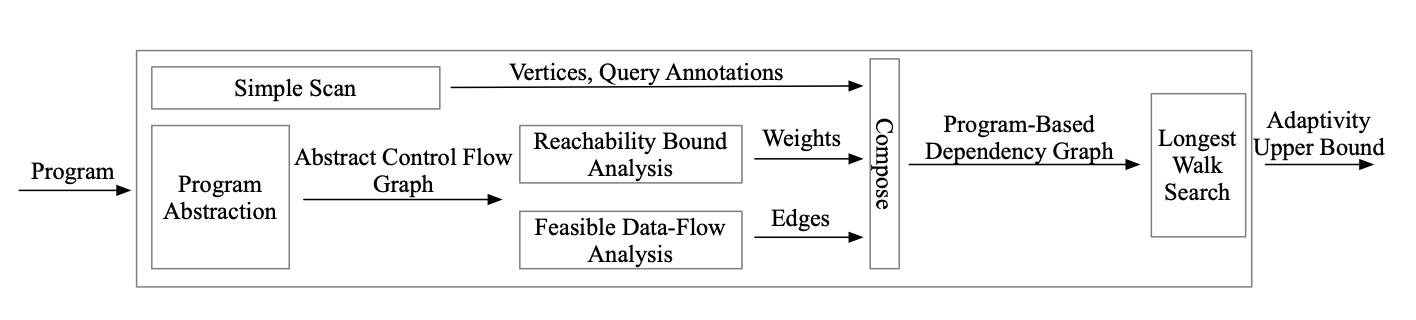
\includegraphics[width=1.0\columnwidth]{adapfun.png}
%   \vspace{-0.3cm}
%   \caption{The overview of {\THESYSTEM}}
%   \label{fig:adaptfun}
%   \vspace{-0.5cm}
% \end{figure}
%
%
\begin{enumerate}
\item  In Section~\ref{sec:abscfg}, we first construct an abstract control flow graph based on $c$, by computing an abstract transition 
for every labeled command. 
This graph is used in the following section from Section~\ref{sec:pathsensitive_rb-refine} to Section~\ref{sec:pathsensitive_rb-psrbcompute} for analyzing program's reachability bound.
% see Section~\ref{sec:alg_vertexgen}
\item Section~\ref{sec:pathsensitive_rb-refine} refines this program path sensitively, based on the abstract control flow graph.
\item Section~\ref{sec:pathsensitive_rb-lbcompute} estimates path-insensitive reachability upper bound for every while loop command in $c$.
\item Section~\ref{sec:pathsensitive_rb-outinalg} performs the Outside-In compute path-sensitive local bounds.
\item Section~\ref{sec:pathsensitive_rb-inoutalg} computes path-sensitive reachability bound for each edge on the abstract control flow graph.
\item Section~\ref{sec:pathsensitive_rb-psrbcompute} computes the path-sensitive reachability bound for every label in this program $c$ by summarizing 
the path-sensitive reachability bound of each edge on the abstract control flow graph.
% \item The Section~\ref{sec:reachabilitybound_algorithm} computes program's reachability bound in two steps as follows.
\end{enumerate}
% Finally, with all the ingredients ready, we construct the final approximated program-based dependency graph in Section~\ref{sec:alg_graphgen}

% the algorithm  without extra static analysis technique.
% \\
% Overall, this program-based graph has a similar topology structure as 
% % the one
% % of 
% the Execution-Based Dependency Graph. It has the same
% vertices and query annotations, but approximated edges and weights. We call the graph generated by static analysis techniques, static analysis dedendency graph. 
% \item Then in the last phase in Section~\ref{sec:alg_adaptcompute}, $\THESYSTEM$
% % we compute the upper bound for adaptivity over this approximated graph:
% % , as an upper bound for
% % program's adaptivity
% computes the upper bound for adaptivity over this approximated graph.
% in the last phase of this algorithm in Section~\ref{sec:alg_adaptcompute}.
% \subsection{Adaptivity Based on Program Analysis in \THESYSTEM}
% In order to give a bound on the program's adaptivity, we first build a
% program-based data-dependency graph to {over-}approximate the
% trace-based dependency graph.  Then, we define a program-based
% adaptivity over this approximated graph, as an upper bound for
% $A(c)$.
% %
% \subsection{ $\THESYSTEM$ Analysis Algorithm}
% \subsection{Dependency Graph Estimation}
% \subsection{Vertices Estimationn}
% \label{sec:alg_vertexgen}
% The first component of every vertex in the static analysis dependency graph are actually identical as the  Execution-Based Dependency Graph, which are assigned variables in the program annotated with the unique label(line number). 
% These vertices are collected by statically scanning the program, like what we do for vertices of its Execution-Based Dependency Graph. 
% The vertices are defined formally as follows.

%   \highlight{
% \[
%     \progV^0(c) \triangleq \left\{ 
%   (x^l, w) \in \mathcal{LV} \times \mathcal{A}_{\lin}
%   ~ \middle\vert ~
%   x^l \in \lvar(c)
%   \right\}
%   \]
%   }
%   %
% where $\mathcal{A}_{\lin}$ is the set of arithmetic expressions over $\mathbb{N}$ and program's input variables. 
% The weight $w$ for every vertex will be computed in following step in Section~\ref{sec:alg_weightgen}.
% The static scanning of the programs also tells us whether one vertice(assigned variable) is assigned by a query request. We have similar definition when defining the Execution-Based Dependency Graph, 
% a set of pairs $\progF(c) \in \mathcal{P}(\mathcal{LV} \times \{0, 1\} )$ 
% % is the set of pairs 
% % The weight for each vertex in $\progV(c)$ is computed 
% mapping each $x^l \in \progV(c)$ to a flag, either $0$ or $1$, where $1$  means $x^{l}$ is a member of $ \qvar_{c}$, a set of those variables assigned with query requests, and $0$ means $x^{l}$ not in this set. It is defined formally below.

% \[\progF(c) =\left\{(x^l, n)  \in  \mathcal{LV} \times \{0, 1\} 
% ~ \middle\vert ~
% x^l \in \lvar_{c},
% n = 1 \iff x^l \in \qvar_{c} \land n = 0 \iff  x^l \not\in \qvar_{c} .
% \right\}\]
%

% \wq{To do: Add $\THESYSTEM$, a data flow analysis algorithm to scan the program and give a graph.}
% {\THESYSTEM} consists of three phases: 
% \begin{enumerate}
%     \item Generating an abstract control flow graph with each edge representing an abstract event transiting between two command labels. 
%     \item Computing the value bound invariant for each variable in the event and 
%     the event transition closure over the abstract control flow graph,
%     we get the reachability bound for each labeled command.
%     \item Refining the abstract control flow graph with data-flow, by performing the reaching definition analysis, we generate a weighted data control flow graph.
%     \item An algorithm to find the appropriate path in the weighted data control flow graph
% \end{enumerate}

% \begin{enumerate}
%     \item An algorithm to generate a precise data control flow graph
%     \item An algorithm to perform a Reachability number analysis to calculate the weight of each node in the graph generated in phase 1.
%     \item An algorithm to find the appropriate path in the weighted data control flow graph
% \end{enumerate}

% \subsection{Edge and Weight Estimation}
% \label{sec:alg_weightedgegen}

% Since the edges of the execution-based graph of a program relies on the dependency relation, which handles both control flow and data flow, as an over-approximation of this graph, the edges of our static anlaysis dependency graph also covers these two kind of flows. We develop a feasible data flow relation to catch these two flows, in Section~\ref{sec:alg_edgegen}.


% The weight of every vertice in the execution-based graph is built on all possible execution traces.
% In order to over-approximate the weight statically but still tightly, we present a symbolic reachability bound analysis for estimation of the weight of each vertice(label) in Section~\ref{sec:alg_weightgen},
% in spirit of some reachablility bound techiniques.


% The edges and weight estimation are both performed on basis of an abstract control flow graph of the program, we first show how to generate this abstract execution control flow graph before the introduction of  the edge and weight estimation.  

% This analysis first 
%  generate an abstract control flow graph
%  over all program labels, 
% in order to analyzing the data flow relations through variables assigned in every labeled command,
% and the reaching time of each variable.
% Then, it refines this control flow graph 
% % into a weighted data-dependency graph, 
% and generate the Program-Based Dependency Graph,
% through the data flow and reaching bound analysis results.
% In the last step, it finds the longest finite walk in this weighted data control flow graph w.r.t. the query variables,
% and return the number of query vertices traversed alongside.
% % \wq{To do: Add $\THESYSTEM$, a data flow analysis algorithm to scan the program and give a graph.}
% To be more specific, {\THESYSTEM} consists of five phases as follows,
% \\
% % \jl{Better to have a graph or picture of overview of the algorithm}
% \todo{graph}
% \todo{pass again}
% This analysis
% \begin{enumerate}
%     % \item Generating 
%     \item first generate 
%     an abstract control flow graph
%     %  over all labels,
%     (remove?? with program's labels as vertices and abstract transitions as edges)
%     in Section~\ref{sec:abscfg},
%     % used to analyze 
%     for analyzing the weight of every vertex in $\progV(c)$ and edges between every vertex in $\progV(c)$ in the next two steps;
%     %  \ref{sec:alg_weightgen} and 
%     % \ref{sec:alg_edgegen}.

%     % which are used as program's control locations,
%     %
%     \item then use the abstract control flow graph generated above, 
%     compute the weight of every vertex in $\progV(c)$ by computing a symbolic reachability bound for each label in Section~\ref{sec:alg_weightgen},
%     % \\
%     \item and then use the same graph again to estimate the edges between every vertex in $\progV(c)$ by computing the feasible data flow relation between every labeled variables in Section~\ref{sec:alg_edgegen}.
  
% \end{enumerate}

\subsection{Abstract Execution Control Flow Graph}
\label{sec:abscfg}

This estimation is performed on basis of an abstract control flow graph of the program, 
we first show how to generate this abstract execution control flow graph before the introduction of  the edge and weight estimation.  
We discuss the vertices and edge of the
abstract control flow graph for a program $c$, $\absG(c)$.

\subsubsection{Vertices Construction}
\label{sec:abscfg-vertex}
Every 
vertex corresponds to the unique
label.
Specifically,
the vertices of this graph is the set of $c$'s labels with the exit label ${\lex}$, 
\[ 
  \absV(c) = \lvar(c)\cup\{{\lex}\}
  \]
%  corresponding to a label command in the program.

\subsubsection{Edge Construction}
\label{sec:abscfg-edge}
  Overall, the vertices can be easily collected and the key point of construction of the abstract execution
  control flow graph for a program is the abstract execution trace, 
  which relies on the abstraction of expression and abstract transition (we also call it abstract event).
  To make it easy to understand, abstract control flow graph is a control flow graph, with annotations on every edge.
It is generated as follows.
  % The edge in the abstract control flow graph comes from the abstract execution trace of the program. 
  % The abstract execution trace, an abstract representation of the execution, consists of a set of abstract events. 
%   The edge in the abstract control flow graph comes from the program's abstract events set $\absflow(c)$.
%   Each abstract event $(l_1, dc, l_2)$ in this set represents an edge in $\absE(c)$.
%   % Then, every abstract transition in the abstraction execution trace corresponds to an edge in the abstract control flow graph. In another word, the edge $(l_1, dc, l_2)$ in the abstract control flow graph, represents an abstract transition 
% %  from $l_1$ to $l_2$, with a set of difference constraints $dc$. 
%  Also notice, the difference constraints generated during the abstract transition appears in the edge as annotation.
%
\paragraph{Constraint Computation}
The constraint is computed for every expression in the program through expression abstraction.
\\
Operator: $\absexpr : \mathcal{A} \cup \mathcal{B} \to DC(\mathcal{VAR}  \cup \constdom) \cup \{\top\}$
\\
Constraints $\dcdom^{\top}: DC(\mathcal{VAR}  \cup \constdom) \cup \booldom \cup \top$ .
\\
Difference Constraints $DC(\mathcal{VAR}  \cup \constdom)$: 
\\
% The norms $\vnorm = \mathcal{VAR}  \cup \constdom $
The Symbolic Variables $\constdom = \mathbb{N} \cup \inpvar$, Boolean Expressions $\booldom$ and infinity $\top$.
\\
The set of all the inequality of form $x \leq y + v$ where $x \in \mathcal{VAR} $, 
$y \in \mathcal{VAR}$ and $v \in \constdom$.
\\
% $\cup$ Boolean Expressions $\booldom$ $\cup \top$ represents the infinity.
% The expression assigned to the variable on the left hand of the assignment command is abstracted to an abstract value: (adopted from the expression abstraction method in paper \cite{sinn2017complexity}). The abstract value is expressed in the form of Difference constraint, denotated as $DC : \mathcal{VAR} \cup \constdom \to \mathcal{\mathcal{VAR} \times (\mathcal{VAR} \cup \constdom) } \times (\mathbb{Z} \cup \{\infty\})$.  $\constdom$ is called the Symbolic Constant defined as $\constdom \triangleq \mathbb{N} \cup \inpvar$
% %  \cup \{\max{(\dbdom)}\} $, 
% which consists of 
% natural numbers $\mathbb{N}$,
% the program's input variables $\inpvar$. 
% % and a constant value $Q_m$ for estimating the upper bound of variables which are
% % assigned by queries. 

% Give an instance of difference constraint used here,
% $DC(\mathcal{VAR}  \cup \constdom) \cup \{\top\}$ represents all the difference constraints over 
% variable and symbolic constants. 
% % The difference constraint $DC$ over $\mathcal{VAR} \cup \constdom$ 
% It is a set of the inequality of form $x \leq y + v$ where $x \in \mathcal{VAR} $, 
% $y \in \mathcal{VAR}  \cup \constdom$ and $v \in \mathbb{Z}$. 
% This difference constraint is defined in the same way as
% \cite{sinn2017complexity}. For concise, we use $\dcdom^{\top}$ to represent the $DC(\mathcal{VAR}  \cup \constdom) \cup \{\top\} \cup \mathcal{BEXPR}$.

% We show the expression abstraction $\absexpr : \expr \to \mathcal{VAR} \to \dcdom^{\top} $ below.

% We introduce the following notations and operations first
% % an expression abstraction method based on the expression abstraction in paper \cite{sinn2017complexity}.
% \\
% % is enriched into $\constdom \triangleq \mathbb{N} \cup \inpvar \cup \{\max{(\dbdom)}\} $.
% T
% \\

% represents the set of inequality over all $\mathcal{VAR}  \cup \constdom$. 

% The symbolic constant is enriched into $\constdom \triangleq \mathbb{N} \cup \inpvar \cup \{\max{(\dbdom)}\} $.
% It consists of 
% natural number $\mathbb{N}$,
% the symbolic constants $\inpvar$ (i.e., the set of the program's input variables), 
% and a constant value $Q_m$ for estimating the upper bound of variables which are
% assigned by queries.
% \\
% The symbolic constant is enriched into $\constdom \triangleq \mathbb{N} \cup \inpvar \cup \{\max{(\dbdom)}\} $.
% \\

% % $ \absdom: \mathcal{P}(DC(\mathcal{VAR}  \cup \constdom) \cup \{\top \})$:
% \\
% $\constdom: \mathbb{N} \cup \inpvar \cup \{\max{(\dbdom)}\} $ 
% The  constant 
% \\
% % $DC(\mathcal{VAR}  \cup \constdom)$ represents the set of inequality over all $\mathcal{VAR}  \cup \constdom$.
% \\

% \[
%   \begin{array}{ll} 
%     \absexpr(y + c, x)  = x' \leq y + c  & c \in \mathbb{N} \land y \in (VAR \cup \constdom) \\
%     \absexpr(y - c, x)  = x' \leq y - c  & c \in \mathbb{N} \land y \in (VAR \cup \constdom) \\
%     \absexpr(v, x)  = x' \leq v + 0  & v \in (VAR \cup \constdom) \\
%     \absexpr(\aexpr, x) = x' \leq 0 + \infty   & \aexpr \text{ doesn't have any of the forms as above} \\
%     \absexpr(\qexpr, x)  = x' \leq 0 + Q_m & \qexpr \text{ is a query expression}  \\
%     \absexpr(\bexpr, x) = x' \leq 0 + 1   & \bexpr \text{ is a boolean expression} \\
%   \end{array}
%   \]
\begin{defn}{Expression Abstraction}
  \[
    \begin{array}{ll} 
      \absexpr(x - v, x)  = x' \leq x - v  & x \in \grdvar \land v \in \mathbb{N} \\
      \absexpr(y + v, x)  = x' \leq y + v  & x \in \grdvar \land v \in \mathbb{Z} \land y \in (\grdvar \cup \constdom) \\
      \absexpr(v, x)  = x' \leq v + 0  & x \in \grdvar \land v \in (\grdvar \cup \constdom) \\
      \absexpr(y + v, x)  = x' \leq y + v & \\
      \grdvar = \grdvar \cup \{y\} & x \in \grdvar \land v \in \mathbb{Z} \land y \notin (\grdvar \cup \constdom)  \\
      % \absexpr(\qexpr, x)  = x' \leq 0 + Q_m & x \in \grdvar \land \qexpr \text{ is a query expression}  \\
      \absexpr(\bexpr, \top) = \bexpr   & \\
      % \absexpr(y + v, x)  = x' \leq y + v & \\
      \grdvar = \grdvar \cup FV(\bexpr) &  x \in \grdvar \land \bexpr \text{ is a boolean expression} \\
      \absexpr(\expr, x) = x' \leq \infty  &  x \in \grdvar \land \expr \text{ doesn't have any of the forms as above} \\
      \absexpr(\expr, x) = \top  &  x \notin \grdvar \\
    \end{array}
    \]
  \end{defn}
  
  % \wq{ 
    $\grdvar$ is the set of variables used in the guard expression of every while command in the program $c$. 
  % }. 
  In the case 4, if a variable $x$, belonging to the set 
  $\grdvar$ is updated by a variable $y$, which isn't in this set, 
  we add $y$ into the set $\grdvar$ and repeat 
  above procedure  until $\grdvar$ and $\absexpr(\expr, x)$ is stabilized. 
  % \wq{I do not understand this sentence:-(}
  \\
Specifically 
% understanding the intuition, 
we handle a 
% simplified 
normalized guard expression ($ x > 0$ for $x^l \in \lvar_c$)
 in $\ewhile$, and 
%  \wq{I do not understand this sentence:-(}
%  .
% \\
% The counter variables only increase, decrease or reset by expression in the form of arithmetic minus and plus (able to extend to max and min.)
the counter variables only increase, decrease or reset by 
% expression in the form of 
simple arithmetic expression (mainly multiplication, division, minus and plus (able to extend to max and min)). 
This is the same as in paper \cite{sinn2017complexity}. 
\\
For more complex expression assignments, where the counter reset, or calculated from $\elog$, 
multiplication or division, and expressions involving multiple variables, the constraint is approximated as reset of $\infty$.
\\
% This simplification \wq{which part we simplify here?} 
This approximation strategy
doesn't affect our analysis results in our examples. It is easy to extend the normalized expression 
into more complex forms as in \cite{sinn2017complexity}, as well as the 
counter variable manipulation with more advanced expressions.
% \\ 
% The boolean expression in the guard of $\ewhile$ command is normalized into form of $ x > 0$ where $x^l \in \lvar_c$ for some $l$.
\begin{defn}[Symbolic Expression ($\mathcal{A}_{S}$)]
  $\mathcal{A}_{S}$ is the set of all the symbolic expressions 
over $\constdom$.
% For concise, $\mathcal{A}_{\lin}$ is used as the same meaning of $EXPR(\constdom)$ in the follows, to denote the arithmetic expression 
% over the symbolic variables, (i.e., $\mathbb{N}$ with input variables).
\end{defn}
The symbolic expression set is a subset of arithmetic expressions over $\mathbb{N}$ with input variables, 
i.e., $\mathcal{A}_{S} \subseteq \mathcal{A}_{\lin}$.
\subsubsection{Abstract Control Flow Graph through an Example}
\paragraph{Abstract Initial and Final State}
%
The abstract initial state: $\absinit(c) \in \ldom$,
The abstract Final State: $\absfinal(c) \in \mathcal{P}(\ldom \times \dcdom^{\top})$

The \emph{Abstract initial state} for a program $c$ is the initial label of this program.
This label corresponds to the first labeled command of this program 
when executing this program.
\\
Given a program $c$, its abstract initial state is computed as follows,
%
\[
  \begin{array}{ll}
    \absinit(\clabel{\assign{x}{\expr}}{}^l)  & = l  \\
    \absinit(\clabel{\assign{x}{\expr}}{}^l)  & = l \\
    \absinit(\clabel{\eskip}^{l})  & = l \\
    \absinit(\eif [b]^l \ethen c_1 \eelse c_2)  & = l \\
    \absinit(\ewhile [b]^l \edo c)  & = l \\
    \absinit(c_1 ; c_2)  & = \absinit(c_1) \\
 \end{array}
 \]
%

The \emph{Abstract Final State} of the program $c$, 
$\absfinal(c) \in \mathcal{P}(\ldom \times \dcdom^{\top})$
is a set of pairs, with a label as first component and a constraint as the second component.
Every pair in $\absfinal(c)$ corresponds to a labeled command of $c$,
and the constraint in this pair is computed by $\absexpr$ in the first step.
\\
Given a program $c$, its final state is computed as follows,
$\absfinal: \cdom \to \mathcal{P}(\ldom \times \dcdom^{\top})$,
% computes the set of Abstract Final State for the command. 
 \[
  \begin{array}{ll}
    \absfinal(\clabel{\assign{x}{\expr}}{}^l)  & = \{(l, \absexpr\eapp (\expr, x))\}  \\
    %  \absfinal(\clabel{\assign{x}{\query(\qexpr)}}{}^l)  & = \{
    %   (l, x' \leq 0 + Q_m )\}  \\
     \absfinal(\clabel{\eskip}^{l})  
     & = \{(l, \top)\} \\
     \absfinal(\eif [b]^l \ethen c_1 \eelse c_2)  & = \absfinal(c_1) \cup \absfinal(c_2) \\
     \absfinal(\ewhile [b]^l \edo c)  & = \{(l, \absexpr(\bexpr, \top))\} \\
     \absfinal(c_1 ; c_2)  & =  \absfinal(c_2) \\
 \end{array}
 \]
 %
 \paragraph{Abstract Event} 
 \emph{Abstract Event}: 
   $\absevent \in $
   $\ldom \times \dcdom^{\top} \times \ldom$
  % \emph{Abstract Execution Trace}: $\absflow \in \cdom \to \mathcal{P}( \ldom \times \dcdom^{\top} \times \ldom )$

 The abstract event is computed for w.r.t the program in Definition~\ref{def:absevent_compute}, 
%  generated during computing its abstract execution trace, 
its type is defined as follows,
 \begin{defn}[Abstract Event]
   \label{def:abs_event}
   Abstract Event: 
   $\absevent \in $
   $\ldom \times \dcdom^{\top} \times \ldom$
   is a 
   % pair of abstract initial state and final state.
   triple where the first and third components are labels,
   second component is a constraint from $\dcdom^{\top}$.
   % the thrid % computed from program's abstract final and initial state, $\absfinal(c)$ and $\absinit(c)$ with formal definition, and algorithm detail in Appendix.
   %  the constraint and the third corresponds to a final state.
   \end{defn}
   Specifically, in an abstract event, 
   the first label correspond to an initial state, and 
   the second label and the constraint correspond to an abstract final state.
  The abstract initial state is a label from $\ldom$.
 The abstract final state is a pair from $\ldom \times \dcdom^{\top}$,  
 where first component is a label from $\ldom$ and the second component is a constraint from $\dcdom^{\top}$.
 %
 For simplicity, we use $\mathcal{P}(\absevent)$ represent the power set of all abstract events.
%  , and we have $\absflow(c) \in \mathcal{P}(\absevent)$.

%  Now, we  extract the abstract execution trace  $\absflow(c)$ for a program, which computes the 
%  The \emph{Abstract Execution Trace} for program $c$ is a s
The set of the abstract events $\absflow(c)$ for a program $c$
% .
%  Its type is formally defined 
is computed as follows in Definition~\ref{def:absevent_compute}.
 %
 \begin{defn}[Computing Abstract Events]
 \label{def:absevent_compute}
  $\absflow \in \cdom \to \mathcal{P}( \ldom \times \dcdom^{\top} \times \ldom )$
  \end{defn}
 %
 The \emph{Abstract Execution Trace} for program $c$ is computed as follows.
 \\
  % We now show how to compute the abstract execution trace. 
 We first append a $\eskip$ command with 
%  a symbolic label $l_e$, i.e., $\clabel{\eskip}^{l_e}$ at the end of the program $c$, and compute the $\absflow(c) = \absflow'(c')$ for $c'$, where $c' = c;\clabel{\eskip}^{l_e}$ as follows,
the label $\lex$, i.e., $\clabel{\eskip}^{l_{ex}}$ at the end of the program $c$, and construct 
the program $c' = c;\clabel{\eskip}^{l_{ex}}$.
Then, we compute the $\absflow(c) = \absflow'(c')$ for $c'$ as follows,
 %
 {\footnotesize
 \[
   \begin{array}{ll}
      \absflow'(\clabel{\assign{x}{\expr}}{}^l)  & = \emptyset  \\
      \absflow'(\clabel{\assign{x}{\query(\qexpr)}}{}^l)  & = \emptyset  \\
      \absflow'([\eskip]^{l})  & = \emptyset \\
      \absflow'(\eif [b]^l \ethen c_t \eelse c_f)  & =  \absflow'(c_t) \cup \absflow'(c_f)
        \\ & \quad 
        \cup \{(l, \absexpr(\bexpr, \top),  \absinit(c_t) ) ,  (l, \absexpr(\neg\bexpr, \top), \absinit(c_f)) \} \\
       \absflow'(\ewhile [b]^l \edo c_w)  & =  \absflow'(c_w) \cup \{(l, \absexpr(\bexpr, \top), \absinit(c_w)) \} 
       \\ & \quad 
       \cup \{(l', dc, l)| (l', dc) \in \absfinal(c_w) \} \\
       \absflow'(c_1 ; c_2)  & = \absflow'(c_1) \cup  \absflow'(c_2) 
       \\ & \quad 
       \cup \{ (l, dc, \absinit(c_2)) | (l, dc) \in \absfinal(c_1) \} \\
   \end{array}
   \]
   }
   Notice $\absflow'([x := \expr]^{l})$, $\absflow'([x := \query(\qexpr)]^{l})$ and $\absflow'([\eskip]^{l})$ are all empty set. 
   For every event $\event$ with label $l$ in an execution trace $\trace$ of program $c$, 
   there is an abstract event in program's abstract execution trace of form $(l, \_, \_)$.  
   We also show the soundness of the abstract events computation in Appendix.
  %  which says 
  %  \wq{...}
   \begin{lem}[Soundness of the Abstract Events Computation]
     \label{lem:abscfg_sound}
   Given a program ${c}$, we have:
   %
   \[
     \begin{array}{l}
       \forall \vtrace_0, \trace \in \mathcal{T} ,  \event = (\_, l, \_) \in \eventset \st
   \config{{c}, \trace_0} \to^{*} \config{\eskip, \trace_0 \tracecat \vtrace} 
   \land \event \in \trace 
   \\
   \qquad \implies \exists \absevent = (l, \_, \_) \in (\ldom\times \dcdom^{\top} \times \ldom) \st 
   \absevent \in \absflow(c)
   \end{array}
   \]
   \end{lem}
%    This lemma is proved formally in Appendix~\ref{apdx:pathinsensitive_rb_soundness}.
% For every event $\event$ with label $l$ in an execution trace $\trace$ of program $c$, 
% there is an abstract event in program's abstract events computation of form $(l, \_, \_)$. 
This lemma is proved formally in Lemma~\ref{lem:abscfg_sound} in Appendix~\ref{apdx:pathinsensitive_rb_soundness}.
\\
For every labeled variable in program $c$, $x^l \in \lvar_c$, 
there is a unique abstract event in the program's abstract events set $\absevent \in \absflow(c)$ of form $(l, \_, \_)$. 
\begin{lem}[Uniqueness of the Abstract Events Computation]
  \label{lem:abscfg_unique}
Given a program ${c}$, we have:
%
\[
  \begin{array}{l}
    \forall \vtrace_0, \trace \in \mathcal{T} ,  \event = (\_, l, \_, \_) \in \eventset^{\asn} \st
\config{{c}, \trace_0} \to^{*} \config{\eskip, \trace_0 \tracecat \vtrace} 
\land \event \in \trace 
\\
\qquad \implies \exists! \absevent = (l, \_, \_) \in (\ldom\times \dcdom^{\top} \times \ldom) \st 
\absevent \in \absflow(c)
\end{array}
\]
\end{lem}
This lemma and proof is also 
formalized in Lemma~\ref{lem:absevent_unique} in Appendix~\ref{apdx:pathinsensitive_rb_soundness}.

  \paragraph{Edge Construction}
  we build the edge for $c$'s abstract control flow graph as follos,
  \[
    \absE(c) = \{(l_1, dc, l_2) | (l_1, dc, l_2) \in \absflow(c)\}
    \]
    The edge in the abstract control flow graph comes from the program's abstract events set $\absflow(c)$.
  Each abstract event $(l_1, dc, l_2)$ in this set represents an edge in $\absE(c)$.
  % Then, every abstract transition in the abstraction execution trace corresponds to an edge in the abstract control flow graph. In another word, the edge $(l_1, dc, l_2)$ in the abstract control flow graph, represents an abstract transition 
%  from $l_1$ to $l_2$, with a set of difference constraints $dc$. 
 Also notice, the difference constraints generated during the abstract transition appears in the edge as annotation.
% We have a pre-processing algorithm to go through the programs and returns the list of labels associating with a loop and whose visiting times need to be analyzed.
%
\subsubsection{Abstract Control Flow Graph} 
With the vertices $\absV(c)$ and edges $\absE(c)$ ready, we construct the abstract control flow graph, formally 
% Through a program $c$'s abstract events computation, its abstract control flow graph is computed 
defined in 
Definition~\ref{def:abs_cfg}.
%
\begin{defn}[Abstract Control Flow Graph]
\label{def:abs_cfg}
Given a program $c$, 
with its abstract control flow $\absflow(c)$
its abstract control flow graph $\absG(c) =(\absV(c), \absE(c), \absW(c))$ is defined as follows,
\\
$\absE(c) = \{(l_1, dc, l_2) | (l_1, dc, l_2) \in \absflow(c)\}$,
\\
$\absV(c) = \lvar(c)\cup\{l_{ex}\}$
% \\
%  $\absW(c) 
% \triangleq \left\{ (l, w) \in \mathbb{L} \times EXPR(\constdom) \right\}$.
\end{defn}
% \\
% Notice we also define the $\absW(c)$ in this graph without giving an actual value.
% This $\absW(c)$ is the set of weight for every 
% % vertex 
% label. 
% The weight $w \in EXPR(\constdom)$ is a symbolic expression over the symbolic constant, 
% which is the estimated upper bound on the number of visiting time for every control location
% through the reachability bound analysis as follows.
%
% $EXPR(\constdom)$ is the set of all the symbolic expressions 
% over $\constdom$, which is a subset of arithmetic expressions over $\mathbb{N}$ with input variables.
% For concise, $\mathcal{A}_{\lin}$ is used as the same meaning of $EXPR(\constdom)$ in the follows, to denote the arithmetic expression 
% over the symbolic variables, (i.e., $\mathbb{N}$ with input variables).
\subsubsection{Abstract Control Flow Graph through an Example}
\label{sec:abscfg_example}
% 
% Look at the two-round example again, its generated abstract control is shown as in Figure~\ref{fig:adapfun_tworound}(a).
% In this abstract control flow graph, every vertex is a label,
% corresponding to a label command in the program.
% Each directed 
% edge represents an abstract transition 
% between two control locations, 
% i.e., the labels of two commands (we call the labels also control location and they refer to the same thing), 
% where the second labeled command will be executed after execution of the command with first label.
% For example, the edge $0, a \leq 0, 1$ on the top, represents,
% from location $0$, the command 
% $\clabel{\assign{a}{0}}^0$ is executed with next continuation location $1$,
% where the 
% command $\clabel{\assign{j}{k}}^1$ will be executed next.
% The constraint $a \leq 0$ is generated by abstracting from the assignment command $\assign{a}{0}$,
% representing that value of $a$ is less than or equals to $0$ after 
% location $0$ before executing command at line $1$.
% %
% The same way for the rest edges' constructions.
%
\begin{example}[The Abstract Control Flow Graph for A Simple While Loop Program]
  \label{ex:whileSim_abscfg}
    For the simple while loop example program, 
its abstract control flow graph is shown as in Figure~\ref{fig:whileSim_abscfg}(b).
For example, the edge $(0, a' \leq 0, 1)$ on the top, tells us the command 
$\clabel{\assign{a}{0}}^0$ is executed with next continuation point $1$,
where the 
command $\clabel{\assign{j}{k}}^1$ will be executed next.
The constraint $a' \leq 0$ is a difference constraint, generated by abstracting from the assignment command $\assign{a}{0}$.
It represents that the value of $a$ is less than or equals to $0$ after 
execution of $\clabel{\assign{a}{0}}^0$ and before executing $\clabel{\assign{j}{k}}^1$.
The difference constraint is an inequality relation, 
the left-hand side of the inequality $x'$ denotes the variable $x$
after executing the command at $l$
and the right-hand side describes the variable $x$ in the state before the execution. 
Look at the $a' < a+x $ on the edge $5$ to $2$, which describes the execution of the command at line $5$, 
which is an assignment $a' = a+x$. The $a'$ on the left side of $a' < a+x$ represents the value of $a$ after the assignment,
while the right-hand side $a$ stores the value before the assignment. 
% $top$ means there is no assignment executed, for example, 
I have 
The boolean constraint $j \leq 0 $ on the edge $2 \to 6$, 
represents the negation of the testing guard $j > 0$
in the $\ewhile$ command with loop header at line $2$.
%
% The same way for the rest edges' constructions.
\begin{figure} 
  \centering
  \begin{subfigure}{.7\textwidth}
  \begin{centering}
  {\small
  $
  \kw{whileSim(k)} \triangleq
    \begin{array}{l}
        \clabel{ \assign{a}{0}}^{0} ;   
              \clabel{\assign{j}{k} }^{1} ;\\
              \ewhile ~ \clabel{j > 0}^{2} ~ \edo ~ 
              \Big(
               \clabel{\assign{x}{j} }^{3}  ;
               \clabel{\assign{j}{j-1}}^{4} ;
              \clabel{\assign{a}{x + a}}^{5}  \Big);\\
              \clabel{\assign{l}{k * a} }^{6}
          \end{array}
  $
  }
  \caption{}
  \end{centering}
  \end{subfigure}
    \begin{subfigure}{.45\textwidth}
    \begin{centering}
  \begin{tikzpicture}[scale=\textwidth/20cm,samples=200]
  \draw[] (-7, 10) circle (0pt) node{{ $0$}};
  \draw[] (0, 10) circle (0pt) node{{ $1$}};
  \draw[] (0, 7) circle (0pt) node{\textbf{$2$}};
  \draw[] (0, 4) circle (0pt) node{{ $3$}};
  \draw[] (0, 1) circle (0pt) node{{ $4$}};
  \draw[] (-7, 1) circle (0pt) node{{ $5$}};
  % Counter Variables
  \draw[] (6, 7) circle (0pt) node {\textbf{$6$}};
  \draw[] (6, 4) circle (0pt) node {{ $\lex$}};
  %
  % Control Flow Edges:
  \draw[ thick, -latex] (-6, 10)  -- node [above] {$a' \leq 0$}(-0.5, 10);
  \draw[ thick, -latex] (0, 9.5)  -- node [left] {$j' \leq k$} (0, 7.5) ;
  \draw[ thick, -latex] (0, 6.5)  -- node [right] {$j > 0$}  (0, 4.5);
  \draw[ thick, -latex] (0, 3.5)  -- node [right] {$x' \leq j$} (0, 1.5) ;
  \draw[ thick, -latex] (-0.5, 1)  -- node [above] {$j' \leq j - 1$} (-6, 1) ;
  \draw[ thick, -latex] (-6, 1.5)  -- node [left] {$a' \leq x + a$} (-0.5, 7)  ;
  \draw[ thick, -latex] (0.5, 7)  -- node [above] {$ j \leq 0 $}  (5.5, 7);
  \draw[ thick, -latex] (6, 6.5)  -- node [right] {$l' \leq k * a$} (6, 4.5) ;
  \end{tikzpicture}
  \caption{}
    \end{centering}
    \end{subfigure}
    \begin{subfigure}{.45\textwidth}
      \begin{centering}
    %   \todo{abstract-cfg for two round}
    \begin{tikzpicture}[scale=\textwidth/20cm,samples=200]
    \draw[] (-10, 10) circle (0pt) node{{ $0: 1$}};
    \draw[] (0, 10) circle (0pt) node{{ $1: 1$}};
    \draw[] (0, 7) circle (0pt) node{\textbf{$2: k$}};
    \draw[] (0, 4) circle (0pt) node{{ $3: k$}};
    \draw[] (0, 1) circle (0pt) node{{ $4: k$}};
    \draw[] (-10, 1) circle (0pt) node{{ $5: k$}};
    % Counter Variables
    \draw[] (6, 7) circle (0pt) node {\textbf{$6: 1$}};
    \draw[] (6, 4) circle (0pt) node {{ $\lex: 1$}};
    %
    % Control Flow Edges:
  \draw[ thick, -latex] (-8, 10)  -- node [above] {$a' \leq 0$}(-1.5, 10);
  \draw[ thick, -latex] (0, 9.5)  -- node [left] {$j' \leq k$} (0, 7.5) ;
  \draw[ thick, -latex] (0, 6.5)  -- node [right] {$j > 0 $}  (0, 4.5);
  \draw[ thick, -latex] (0, 3.5)  -- node [right] {$x' \leq j$} (0, 1.5) ;
  \draw[ thick, -latex] (-1.5, 1)  -- node [above] {$j' \leq j - 1$} (-8, 1) ;
  \draw[ thick, -latex] (-8, 1.5)  -- node [left] {$a' \leq x + a$} (-1.5, 7)  ;
  \draw[ thick, -latex] (1.5, 7)  -- node [above] {$j \leq 0 $}  (4.5, 7);
  \draw[ thick, -latex] (6, 6.5)  -- node [right] {$l' \leq k * a$} (6, 4.5) ;
    \end{tikzpicture}
    \caption{}
      \end{centering}
      \end{subfigure}
    \caption{(a) The Simple While Loop Example Program $\kw{whileSim(k)}$
    (b) The abstract control flow graph for $\kw{whileSim(k)}$  
    (c) The abstract control flow graph with the path insensitive reachability bound for $\kw{whileSim(k)}$.}
    \label{fig:whileSim_abscfg}
  \end{figure}
\end{example}
%
\subsection{\highlight{Program Refinement}}
\label{sec:pathsensitive_rb-refine}
In order to analyze the reachability bound path-sensitively, we first rewrite this program through two steps.

  \paragraph{Simple Transition Path Computation}
%
Every \emph{simple transition path},
either contains one simple loop starting from a loop header $l$ and go back to the same loop header $l$;
or doesn't constraint loop and starting from a loop header $l$ and go to a different loop header $l'$.
  \begin{defn}[Simple Tansition Path]
  A simple transition path
  $\tpath \in \paths(\absG(c))$, is a path on this program's abstract control flow graph $\absG(c)$ with 
  \\
  vertices sequence $(l_1 \to \cdots \to l_n)$ and
  \\
  edge sequence $(l_i, dc_i, l_{i + 1}) \in \absE(c)$ for every $i = 0, \cdots, n-1$,
  \\
  satisfying $l_i \neq l_j$ for all $l_i, l_j \in (l_1 \to \cdots \to l_{n - 1})$,
  and $l_1, l_n$ are both the control locations of loop headers.
  \end{defn}

  % For the part of the graph not in any SCC:

  % and end of $p'$ are both $l$;
  % \\
  %
% \item 
\paragraph{Repeat Pattern Computation}
A Repeat Pattern ($\rprog \in \mathcal{P}({\absG(c)})$) is either a simple path or sequence of repeat patterns. 
\[
  \rprog := \tpath | \rprepeat(\tpath) | \rprog; \rprog
\]
Every $\rprog$ can consecutively execute at least twice, and
 every sub-repeat patterns are distinct.
%  , i.e.,
% $rprog_i, rprog_j \in \rprog_1; \cdots; \rprog_n$, $\rprog_i \neq \rprog_j$.
% \\
\begin{defn}[Repeat Pattern]
  A simple path or sequence of repeat patterns
  $$
  \rprog := \tpath | \rprog; \rprepeat(\tpath) | \rprepeat(\tpath); \rprog
  $$ 
  satisfying,
  \\
  $\rprog$ can consecutively execute at least twice, and
  \\
  for every 
  $\rprog_i, \rprog_j \in \rprog_1; \cdots; \rprog_n$, $\rprog_i \neq \rprog_j$.
\end{defn}
%
Computation Steps:
\\
Through Path-Sensitive Refinement / Contexturalization algorithm \cite{GulwaniJK09, ZulegerGSV11},
this step computes the repeat patterns over all \emph{simple transition path}s.
\\
  Refined program:
  $\rprog \in \mathcal{RP}$.
  % For a Loop $L$,
  % computes all the transition Paths : $\tpath \in \absG(c)$
  % ->  $\rprog \in \mathcal{RP}$
  % in this loop and generate the refined statement.
  \\
  $p \triangleq \tpath $ if $\tpath \in \paths(\absG(c))$ and $\tpath \not\in SCC(\absG(c))$;
  \\
  $p \triangleq \rpchoose\{p_1, p_2 \}$ if $p_1$ and $p_2$ has the same head and end;
  \\
  $p \triangleq p_1; p_2$ if head of $p_1$ is the same as head of $p_2$ and either $p_1$ or $p_2$ isn't a simple path. 
  % \\
  % For the part of the graph not in some SCCs:
  % \\
  % For every while loop with guard label $l$:
  % \\
  % $p \triangleq \tpath $ if $\tpath \in \paths(\absG(c))$
  \\
  $p \triangleq L_l : \rprepeat(\rpchoose\{p_1, \cdots, p_m\})$ if head and end of $p'$ are both $l$;
  
  Given a rephrased program $p$, its refined program is computed as follows,
  \\
  $\rprog \triangleq \tpath $ if $p = \tpath$\\
  $\rprog \triangleq \rpchoose\{\rprog_1, \rprog_2 \}$ where $p \triangleq \rpchoose\{p_1, p_2 \}$ and 
    $\rprog_1$ and $\rprog_2$ are refined $p_1$ and $p_2$. 
    \\
  $\rprog \triangleq L_l : \kw{REFINE(p_w)}$  if $p = \rprepeat(p_w)$ and  $\kw{REFINE(p_w)}$ is the algorithm in \\
  $\rprog \triangleq \kw{REFINE(p_1)}; \kw{REFINE(p_2)}$  if $p = p_1; p_2$ 
\paragraph{Step3: Generate the Refined Program}.
\\
For every loop $L$ with the header at location $l$,
recursively 
find all the repeat patterns $\rprog_l$ starting form $l$ and go back to $l$.
\\
Adding a loop head annotation $L$ on the beginning of every repeat pattern $L: \rprog_l$.
\\
Generating the repeat pattern set $\rpchoose(l) \in \mathcal{P}(\paths(\absG(c)))$
for every loop $L$ with the header at location $l$,
$$\rpchoose(l) \triangleq \{ \rprog_l \}.$$
% \\%
Generating the Refined Program,
%
$$\rprog \triangleq \tpath_0; \rpchoose(l) ; \tpath_1; \cdots; \tpath_{\lex}.$$
%
$\tpath_i$ is the simple path that is not in any while loop,
and $\tpath_{\lex}$ is the simple path going to the program exit point.
% \end{enumerate}
%
% In order to estimate weight for every vertex in $\progV(c)$,
%  we first show how to compute the reachability bound for every label in $c$
%  % (i.e., every vertex in $\absV(c)$)
%  (i.e., the $\absW(c)$), 
%  then show how to compute the weight for every vertex in $\progV(c)$.
%  \\
%  Through the edges in $\absG(c)$, which correspond to $c$'s abstract transition between labels,
%  \wq{In order to estimate weight for every vertex in the static analysis dependency graph($\progV(c)$), we want to find out the upper bound on 
%  the number of times the labeled command (uniquely associated with a vertex in $\progV(c)$) may be executed when running the program.
%  This information can be obtained by computing the reachability bound for every vertice in the abstract control flow graph ($\absW(c)$), because
%  the vertices in the two graph share the same unique label, the line number. We can easily show that the reachability bound on one vertex of the actract control flow graph is also the upper bound for the corresponding vertex in the static analysis dependency graph, both vertices share the same unique line number.}
%  We perform the symbolic reachability bound anaysis on the abstract control flow graph, 
%  through the edges in $\absG(c)$, which correspond to $c$'s abstract transition between labels.
%  we infer the invariant for every variable, and compute the transition closure for every abstract transition. By solving the closure
%  with the invariants of variables involved in this closure for every transition, we compute
%  the symbolic reachability bound of every commands corresponding to this transition.
%  \\
%  Specifically in four steps, Variable Modification Tracking, Local Bounds Computation,
%  the symbolic reachability bound of every commands corresponding to this transition. Specifically, this analysis can be performed in four steps:
%   Variable Modification Tracking, Local Bounds Computation,
%  Invariant Inference and Closure Generation, and Reachability Bound Computation,
% {In order to estimate weight for every vertex in the static analysis dependency graph($\progV(c)$), we want to find out the upper bound on 
% the number of times the labeled command (uniquely associated with a vertex in $\progV(c)$) may be executed when running the program.
% This information can be obtained by computing the reachability bound for every vertex in the abstract control flow graph ($\absW(c)$), because
% the vertices in the two graph share the same unique label, the line number. We can easily show that the reachability bound on one vertex of the abstract control flow graph is also the upper bound for the corresponding vertex in the static analysis dependency graph, both vertices share the same unique line number.}
% In order to compute the \emph{Path-Sensitive Reachability Bound}, this analysis firstly compute the \emph{Path-Insensitive Reachability Bound} for every transition.
% \\
\subsection{\highlight{Ranking Function / Local Bound Computation}}
\label{sec:pathsensitive_rb-lbcompute}
% The \emph{Path-Insensitive Reachability Bound} analysis is performed 
Ranking Function / Local Bound is computed on the abstract control flow graph, 
through the edges in $\absG(c)$.
Every edge in $\absG(c)$ corresponds to the program $c$'s abstract transition between a pair of two labels.
We infer the invariant for every variable, and compute the transition closure for every abstract transition. By solving the closure
with the invariants of variables involved in this closure for every transition, we compute
the symbolic reachability bound of every commands corresponding to this transition. Specifically, this analysis can be performed in four steps:
 Variable Modification Tracking, Local Bounds Computation,
Variable Invariant Computation and Closure Generation, and Reachability Bound Computation,
% 
% We present the details of invariant, closure generation, and reachability bound computation as follows.
with details as follows.
%
%
\paragraph*{Variable Modifications Collection}
Identify the abstract events where each variable is increased, decreased and reset:
\\
$\inc: \mathcal{VAR} \to \mathcal{P}(\absevent) $
the set of the abstract events where the variable increase.
\\
$\inc(x) = \{(\absevent, c) | \absevent = (l, l', x' \leq x + v)\}$
\\
$\reset: \mathcal{VAR} \to \mathcal{P}(\absevent) $
The set of the abstract events where the variable is reset.
\\
$\dec: \mathcal{VAR} \to \mathcal{P}(\absevent) $
The set of abstract events where the variable decrease.
% \\
% $\dec(x) = \{(\absevent, c) | \absevent = (l, l', x' \leq x - v)\}$
\\
$Incr(v) \triangleq \sum\limits_{(\absevent, c) \in \inc(v)}\{\absclr(\absevent) \times v\}$
%
Based on this, 
Instead of just identifying the abstract events where each variable is reset,
this improvement identifies the chain of the events where a given variable is reset by the 
variables of the abstract events through the chain.
\\
$\resetchain: \mathcal{VAR} \to \mathcal{P}(\mathcal{P}(\absevent)) $
The set of the chain of abstract events where the variable is reset through the chain.
%
\paragraph*{Assign Ranks / Local Bound to Edges}
\begin{defn}[Ranks / Local Bounds Generatation]
  \label{def:lbgen}
Given a program $c$ with its abstract control flow graph 
$\absG(c) = (\absV, \absE)$
\\
Local Bounds Computation:
$\locbound: \absevent \to \mathcal{VAR} \cup \constdom$.
%
\[ 
\begin{array}{ll}
  \locbound(\absevent) \triangleq 1 
  & \absevent \notin SCC(\absG(c))
  \\
  \locbound(\absevent) \triangleq (x, v) 
  & \absevent \in SCC(\absG(c)) \land \absevent \in \dec(x) \land  \absevent = (\_, \_ , x' \leq x - v) \\
  \locbound(\absevent) \triangleq (x, \max(\dec(x))) 
  & \absevent \in SCC(\absG(c)) \land 
  \absevent  \notin \bigcup_{x \in \mathcal{VAR}} \dec(x)
  \land \absevent \notin SCC(\absG(c) \setminus \dec(x)) 
\end{array}
  \]
\end{defn}
  The first case is straightforward. 
  For the label $l$ which is not in any while loop, 
  the labeled command with the label $l$ will be 
  evaluated at most once. 
  % we do not need to analyze the visiting times of every node in the graph from phase 1.
  The second and third cases are guaranteed by the \emph{Discussion on Soundness} in Section 4 in~\cite{sinn2017complexity}.
  Then soundness proof is in Lemma~\ref{lem:local_bound_sound} in Appendix~\ref{apdx:pathinsensitive_rb_soundness}.
%
% \paragraph*{Invariant Inference and Closure Generation }
% Then, computing the bound invariants for variables and the transition closures for abstract events:
% \\ 
% $ \varinvar: \mathcal{VAR} \cup \constdom \to EXPR(\constdom)$
% \\
% $\absclr: \absevent \to EXPR(\constdom)$
% \\
% $EXPR(\constdom)$ is symbolic expression 
% over $\constdom$, which is a subset of arithmetic expressions over $\mathbb{N}$ with input variables and $ $.
% We use $\mathcal{A}_{\lin}$ denotes the arithmetic expression 
% over the symbolic variables, (i.e., $\mathbb{N}$ with input variables and $ $).
% Then, the symbolic invariant for each variable 
% as well as the symbolic transition closure for each transition is calculated as follows:
% \[ 
% \begin{array}{lll}
%   \varinvar(x) & \triangleq c & c \in \constdom \\
%   \varinvar(x) & \triangleq Incr(v) + \max(\{\varinvar(a) + c | (t, a, c) \in \reset(x)\}) & c \notin \constdom
% \end{array}
% \]
% %
% \begin{defn}
%   \label{def:transition_closure_base}
% \[ 
% \begin{array}{lll}
%   \absclr(\absevent) 
%   & \triangleq x / v & \\ 
%   & \locbound(\absevent) = (x, v) \in \constdom \times \mathbb{N} & \\
%   \absclr(\absevent) 
%   & \triangleq (Incr(x) + 
%   \sum\limits_{(\absevent', y, v') \in \reset(x)}
%   \absclr(\absevent') \times \max(\varinvar(y) + v', 0) ) / v & \\
%   & \locbound(\absevent) = (x, v) \land x \notin \constdom & 
% \end{array}
%   \]
% \end{defn}
% %
% \paragraph*{Improved Variable Modification Tracking}
% \\
% $Incr(v) \triangleq \sum\limits_{(\absevent, c) \in \inc(v)}\{\absclr(\absevent) \times v\}$
%
\paragraph*{Ranks / Local Bounds Estimation}
% Then, computing the bound for vriables and the transition closures for abstract events:
First estimating the bounds on the (ranks'/ local bounds') maximum value.
% , the 
\\ 
$ \varinvar: \mathcal{VAR} \cup \constdom \to \mathcal{A}_{\lin}$
\\
$\absclr: \absevent \to \mathcal{A}_{\lin}$
\\
Then, the symbolic invariant for each variable 
as well as the symbolic transition closure for each transition is calculated as follows:
\[ 
\begin{array}{lll}
  \varinvar(x) & \triangleq c & c \in \constdom \\
  \varinvar(x) & \triangleq Incr(v) + \max(\{\varinvar(a) + c | (t, a, c) \in \reset(x)\}) & c \notin \constdom
\end{array}
\]
%
% \paragraph*{Path-Insensitive Loop Bound Computation}
Based on the bounds on ranks / local bounds' maximum value,
we estimate the bounds on the iteration times
% of the ranks / local bounds 
for each edge in a path-insensitive fashion.
% \\
% computing the loop bound in a path-insensitive way as the base step.
\\ 
$ \varinvar: \mathcal{VAR} \cup \constdom \to \mathcal{A}_{\lin}$
\\
$\absclr: \absevent \to \mathcal{A}_{\lin}$
\\
% Then, the symbolic invariant for each variable 
% as well as the symbolic transition closure for each transition is calculated as follows:
% \[ 
% \begin{array}{lll}
%   \varinvar(x) & \triangleq c & c \in \constdom \\
%   \varinvar(x) & \triangleq Incr(v) + \max(\{\varinvar(a) + c | (t, a, c) \in \reset(x)\}) & c \notin \constdom
% \end{array}
% \]
%
\begin{defn}
  \label{def:transition_closure}
\[ 
\begin{array}{lll}
  \absclr(\absevent) 
  & \triangleq x / v & \\ 
  & \locbound(\absevent) = (x, v) \in \constdom \times \mathbb{N} & \\
  \absclr(\absevent) 
  & \triangleq \Big(
    \sum\limits_{y \in \{ y ~|~ 
    ch \in \resetchain(x), (l_1, x, y, v, l_2) \in ch \} } Incr(x) & \\
    & \quad + 
  \sum\limits_{ch \in \resetchain(x)}
  \big( \min\limits_{\absevent' \in ch}({\absclr(\absevent')}) \times 
  \max(\varinvar(y) + \sum\limits_{(l_1, x, y, v, l_2) \in ch } v, 0)\big) \Big) / v & \\
  & \locbound(\absevent) = (x, v) \land x \notin \constdom & 
\end{array}
  \]
\end{defn}
  %
% \paragraph*{Adding the Reachability Bounds for Every Vertex in the Data-Control Flow Graph}
% Updating the weight of every vertex in the $\progG(c) = (\progV, \progE)$ for program $c$ generated from phase 1. 
% For every $x^l \in \progV$, find the abstract event $\absevent \in \absflow(c)$ of the form $(l, \_, \_)$, updating the $\progW(x^l) $ by the transition closure of this event.
% \\
% The \emph{Path-Insensitive Reachability Bound} 
\paragraph{Theorem Guarantee}
For a program $c$ is sound upper bound for every label $l$ in this program formally in Theorem~\ref{thm:pathinsensitive_rb_soundness}. 
Proof of this theorem is in Appendix~\ref{apdx:pathinsensitive_rb_soundness}.
%
\begin{thm}[Soundness of the Path-Insensitive Local Bound /Rank Estimation]
  \label{thm:pathinsensitive_rb_soundness}
Given a program ${c}$, for every label $l \in \lvar(c)$,
its \emph{Path-Insensitive Rank Bound} $w^p$ 
 is a sound upper bound for its 
 execution-based reachability bound $w^t$ 
 where $(l, w^p) \in \absW(c)$ and  $(l, w^t) \in \exeRB(c)$.
% $\traceG = (\traceV, \traceE, \traceW, \traceF)$, 
% we have:
  %
  \[
    \begin{array}{l}
      \forall c \in \cdom, l \in \lvar(c),\trace_0 \in \mathcal{T}_0(c), 
      \trace' \in \mathcal{T}, v \in \mathbb{N}
      % , (v, n) \in \mathcal{VAR} \times \mathbb{N} \times \mathbb{N}
       \st 
      %  \\ \quad
      (l, w_p) \in \absW(c)
      \land 
      (l, w_t) \in \exeRB(c)
      \\ \quad
      \land \config{{c}, \trace_0} \to^{*} \config{\eskip, \trace_0\tracecat\vtrace'} 
      \land 
      \config{w_{p}, \trace_0} \earrow v
      \implies
      % \right\} 
      w_{t}(\trace) \leq v
    \end{array}
    \]
\end{thm}

\subsection{Outside-In Algorithm}
\label{sec:pathsensitive_rb-outinalg}
%
% \\
For the refined program $\rprog \in \mathcal{RP}$, the \emph{Outside-In Algorithm}
computes the path-sensitive local bound 
% for the refined program $\rprog$ recursively 
$\outinB: \rprog \to \mathcal{A}_{in}$ as follows,
% \\
\\
The \emph{State}: 
$\absstate \in \mathcal{P}(\dcdom^{\top})$ : conjunctions of the edge annotations.
%  constraints.
\\
For a refined program ($\rprog$), there are the 
\\
\emph{Initial State} ($\rfinit(\rprog)$), 
\emph{Final State} ($\rffinal(\rprog)$), and \emph{Next State} ($\rfnext(\rprog)$)  $\in \absstate$.
% The \emph{Initial State}: $\rfinit : \rprog \to \absstate $.
\\
The \emph{Variable Grade Decedent}: $\varGD : \rprog \to \mathcal{A}_{in}$, is the set of the variables' variation in one iteration;
\\
Given a refined program $\rprog$, its path-sensitive local reachability bound is computed as follows,
\\
$\outinB(\rpchoose\{\rprog_i\}) =  \max\{\outinB(\rprog_i)\}$
\\
$\outinB(\rprepeat\{\rprog\}) =  \frac{\rfinit(\rprog) - \rffinal(\rprog)}{\varGD(\rprog)}$
\\
$\outinB(\rpseq(\rprog_1, \rprog_2)) =  \outinB(\rprog_1)+ \outinB( \rprog_2)$
\\
$\outinB(\tpath) =  1$.
\\
$\outinB(\rprepeat\{\rprog\})$ can also be computed using the algorithm
\\
$\kw{BOUNDFINDERD(INITD(c, l_0, \absinit(\rprog)), NEXTD(c, l_0, \absinit(\rprog), V_{\lin} )}$ 
in paper~\cite{GulwaniJK09} with equivalent results.
\\
% Formally defined as follows,
% \begin{defn}[Path-Sensitive Local Reachability Bound]
%   \label{def:pathsensitive_lrb}
% \end{defn}
The computations of the operations: $\rfinit(\rprog)$,
$\rffinal(\rprog)$ $\rfnext(\tpath)$ and $\varGD : \rprog \to \mathcal{A}_{in}$
are formally defined as follows,
\begin{itemize}
\item \emph{Initial State} ($\rfinit(\rprog)$).
\\
 For a refined program $\rprog$, its initial refined abstract $\rfinit(\rprog) \in \mathcal{P}(\absstate)$ is computed as follows,
\[
  \rfinit(\rprog) \triangleq 
  \bigwedge_{x \in VAR(\rprog)}
  \left\{ 
  x = v ~\middle\vert~ 
  v = arg\max_{l_1}\left\{ 
    v~\middle\vert~ 
    (v, \absevent) \in \reset(x) 
    \land \absevent = (l_1, dc, l_2)
    \land l_1 \leq \absinit(\rprog)
    \right\}
  \right\}
  \]
% \\
The $\rfinit : \rprog \to \absstate $  can also be computed using $INIT(c, l_0, \absinit(\rprog))$ algorithm in \cite{GulwaniJK09}. 
$INIT(c, l_0, \absinit(\rprog))$ computes the equivalent results.
%
\item  \emph{Final State} $\rffinal(\rprog) \in \absstate$.\\
The program $\rprog$'s final refined abstract state $\rffinal(\rprog) \in \mathcal{P}(\absstate) $ is computed as follows, 
\[
  \rffinal(\rprog) \triangleq 
  \bigwedge_{x \in VAR(\rprog)}
  \left\{ 
    \varinvar(x)
  \right\} \land \neg Invariant(\rprog)
  \]
  % \\
\item \emph{Next State} $\rfnext(\rprog) \in \absstate$.
\\
 For a transition path $\tpath \in \paths(\absG(c))$, its $\rfnext(\tpath)$ is computed as follows,
%
\[
  \begin{array}{l}
  \rfnext(\tpath) \triangleq 
  \bigwedge\limits_{x \in VAR(\rprog)}
  \left\{ 
    \begin{array}{l}
  x =   \sum\limits_{(x, \absevent) \in \inc(x) }\left\{ 
    \varinvar(y) + c ~\middle\vert~ \absevent = (l, (y, c), \_) \land l \in \lvar(\rprog)\right\}
    \\ \qquad 
    - \sum\limits_{(x, \absevent) \in dec(x) }\left\{ 
      \varinvar(y) + c ~\middle\vert~ \absevent = (l, (y, c), \_) \land l \in \lvar(\rprog) \right\}
    \end{array}
  \right\}
  \end{array}
\]
\item  The program $\rprog$'s Variable Gradient Decent set is computed as follows,
\\
$\varGD(\rpchoose\{\rprog_i\}) =  \max\{\varGD(\rprog_i)\}$
\\
$\varGD(\rprepeat\{\rprog\}) =  \outinB(\rprepeat\{\rprog\}) \times {\varGD(\rprog)}$
\\
$\varGD(\rpseq(\rprog_1, \rprog_2)) =  \varGD(\rprog_1)+ \varGD( \rprog_2)$
\\
$\varGD(\tpath) =  \rfinit(\tpath) - \rfnext(\tpath)$
\\
\end{itemize}
%
\subsection{Inside-Out Algorithm}
\label{sec:pathsensitive_rb-inoutalg}
For the refined program $\rprog \in \mathcal{RP}$, the \emph{Inside-Out Algorithm}
computes the path-sensitive bound on the iteration numbers for every simple transition path in this program $\rprog$,
through following steps.

\begin{enumerate}
  \item \emph{Local Repeat Chain Bound}.
  \\
  For every transition path $\tpath$, its \emph{Local Repeat Chain Bound} is the 
  path sensitive local bound for it, inside its closet while loop.
  It is computed as follows,
  \begin{enumerate}
\item \emph{Repeat Chain Set}
\\
\emph{Repeat Chain} $\rpch(L, \tpath) \in \mathcal{P}(\rprog)$.
\\
$L, \tpath$ 
repeat chain w.r.t a transition path
is a list of repeat pattern $\rprog$ with loop header annotation $L$,
and the $\tpath$ is contained by these repeat patterns recursively.
% inside the same while loop $L$ as the $\tpath$. It is computed as follows,
% For a refined while loop program $\rprog_{l} = L_l : \rprog \in \mathcal{RP}$, 
% with its refined statement $\rprog \in \mathcal{RP}$,
\\
\emph{Repeat chain set}
$\rpchset(L, \tpath, \rprog) \in \mathcal{P}(\mathcal{P}(\rprog))$.
\\
For each transition path in the refined program $\tpath \in \rprog$, 
its repeat chain set 
$\rpchset(L, \tpath, \rprog) \in \mathcal{P}(\mathcal{P}(\rprog))$
 is a set of all the repeat chains for $L, \tpath \in \rprog$ in this program.
 %
 \begin{defn}[Repeat China ($\rpch(L, \tpath) \in \mathcal{P}(\rprog)$)]
  \label{def:repeatchain}
 Every repeat chain is a list of refined program contained inside the same while loop $L$ as the $\tpath$. It is computed as follows,
\\
  % $\rpch(L_l, \tpath) \in \mathcal{P}(\rprog)$\\
  $\rpch(L, \tpath) \triangleq \rprog_n \to \rprog_{n-1} \to \cdots \to \tpath $
 such that 
 $\rprog_{i}= L : \rprepeat(\cdots, \rprog_{i - 1}, \cdots)$ and
 there isn't any loop label (i.e., $L'$) or $\rprepeat_i$ between $\rprog_{i}$ and $\rprog_{i - 1}$ for $i = n, \cdots, 1$.
\end{defn}
%
%
%
\begin{defn}[Repeat China Set ($\rpchset(L, \tpath, \rprog) \in \mathcal{P}(\mathcal{P}(\rprog))$)]
  \label{def:repeatchainset}
 Every repeat chain is a list of refined program contained inside the same while loop $L$ as the $\tpath$. It is computed as follows,
\\
 $\rpchset(L_l, \tpath, \rprog) \triangleq 
 \{\rpch(L, \tpath) ~|~  
 \forall \rprog' \in \rpch(L, \tpath) \st \rprog' \in \rprog \}$
%  \rprepeat(\rprog) \in \rpchoose() \rprepeat(\rprog) = \rpch(L_l, \tpath) \} \mathcal{P}(\rpch(L_l, \tpath))$
\end{defn}
 % \\
% 2. 
% collect the loop chain: 
% $lpchain : \tpath \to \mathcal{P}(\mathcal{P}(\rprog)))$
% \\
% $lpchain(\tpath) = \rprog_n \to \rprog_{n-1} \to \cdots \to \tpath$
% % such that there is at least a $\rpchoose$ and isn't consecutive repeats $\rprepeat$ (i.e., at most one 
% % $\rprepeat$) between any $\rprog_{i - 1}$ and $\rprog_{i}$ for $i = n, \cdots, 1$.
% $\rprog_{i}= \rprepeat^{L_i}(\cdots, \rprog_{i - 1}, \cdots)$ and
%  there isn't any loop (i.e., $\rprepeat^{L}$) between $\rprog_{i}$ and $\rprog_{i - 1}$ for $i = n, \cdots, 1$.
% \\
% 2. Compute the local bound for every repeat chain as follows:
% \\
% $\rpchB(L, \tpath) = \prod\limits_{\rprog_i \in rpchain(\tpath)}
% % \frac{chsInit(\rprog_i, \tpath) - chsFinal(\rprog_i, \tpath)}{\varGD(\rprog_i, \tpath)}
% \outinB(\rprog_i)$
% % \\
% where $\rprepeat^{L}$ is the closet loop containing $\tpath$, $\rprepeat^{L}(\cdots, \rprog, \cdots)$.
% \\
% 4. Compute the nested local bound for every loop chain as follows, for every of 
% $(\rprog_i, \tpath)$ such that $\rprog_i \in lpchain(\tpath)$,
% \\
% $\lpchB(\rprog_i, \tpath) = 
% % \prod\limits_{\rprog_i \in lpchain(\tpath)}
% \frac{\lpinit(\rprog_i, \tpath) - lpFinal(\rprog_i, \tpath)}{\varGD(\rprog_i, \tpath)}$
% \\
\item  \emph{Local Repeat Chain Bound}.
\\
For every transition path $\tpath$
in its closet enclosed while loop $L$,
the \emph{Local Repeat Chain Bound} $\rpchB(L, \tpath) \in \mathcal{A}_{in}$ is computed as follows,
% $rpRB: \tpath \to \mathcal{A}_{in}$, $chsRB: (\rprog \times \tpath) \to \mathcal{A}_{in}$
% \\
% For each transition path $\tpath \in \rprog$,
% \\
% 1. First compute the path sensitive reachability choosing bound through their choose chain:
% \\
% $chsRB(\rprog_n, \tpath) = \prod\limits_{\rprog_i \in lpchain(\rprog_n, \tpath)}
% \frac{chsInit(\rprog_i, \tpath) - chsFinal(\rprog_i, \tpath)}{\varGD(\rprog_i, \tpath)}$
  \\
  $\rpchB(L, \tpath) = \max \left\{ \prod\limits_{\rprog_i \in ch}  \outinB(\rprog_i) 
  ~\middle\vert~ ch \in \rpchset(L_l, \tpath) \right\}
  $;
  \\
  $\rpchB(L, \tpath) = \bot$ if $L$ isn't the closest while loop containing $\tpath$.
  %
  \end{enumerate}
% \\
% \\
% 2. Then compute the path sensitive reachability repeating bound for $\tpath$ as:
% \\
% $RB(\tpath) = \max\limits_{l \in lpchains(\tpath)} \{\rpchB(n, \tpath) \prod\limits_{\rprog_i \in l} lpRB(\rprog_i, \tpath) \}$
% % For $chain \in rpchain(\tpath)$:
% where $lpchains(\tpath)$ is set of $lpchains(\tpath)$ containing all the loop chains of $\tpath$.
%
\item \emph{Related Loop Bound}.
\\
For every transition path $\tpath \in \rprog$, 
the \emph{Nested Loop Bound} $\lpchB(L_i, \tpath, \rprog) \in \mathcal{A}_{\lin}$ is computed as follows.
\begin{enumerate}
  \item \emph{Nested Loop Chain}.
  Each loop chain $\lpch(\tpath, \rprog) \in \mathcal{P}(\rprog)$ 
  is a list of refined program $\rprog' \in \rprog$
  $\tpath$ is nested in, and every $\rprog'$ has different loop header annotation.
  \\
For each transition path in the refined program $\tpath \in \rprog$, 
its \emph{Loop Chain} is computed as follows,
% repeat chain.
% then there is loop tree as follows for a program:
% $P = \rprepeat^{L_n}(\cdots, \rprepeat^{L_{n'}}(\cdots), \cdots, \rprepeat^{L_{n''}}(\cdots))$.
% \\
% For each transition path $\tpath$, we:
% from the head of the while loop.
% 1. firstly collect the loop chain: 
% $lp\mathcal{C}(\tpath) \in \mathcal{P}(\mathcal{P}(\rprog)) \triangleq \mathcal{P}(\lpch(\tpath))$
\begin{defn}[Nested Loop Chain]
  \label{def:loopchain}
$\lpch(\tpath, \rprog) \in \mathcal{P}(\rprog) \triangleq 
L_n \to L_{n-1} \to \cdots \to \tpath$
\\
% such that there is at least a $\rpchoose$ and isn't consecutive repeats $\rprepeat$ (i.e., at most one 
% $\rprepeat$) between any $\rprog_{i - 1}$ and $\rprog_{i}$ for $i = n, \cdots, 1$.
such that 
$\rprog_{i}= L_i : (\cdots, L_{i - 1} : \rprog_{i-1}, \cdots)$ and
 there isn't any loop label (i.e., $L'$) between $\rprog_{i}$ and $\rprog_{i - 1}$ for $i = n, \cdots, 1$.
\end{defn}
\item  \emph{Related Loop Bound}.
$\lpchB(L_i, \tpath, \rprog) \in \mathcal{A}_{\lin}$.
\\
Given a loop label $L_i \in \rprog$ and a transition path $\tpath \in \rprog$ in a refined program $\rprog$,
the \emph{Related Loop Bound} $\lpchB(L_i, \tpath, \rprog)$ is a symbolic expression in $\mathcal{A}_{\lin}$.
\\
This expression is the path-sensitive
reachability bound on the number of $L_i$'s iteration numbers,
%  will 
% bound the execution times of $L_{t_0}$
% in each single execution of the $L_{t_i}$ for every
such that, during these iterations, $\tpath$ will be executed. 
%  bound of $\tpath$ in the while loop with loop label $L_i$.
\\
For a refined program $\rprog$, 
% with its refined statement $\rprog \in \mathcal{RP}$,
% \\
% for 
each transition path in this refined program, $\tpath \in \rprog$ with its loop chain set $\rpchset(\tpath)$,
\\
and every loop label $L_i \in \lpch(\tpath) $ and $\lpch(\tpath)  \in \rpchset(\tpath)$:
% \\
% $(L_i, \tpath)$ such that $L_i \in \lpch(\tpath)$,
\\
$\lpchB(L_i, \tpath, \rprog) = \rpchB(L_i, \tpath, \rprog)$ if $\rpchB(L_i, \tpath, \rprog) \neq \bot$.
\\
$\lpchB(L_i, \tpath, \rprog) = 
% \prod\limits_{\rprog_i \in lpchain(\tpath)}
\frac{\lpinit(L_i, \tpath) - \rffinal(\tpath)}{\lpinit(L_i, \tpath) - \lpnext(L_i, \tpath)}$
% \\
\begin{defn}[Related Loop Bound ($\lpchB(L_i, \tpath, \rprog) \in \mathcal{A}_{\lin}$)]
  \label{def:relatedloop_bound}
For each transition path in a refined program $\tpath \in \rprog$
and every loop $L_i \in \lpch(\tpath, \rprog)$,
% where $\lpch(\tpath)  \in \rpchset(\tpath)$, 
the \emph{Related Loop Bound} $\lpchB(L_i, \tpath, \rprog)$ is computed as follows,
\\
$\lpchB(L_i, \tpath, \rprog) = \rpchB(L_i, \tpath, \rprog)$ if $\rpchB(L_i, \tpath) \neq \bot$.
\\
$\lpchB(L_i, \tpath, \rprog) = 
% \prod\limits_{\rprog_i \in lpchain(\tpath)}
\frac{\lpinit(L_i, \tpath) - \rffinal(\tpath)}{\lpinit(L_i, \tpath) - \lpnext(L_i, \tpath)}$
\end{defn}
The computations of the operations $\lpinit(L_i, \tpath)$ and $\lpnext(L_i, \tpath)$
are formally computed as follows,
\begin{itemize}
\item For a transition path $\tpath \in \paths(\absG(c))$ and a loop label $L_i$ in this transition path's loop chain.
Let $\rprog_i$ be the refined program with this loop label $L_i$, i.e., $L_i: \rprog_i \in \rprog$, 
the abstract loop chain initial state $\lpinit(L_i, \tpath) \in \mathcal{P}(\absstate)$ is computed as follows,
\[
  \lpinit(L_i, \tpath) \triangleq 
  \bigwedge_{x \in VAR(c)}
  \left\{ 
  x = arg\max_{l_1}
  \left\{
      \begin{array}{l}
    (v, (l_1, dc, l_2)) \in \reset(x) 
        \\ 
    % \qquad
    \land \absinit(\rprog_i) \leq l_1 \leq \absinit(\tpath)
    \end{array}
    \right\}
  \right\}
  \]
\item
For a transition path $\tpath \in \paths(\absG(c))$ and a refined program $\rprog_i$ with the loop label $L_i: \rprog_i$, its $\rfnext(L_i, \tpath)$ is computed as follows,
%
\[
  \begin{array}{l}
  \lpnext(L_i, \tpath) \triangleq 
  \bigwedge\limits_{x \in VAR(\rprog)}
  \left\{ 
    \begin{array}{l}
  x =   \sum\limits_{(x, \absevent) \in \inc(x) }\left\{ 
    \varinvar(y) + c ~\middle\vert~ \absevent = (l, (y, c), \_) \land l \in \lvar(\rprog_i)\right\}
    \\ \qquad 
    - \sum\limits_{(x, \absevent) \in dec(x) }\left\{ 
      \varinvar(y) + c ~\middle\vert~ \absevent = (l, (y, c), \_) \land l \in \lvar(\rprog_i) \right\}
    \end{array}
  \right\}
  \end{array}
\]
$\lpinit(L_i, \tpath)$, and $\lpnext(L_i, \tpath)$ can be computed using the 
$INIT(c, i, \absinit(\tpath))$ and $NEXT(c, i, \absinit(\tpath))$ from paper \cite{GulwaniJK09}.
% \\
The $\lpchB(L_i, \tpath)$ can also be computed using the algorithm 
$\kw{BOUNDFINDERD(INIT(c, i, \absinit(\tpath)), NEXT(c, i, \absinit(\tpath)), V_{\ln})}$
from paper \cite{GulwaniJK09} with the equivalent result.
\end{itemize}
% $rpRB: \tpath \to \mathcal{A}_{in}$, $chsRB: (\rprog \times \tpath) \to \mathcal{A}_{in}$
% \\
% For each transition path $\tpath \in \rprog$,
% \\
% 1. First compute the path sensitive reachability choosing bound through their choose chain:
% \\
% $chsRB(\rprog_n, \tpath) = \prod\limits_{\rprog_i \in lpchain(\rprog_n, \tpath)}
% \frac{chsInit(\rprog_i, \tpath) - chsFinal(\rprog_i, \tpath)}{\varGD(\rprog_i, \tpath)}$
% \\
\end{enumerate}
\item The \emph{Inside-Out Bound} ($\inoutB(\tpath, \rprog) \in \mathcal{A}_{in}$).
\\
For every transition path $\tpath \in \rprog$, its \emph{Inside-Out Loop Bound}
 $\inoutB(\tpath, \rprog) \in \mathcal{A}_{in}$ is 
% Compute 
the path sensitive reachability bound on the iteration numbers of this path in this refined program $\rprog$. 
It is computed in Definition~\ref{def:outin_bound}.
\begin{defn}[{Inside-Out Loop Bound} ($\inoutB(\tpath, \rprog) \in \mathcal{A}_{in}$)]
  \label{def:outin_bound}
  Given a refined program $\rprog$, for every transition path $\tpath \in \rprog$, 
  its \emph{Inside-Out Loop Bound}
  $\inoutB(\tpath, \rprog)$ is 
 % Compute 
 computed as follows,
$\inoutB(\tpath, \rprog) =
  \prod\limits_{L \in \lpch(\tpath, \rprog)} \rpchB(L, \tpath, \rprog)
% lpRB(\rprog_i, \tpath) 
% ~ \middle\vert~ l \in lp\mathcal{C}(\tpath) \right
$
\end{defn}
% For $chain \in rpchain(\tpath)$:
% where $lpchains(\tpath)$ is set of $lpchains(\tpath)$ containing all the loop chains of $\tpath$.
\end{enumerate}
%
\subsection{Path Sensitive Reachability Bound Computation for Every Location}
\label{sec:pathsensitive_rb-psrbcompute}
$psRB(c, l) \in \mathcal{A}_{in}$
\\
For every program control location $l \in \lvar(c)$, with $\rprog$ as its refined program,
%  in a program $c$,
%  refined program $l \in \lvar(\rprog)$,
 $\psRB(l, \rprog)$ is its path sensitive reachability bound on the executing times of this location $l$.
 \\
 \begin{defn}
  \label{def:label_psrb}
Given a program $c$ with its refined program $\rprog \in \mathcal{RP}$
%  with 
% \emph{Global Loop Bound} $\inoutB(\tpath)$
% computed for its every transition path $\tpath \in \rprog$  notated by $\inoutB(\tpath)$,
%  for each of its transition path $\tpath \in \rprog$ 
% with the \emph{Global Loop Bound}
% computed as above, notated by $\inoutB(\tpath)$.
the $\psRB(c, l)$ for every label $l \in \lvar(c)$ is computed as follows,
\\
\[ \psRB(c, l) = \sum\limits_{\tpath \in \rprog \land 
l \in \tpath} \inoutB(\tpath)\]
 \end{defn}
\begin{thm}[Soundness of the Path Sensitive Reachability Bound Estimation]
  \label{thm:pathsensitive_rb_soundness}
Given a program ${c}$, for every label $l$ of this program $c$ such that $(l, w) \in \exeRB(c)$, 
and any initial trace $\trace_0 \in \mathcal{T}_0(c)$ with 
% $\config{{c}, \trace_0} \to^{*} \config{\eskip, \trace_0\tracecat \vtrace} $ 
and $\config{\psRB(c, l), \trace_0} \earrow v$,
% for some generated evaluation trace $\vtrace \in \mathcal{T}$,
we have $ w(\trace_0) \leq v $.
%
\[
  \begin{array}{l}
  \forall (l, w_{t}) \in \exeRB(c),
  % (x^l, w_{p}) \in \progV, 
  \trace_0 \in \mathcal{T}_0(c), 
  v \in \mathbb{N} \st
  \config{\psRB(c, l), \trace_0} \earrow v
  \implies
  % \right\} 
  w_{t}(\trace_0) \leq v
  \end{array}
\]
\end{thm}
%
Proof of this theorem is in Appendix~\ref{apdx:pathsensitive_rb_soundness}.
\paragraph*{Path Sensitive Reachability Bound through An Example}
\begin{example}
  [\todo{While Single Algorithm}]
  \label{ex:whileSigle}
  $$
  \kw{whileSim(k)} \triangleq
    \begin{array}{l}
        \clabel{ \assign{a}{0}}^{0} ;   
              \clabel{\assign{j}{k} }^{1} ;\\
              \ewhile ~ \clabel{j > 0}^{2} ~ \edo ~ 
              \Big(
               \clabel{\assign{x}{j} }^{3}  ;
               \clabel{\assign{j}{j-1}}^{4} ;
              \clabel{\assign{a}{x + a}}^{5}  \Big);\\
              \clabel{\assign{l}{k * a} }^{6}
          \end{array}
  $$
\end{example}
  % 
  \begin{enumerate}
    \item  \textbf{The Constraint Program (Abstract Control Flow Graph)}
    is illustrated in Example~\ref{ex:whileSim_abscfg} in Figure~\ref{fig:whileSim_abscfg}(b)
  
    \item \textbf{Program Refinement}
    \\
    The loop free simple transition paths are computed as follows,
    \\
  $\tpath_0 =  (0 \to 1), (1 \to 2)$
  \\
  $\tpath_1 =  (2 \to 3), (3 \to 4), (4 \to 5), (5 \to 2)$
  \\
  $\tpath_2 = (2 \to 6 \to \lex)$
  \\
  For simplicity, I omitted the vertices sequence and the constraints for every edge in the transition path. 
  In the following examples in Section~\ref{sec:example}, they 
  are omitted as well. 
  \\
  In this example the complete transition paths are as follows,
  \\
  $\tpath_0 =  
    \left\{ \begin{array}{l}
    \text{Edges Sequence}: ((0, a \leq 0, 1), (1, j \leq k, 2))
    \\
    \text{Vertices Sequence}: (0, 1, 2)
    \end{array}\right\}
  $
  \\
  $\tpath_1 =  
  \left\{ \begin{array}{l}
    \text{Edges Sequence}: ((2, j > 0, 3), (3, x \leq j, 4), (4, j \leq j - 1, 5), (5, a \leq x + a, 2))
    \\
    \text{Vertices Sequence}: (2, 3, 4, 5, 2)
    \end{array}\right\}
  $
  \\
  $\tpath_2 = 
  \left\{ \begin{array}{l}
    \text{Edges Sequence}: ((2, j \geq 0, 6), (6, l \leq k*a, \lex))
    \\
    \text{Vertices Sequence}: (2, 6, \lex)
    \end{array}\right\}
    $
  \\
  \textbf{Refined Program}:
  \[
    \tpath_0 ; 1: \rprepeat(\tpath_1); \tpath_2
  \]
  \item \textbf{Outside-In Algorithm}: The \emph{OutIn} bound for the $\rprog$ and every nested repeat patterns.
  \\
  $\outinB(\tpath_0) = 1$
  \quad
  $\outinB(\tpath_2) = 1$
  \quad
  $\outinB(\rprepeat_1(\tpath_1)) = k $
  % \\
  \item \textbf{Inside-Out Algorithm}
  \begin{itemize}
    \item \textbf{Repeat Chain Set}
    \\
    $\rpchset(1, \tpath_1) = \{\rprepeat_1(\tpath_1)\}$ 
    % \\
    % $\rpchset(1, \tpath_2) = \{\rprepeat_2(\tpath_2), \rprepeat_3(\rprepeat_2(\tpath_2); \tpath_1) \to \rprepeat_2(\tpath_2)\}$ \\
    $\rpchset(\_, \_) = \emptyset$ 
    % \\
    \item \textbf{Repeat Chain Bound} for every simple transition path $\tpath$ through its \emph{Repeat Chain}s
    \\
    $\rpchB(1, \tpath_1) = k$
    %
    \item \textbf{Loop Chain}
    \\
    $\lpch(\tpath_1) = 1\to \tpath_1$ \quad
    $\lpch(\tpath_0) = \tpath_0$ \quad
    $\lpch(\tpath_3) = \tpath_3$ 
    \item \textbf{{Relative Loop Bound}} for every simple transition path $\tpath$ through its \emph{Loop Chain}
    \\
    $\rpchB(1, \tpath_1) =   k$
  \quad
    $\rpchB(\bot, \tpath_0) = 1$ \quad
    $\rpchB(\bot, \tpath_2) = 1$ 
    \item \textbf{Path-Sensitive Reachability-Bound} for every simple transition path $\tpath$
    \\
    $\inoutB(\tpath_1) = k$
\quad
    $\inoutB(\tpath_0) = 1$ \\
    $\inoutB(\tpath_2) = 1$ 
  \end{itemize}
  \item Step 7: Path Sensitive Reachability Bound Computation for Every Location
  \\
  $\psRB(\{0, 1, 2\}) = 1$ \\
  $\psRB(\{3, 4, 5, 2 \}) = k$
   \\
  $\psRB(\{6, \lex\}) = 1$
  \end{enumerate}

% % % % 
\subsection{Constraint Program}
\label{sec:abs_prog}
% \textbf{Step 1: Program Abstract Execution Control Flow Graph}
The Constraint program is an Abstract Transition Graph,
% For a program $c$, this analysis first generates its abstract execution control flow graph notated as follows,
\[\absG(c) =(\absV(c), \absE(c)).\]
%
$\absV(c)$ is the set of program $c$'s control location, each edge in $\absE(c)$ is a transition
between two control locations if and only if there is a feasible control flow between the two locations.
Each edge is annotated by a difference constraint \cite{sinn2017complexity} or a boolean expression
from the set $\dcdom^{\top}$.
% (denoted by $\dcdom^{\top}$).
\\
\textbf{Components:} 
\\
The Vertices Set $\absV(c) = \lvar(c)\cup\{{\lex}\}$, is the set of program $c$'s control locations.
%  $\absV(c) = \lvar(c)\cup\{{\lex}\}$
\\
An edge $(l_1, dc, l_2) \in \ldom \times \dcdom^{\top} \times \ldom$, represents control flow from $l_1$ to $L_2$.
% such that control flow from $l_1$ to $l_2$.
\\
An annotation $ dc: \dcdom^{\top}$,
% Difference Constraints $\cup$ Boolean Expressions $\booldom$ $\cup \top$ represents the infinity.
describes the size change of the variables by executing commands from location $l_1$ to $l_2$.
\\
The annotation set $\dcdom^{\top}$: Difference Constraints $\cup$ Boolean Expressions $\booldom$ $\cup \top$ represents the infinity.
\\
\textbf{Generating Steps:} 
\\
Step1: generating control flow edges $(l_1, \_, l_2)$ for all the locations $l_1, l_2 \in \lvar(c)$.
\\
Step2: computing annotation $dc$ for each edge $(l_1, \_, l_2)$.
\\
Input the commands from location $l_1$ to $l_2$.
\\
Output: a set of $\dcdom^{\top}$.
\\
% Constraint Event: 1 edge of the Constraint Program, and 
% \\
% Constraint Execution Trace : the edge set of the Constraint Program.
\textbf{Theorem Guarantee:}
Soundness and Uniqueness.
\subsection{Constraint Program Refinement}
\label{sec:refine}
Algorithm Steps:
\\
\textbf{step1: Simple Transition Path Computation}.
\\
% Computes the Simple Transition Paths from Constraint Program,  
% 
Simple Transition Path: $\tpath \in \paths(\absG(c))$.
\\
For a constraint program $\absG(c)$,
every \emph{simple transition path} $\tpath \in \paths(\absG(c))$,
either contains one simple loop starting from a loop header $l$ and go back to the same loop header $l$;
or doesn't constraint loop and starting from a loop header $l$ and go to a different loop header $l'$.
\\
\textbf{Step2: Repeat Pattern Computation}.
\\
% Repeat Pattern $\rprog \in \mathcal{P}({\absG(c)})$.
% % \\
A Repeat Pattern ($\rprog \in \mathcal{P}({\absG(c)})$) is either a simple path or sequence of repeat patterns. 
\[
  \rprog := \tpath | \rprepeat(\tpath) | \rprog; \rprog
\]
Every $\rprog$ can consecutively execute at least twice, and
 every sub-repeat patterns are distinct, i.e.,
 $\rprog_i, \rprog_j \in \rprog_1; \cdots; \rprog_n$, $\rprog_i \neq \rprog_j$.
 \\
Through Path-Sensitive Refinement / Contextualization algorithm in \cite{GulwaniJK09, ZulegerGSV11},
this step computes the repeat patterns over all \emph{simple transition path}s.
% \\
\textbf{Step3: Generate the Refined Programs}.
\\
For every loop $L$ with the header at location $l$,
recursively 
find all the repeat patterns $\rprog_l$ starting form $l$ and go back to $l$.
\\
Adding a loop head annotation $L$ on the beginning of every repeat pattern $L: \rprog_l$.
\\
Generating the set $\rpchoose(l) \triangleq \{ \rprog_l \} $
for every loop. $\rpchoose(l) \in \mathcal{P}(\paths(\absG(c)))$.
\\
Generating the Refined Program,
\\
%
$\rprog \triangleq \tpath_0; \rpchoose(l) ; \tpath_1; \cdots; \tpath_{\lex}$.
%
$\tpath_i$ is the simple path that is not in any while loop,
and $\tpath_{\lex}$ is the simple path going to the program exit point.
%  annotation for two branches of $\eif$.
% them into
%  of this loop header
%s
\\
\textbf{Theorem Guarantee.}
Soundness of the refinement,
\subsection{Ranking / Local Bound Computation}
\label{sec:ranking}
Steps:
\\
\textbf{Step1: Variable Constraint Collection:}
Identify the abstract events where each variable is increased, decreased and reset:
\\
$\inc: \mathcal{VAR} \to \mathcal{P}(\absE(c)) $
the set of the abstract events where the variable increase.
\\
$\inc(x) = \{(e, c) | e = (l, x' \leq x + c, l') \land e \in \absE(c)\}$
\\
$\reset: \mathcal{VAR} \to \mathcal{P}(\absE(c)) $
The set of the abstract events where the variable is reset.
\\
$\dec: \mathcal{VAR} \to \mathcal{P}(\absE(c)) $
The set of abstract events where the variable decrease.
\\
\textbf{{Step2: Assign Ranks / Local Bound to Edges}}
$\locbound: \absE(c) \to \mathcal{VAR} \cup \constdom$.
 \\
\textbf{Step3: Ranks / Local Bounds Estimation}
Estimating the bounds on the (ranks'/ local bounds') maximum value.
% , the 
\\ 
$ \varinvar: \mathcal{VAR} \cup \constdom \to \mathcal{A}_{\lin}$
% \\
% $\absclr: \absE(c) \to \mathcal{A}_{\lin}$
\\
$Incr(x) \triangleq \sum\limits_{(e, c) \in \inc(x)}\{\absclr(\absevent) \times v\}$
\\
Then estimate the bounds on the iteration times
% of the ranks / local bounds 
for each edge in a path-insensitive fashion.
% \\
% computing the loop bound in a path-insensitive way as the base step.
% \\ 
% $ \varinvar: \mathcal{VAR} \cup \constdom \to \mathcal{A}_{\lin}$
\\
$\absclr: \absevent \to \mathcal{A}_{\lin}$
\\
\textbf{Theorem Guarantee.}
Soundness of the Path-Insensitive Local Bound / Rank Estimation.
%  Require Variable Bound Computation.
\subsection{Outside-In Algorithm}
\label{sec:outinalg}
\textbf{OutIn} algorithm computes the bound for iteration numbers of every repeat pattern $\rprog$,
% (i.e., $\rprog$) 
by a deep first search strategy from the outside most $\rprepeat$ annotation
to the innermost one nested.
\\
This bound computation doesn't consider the influence of the outside $\rprog$
when it computes the inner nested $\rprog'$.
\\
Necessary computation operators:
%  Required by the \emph{Outside-In} Algorithm:
\\
The \emph{State}: 
$\absstate \in \mathcal{P}(\dcdom^{\top})$ : conjunctions of the edge annotations.
%  constraints.
\\
The states of a refined program ($\rprog$):
\\
\emph{Initial State} ($\rfinit(\rprog)$), 
\emph{Final State} ($\rffinal(\rprog)$), and \emph{Next State} ($\rfnext(\rprog)$)  $\in \absstate$.
\\
The \emph{Variable Grade Decedent}: $\varGD : \rprog \to \mathcal{A}_{in}$.
% The \emph{Initial State}: $\rfinit : \rprog \to \absstate $.
\\
Computing the $\outinB$ bound for a refined program $\rprog$. 
\\
$\outinB(\rpchoose\{\rprog_i\}) =  \max\{\outinB(\rprog_i)\}$
\\
$\outinB(\rprepeat\{\rprog\}) =  \frac{\rfinit(\rprog) - \rffinal(\rprog)}{\varGD(\rprog)}$
\\
$\outinB(\rpseq(\rprog_1, \rprog_2)) =  \outinB(\rprog_1)+ \outinB( \rprog_2)$
\\
$\outinB(\tpath) =  1$.
\\
The computations of the operations: $\rfinit(\rprog)$,
$\rffinal(\rprog)$ $\rfnext(\tpath)$ and $\varGD : \rprog \to \mathcal{A}_{in}$ is in Appendix.
Equivalent result can be computed for $\outinB(\rprepeat\{\rprog\})$ by alternative computation method from paper \cite{GulwaniJK09}.
\subsection{Inside-Out Algorithm}
\label{sec:inoutalg}
Main Algorithm Steps:
\\
1. Repeat Chain Bound:
\\
=> Require : Repeat chain and $\outinB(\rprog)$ from~\ref{sec:outinalg}.
\\
=> Compute : path sensitive bound on the iteration numbers for every \emph{simple transition path} inside its closet while loop.
\\
Steps:
\\
\textbf{Repeat Chain} $\rpch(L, \tpath) \in \mathcal{P}(\rprog)$.
\\
$L, \tpath$ 
repeat chain w.r.t a transition path
is a list of repeat pattern $\rprog$ with loop header annotation $L$,
and the $\tpath$ is contained by these repeat patterns recursively.
% inside the same while loop $L$ as the $\tpath$. It is computed as follows,
% For a refined while loop program $\rprog_{l} = L_l : \rprog \in \mathcal{RP}$, 
% with its refined statement $\rprog \in \mathcal{RP}$,
\\
\textbf{Repeat chain set}.
$\rpchset(L, \tpath, \rprog) \in \mathcal{P}(\mathcal{P}(\rprog))$.
\\
For each transition path in the refined program $\tpath \in \rprog$, 
its repeat chain set 
$\rpchset(L, \tpath, \rprog) \in \mathcal{P}(\mathcal{P}(\rprog))$
 is a set of all the repeat chains for $L, \tpath \in \rprog$ in this program.
\\
\textbf{Repeat Chain Bound}. $\rpchB(L, \tpath, \rprog) \in \mathcal{A}_{in}$.
\\
For every transition path $\tpath$
in its closet enclosed while loop $L$,
% $rpRB: \tpath \to \mathcal{A}_{in}$, $chsRB: (\rprog \times \tpath) \to \mathcal{A}_{in}$
% \\
% For each transition path $\tpath \in \rprog$,
% \\
% 1. First compute the path sensitive reachability choosing bound through their choose chain:
% \\
% $chsRB(\rprog_n, \tpath) = \prod\limits_{\rprog_i \in lpchain(\rprog_n, \tpath)}
% \frac{chsInit(\rprog_i, \tpath) - chsFinal(\rprog_i, \tpath)}{\varGD(\rprog_i, \tpath)}$
  \\
  $\rpchB(L, \tpath,  \rprog) = \max \left\{ \prod\limits_{\rprog_i \in ch}  \outinB(\rprog_i) 
  ~\middle\vert~ ch \in \rpchset(L_l, \tpath) \right\}
  $
  \\
2. \emph{Related Loop Bound}:
\\
=> Require: $\rpchB(L, \tpath,  \rprog)$ from~\ref{sec:outinalg} and Step 1 above.
\\
=> Compute: For every \emph{simple transition path} the path-sensitive
reachability bound for the \emph{parent loops}' iteration numbers
such that, during these iterations, the \emph{simple transition path}'s closet enclosed loop will be executed. 
\\
%  will 
\emph{Nested Loop Chain}.  $\lpch(\tpath, \rprog) \in \mathcal{P}(\rprog)$.
\\
  Each loop chain $\lpch(\tpath, \rprog) \in \mathcal{P}(\rprog)$ 
  is a list of refined program $\rprog' \in \rprog$
  $\tpath$ is nested in, and every $\rprog'$ has different loop header annotation.
\\
\highlight{
\emph{Related Loop Bound}. ($\lpchB(L_i, \tpath, \rprog) \in \mathcal{A}_{\lin}$)
\\
Given a loop label $L_i \in \rprog$ and a transition path $\tpath \in \rprog$ in a refined program $\rprog$,
the \emph{Related Loop Bound} $\lpchB(L_i, \tpath, \rprog)$ 
the path-sensitive
reachability bound on the number of $L_i$'s iteration numbers,
such that, during these iterations, $\tpath$ will be executed. 
%
\begin{defn}[Related Loop Bound ]
  \label{def:relatedloop_bound}
For each transition path in a refined program $\tpath \in \rprog$
and every loop $L_i \in \lpch(\tpath, \rprog)$,
% where $\lpch(\tpath)  \in \rpchset(\tpath)$, 
the \emph{Related Loop Bound} $\lpchB(L_i, \tpath, \rprog)$ is computed as follows,
\\
$\lpchB(L_i, \tpath, \rprog) = 
\left\{
\begin{array}{l}
  \rpchB(L_i, \tpath, \rprog)  \\
  \qquad \rpchB(L_i, \tpath) \neq \bot
  \\
  \frac{\lpinit(L_i, \tpath) - \rffinal(\tpath)}{\lpinit(L_i, \tpath) - \lpnext(L_i, \tpath)}
  \\ \qquad o.w.
\end{array}
\right\}$ 
% if $\rpchB(L_i, \tpath) \neq \bot$.
% \\
% $\lpchB(L_i, \tpath, \rprog) = 
% % \prod\limits_{\rprog_i \in lpchain(\tpath)}
% \frac{\lpinit(L_i, \tpath) - \rffinal(\tpath)}{\lpinit(L_i, \tpath) - \lpnext(L_i, \tpath)}$ o.w.
\end{defn}
}
The computations of the operations $\lpinit(L_i, \tpath)$ and $\lpnext(L_i, \tpath)$ are in Appendix.
%
\\
3. \emph{Inside-Out Bound}: $\inoutB(\tpath, \rprog) \in \mathcal{A}_{in}$.
\\
=> Require :
$\outinB(\tpath)$ from~\ref{sec:outinalg}, $\rpchB(L, \tpath)$ from Step 1 and 
$lp\mathcal{C}(\tpath)$
Step 2 above.
\\
=> Compute : 
For every transition path $\tpath \in \rprog$, its \emph{Inside-Out Loop Bound}
 $\inoutB(\tpath, \rprog) \in \mathcal{A}_{in}$ is 
% Compute 
the path sensitive reachability bound on the iteration numbers of this path in this refined program $\rprog$. 
%
\begin{defn}[{Inside-Out Bound} ($\inoutB(\tpath, \rprog) \in \mathcal{A}_{in}$)]
  \label{def:outin_bound}
  Given a refined program $\rprog$, for every transition path $\tpath \in \rprog$, 
  its \emph{Inside-Out Bound}
  $\inoutB(\tpath, \rprog)$ is 
 % Compute 
 computed as follows,
\[
  \inoutB(\tpath, \rprog) =
  \prod\limits_{L \in \lpch(\tpath, \rprog)} \rpchB(L, \tpath, \rprog)
  \]
\end{defn}
\subsection{Path Sensitive Reachability Bound Computation}
=> Require : $\outinB(\tpath, \rprog)$ and $\inoutB(\tpath, \rprog)$ from~\ref{sec:outinalg} and \ref{sec:inoutalg}.
\\
=> Compute : path sensitive reachability bound for every execution location (i.e., label).
For every program control location $l \in \lvar(c)$, with $\rprog$ as its refined program,
%  in a program $c$,
%  refined program $l \in \lvar(\rprog)$,
 $\psRB(l, \rprog)$ is its path sensitive reachability bound on the executing times of this location $l$.
 \\
 \begin{defn}
  \label{def:label_psrb}
Given a program $c$ with its refined program $\rprog \in \mathcal{RP}$
%  with 
% \emph{Global Loop Bound} $\inoutB(\tpath)$
% computed for its every transition path $\tpath \in \rprog$  notated by $\inoutB(\tpath)$,
%  for each of its transition path $\tpath \in \rprog$ 
% with the \emph{Global Loop Bound}
% computed as above, notated by $\inoutB(\tpath)$.
the $\psRB(c, l)$ for every label $l \in \lvar(c)$ is computed as follows,
\\
\[ \psRB(c, l) = \sum\limits_{\tpath \in \rprog \land 
l \in \tpath} \inoutB(\tpath)\]
 \end{defn}
\begin{thm}[Soundness of the Path Sensitive Reachability Bound Estimation]
  \label{thm:pathsensitive_rb_soundness}
Given a program ${c}$, for every label $l$ of this program $c$ such that $(l, w) \in \exeRB(c)$, 
and any initial trace $\trace_0 \in \mathcal{T}_0(c)$ with 
% $\config{{c}, \trace_0} \to^{*} \config{\eskip, \trace_0\tracecat \vtrace} $ 
and $\config{\psRB(c, l), \trace_0} \earrow v$,
% for some generated evaluation trace $\vtrace \in \mathcal{T}$,
we have $ w(\trace_0) \leq v $.
%
\[
  \begin{array}{l}
  \forall (l, w_{t}) \in \exeRB(c),
  % (x^l, w_{p}) \in \progV, 
  \trace_0 \in \mathcal{T}_0(c), 
  v \in \mathbb{N} \st
  \config{\psRB(c, l), \trace_0} \earrow v
  \implies
  % \right\} 
  w_{t}(\trace_0) \leq v
  \end{array}
\]
\end{thm}
%
Proof of this theorem is in Appendix.
\section{Examples and Experimental Results}
\label{sec:example}


%% Acknowledgments
\begin{acks}                            
  %% acks environment is optional
  %% contents suppressed with 'anonymous'
%% Commands \grantsponsor{<sponsorID>}{<name>}{<url>} and
%% \grantnum[<url>]{<sponsorID>}{<number>} should be used to
%% acknowledge financial support and will be used by metadata
%% extraction tools.
This material is based upon work supported by the
\grantsponsor{GS100000001}{National Science
Foundation}{http://dx.doi.org/10.13039/100000001} under Grant
No.~\grantnum{GS100000001}{nnnnnnn} and Grant
No.~\grantnum{GS100000001}{mmmmmmm}.  Any opinions, findings, and
conclusions or recommendations expressed in this material are those
of the author and do not necessarily reflect the views of the
National Science Foundation.
\end{acks}

%% Bibliography
%\bibliography{bibfile}
\bibliography{main.bib}

%% Appendix
\appendix
\section{Appendix}
\subsection{Program Model Properties}
\label{apdx:lemma_sec123}
% \begin{lem}[Uniqueness of the Program Labels]
  % \label{lem:label_unique}
  For every program $c \in \cdom$ and every two labels such that
  $i, j \in \lvar(c)$, then $i \neq j$.
  \[
    \forall c \in \cdom, i, j \in \ldom \st i, j \in \lvar(c)\implies i \neq j.
    \]
\end{lem}
  \begin{proof}
    The proof is trivially by induction on program $c$.
  \end{proof}
  \begin{lem}
    [Trace Non-Decreasing]
    % \label{lem:tracenondec}
    For every program $c \in \cdom$ and traces $\trace, \trace' \in \mathcal{T}$, if 
    $\config{c, \trace} \rightarrow^{*} \config{\eskip, \trace'}$,
    then there exists a trace $\trace'' \in \mathcal{T}$ with $\trace \tracecat \trace'' = \trace'$
    %
    $$
    \forall \trace, \trace' \in \mathcal{T}, c \st
    \config{c, \trace} \rightarrow^{*} \config{\eskip, \trace'} 
    \implies \exists \trace'' \in \mathcal{T} \st \trace \tracecat \trace'' = \trace'
    $$
    \end{lem}
    \begin{proof}
      Taking arbitrary trace $\trace \in \mathcal{T}$, by induction on program $c$, we have the following cases:
      \caseL{$c = [\assign{x}{\expr}]^{l}$}
      By the evaluation rule $\rname{assn}$, we have
      $
      {
      \config{[\assign{{x}}{\aexpr}]^{l},  \trace } 
      \xrightarrow{} 
      \config{\eskip, \trace :: ({x}, l, v, \bullet)}
      }$, for some $v \in \mathbb{N}$.
      \\
      Picking $\trace' = \trace ::({x}, l, v, \bullet)$ and $\trace'' =  [({x}, l, v, \bullet) ]$,
      it is obvious that $\trace \tracecat \trace'' = \trace'$.
      % \\
      % There are 2 cases, where $l' = l$ and $l' \neq l$.
      % \\
      % In case of $l' \neq l$, we know $\event \not\eventin \trace$, then this Lemma is vacuously true.
      %   \\
      %   In case of $l' = l$, by the abstract Execution Trace computation, we know 
      %   $\absflow(c) = \absflow'([x := \expr]^{l}; \clabel{\eskip}^{l_e}) = \{(l, \absexpr(\expr), l_e)\}$  
      %   \\
      % Then we have $\absevent = (l, \absexpr(\expr), l_e) $ and $\absevent \in \absflow(c)$.
      \\
      This case is proved.
      \caseL{$\ewhile [b]^{l_w} \edo c$}
      By the first rule applied to $c$, there are two cases:
      \subcaseL{$\textbf{while-t}$}
      If the first rule applied to is $\rname{while-t}$, we have
      \\
      $\config{{\ewhile [b]^{l_w} \edo c_w, \trace}}
        \xrightarrow{} 
        \config{{
        c_w; \ewhile [b]^{l_w} \edo c_w,
        \trace :: (b, l_w, \etrue, \bullet)}}~ (1)
      $.
      \\
      Let $\trace_w' \in \mathcal{T}$ be the trace satisfying following execution:
      \\
      $
      \config{{
      c_w,
      \trace :: (b, l_w, \etrue, \bullet)}}
      \xrightarrow{*} 
      \config{{
      \eskip, \trace_w'}}
    $
    \\
    By induction hypothesis on sub program $c_w$ with starting trace 
    $\trace :: (b, l_w, \etrue, \bullet)$ and ending trace $\trace_w'$, 
    we know there exist
    $\trace_w \in \mathcal{T}$ such that $\trace_w' = \trace :: (b, l_w, \etrue, \bullet) \tracecat \trace_w$.
    \\
    Then we have the following execution continued from $(1)$:
    \\
    $
    \config{{\ewhile [b]^{l_w} \edo c_w, \trace}}
        \xrightarrow{} 
        \config{{
        c_w; \ewhile [b]^{l_w} \edo c_w,
        \trace :: (b, l_w, \etrue, \bullet)}}
        \xrightarrow{*} 
        \config{\ewhile [b]^{l_w} \edo c_w, \trace :: (b, l_w, \etrue, \bullet) \tracecat \trace_w}
        ~(2)
    $
    By repeating the execution (1) and (2) until the program is evaluated into $\eskip$,
    with trace $\trace_w^{i'} $ for $i = 1, \cdots, n n \geq 1$ in each iteration, we know 
    in the $i-th$ iteration,
     there exists  $\trace_w^i \in \mathcal{T}$ such that  
    $\trace_w^{i'} = \trace_w^{(i-1)'} :: (b, l_w, \etrue, \bullet) ++ \trace_w^{i'}$
    \\
    Then we have the following execution:
    \\
    $
    \config{{\ewhile [b]^{l_w} \edo c_w, \trace}}
        \xrightarrow{} 
        \config{{
        c_w; \ewhile [b]^{l_w} \edo c_w,
        \trace :: (b, l_w, \etrue, \bullet)}}
        \xrightarrow{*} 
        \config{\ewhile [b]^{l_w} \edo c_w, \trace_w^{n'}}
        \xrightarrow{}^\rname{{while-f}}
        \config{\eskip, \trace_w^{n'}:: (b, l_w, \efalse, \bullet)}
    $ and $\trace_w^{n'} = \trace :: (b, l_w, \etrue, \bullet) \tracecat \trace_w^{1} :: \cdots :: (b, l_w, \etrue, \bullet) \tracecat \trace_w^{n} $.
    \\
    Picking $\trace' = \trace_w^{n'} :: (b, l_w, \efalse, \bullet)$ and $\trace'' = [(b, l_w, \etrue, \bullet)] \tracecat \trace_w^{1} :: \cdots :: (b, l_w, \etrue, \bullet) \tracecat \trace_w^{n}$,
    we have 
    $\trace ++ \trace'' = \trace'$.
    \\
    This case is proved.
      \subcaseL{$\textbf{while-f}$}
      If the first rule applied to $c$ is $\rname{while-f}$, we have
      \\
      $
      {
        \config{{\ewhile [b]^{l_w} \edo c_w, \trace}}
        \xrightarrow{}^\rname{while-f}
        \config{{
        \eskip,
        \trace :: (b, l_w, \efalse, \bullet)}}
      }$,
      In this case, picking $\trace' = \trace ::(b, l_w, \efalse, \bullet)$ and $\trace'' =  [(b, l_w, \efalse, \bullet) ]$,
      it is obvious that $\trace \tracecat \trace'' = \trace'$.
      \\
      This case is proved.
      \caseL{$\eif([b]^l, c_t, c_f)$}
      This case is proved in the same way as \textbf{case: $c = \ewhile [b]^{l} \edo c$}.
      \caseL{$c = c_{s1};c_{s2}$}
     By the induction hypothesis on $c_{s1}$ and $c_{s2}$ separately,
     we have this case proved.
    \end{proof}
    %
    % \todo{more explanation}
    % \mg{This corollary needs some explanation. In particular, we should stress that $\event$ and $\event'$ may differ in the query value.}
    \begin{coro}
    % \label{coro:aqintrace}
    For every event and a trace $\trace \in \mathcal{T}$,
    if $\event \in \trace$, 
    then there exist another event $\event' \in \eventset$ and traces $\trace_1, \trace_2 \in \mathcal{T}$
    such that $\trace_1 \tracecat [\event'] \tracecat \trace_2 = \trace $
    with 
    $\event$ and $\event'$ equivalent but may differ in their query value.
    \[
      \forall \event \in \eventset, \trace \in \mathcal{T} \st
    \event \in \trace \implies \exists \trace_1, \trace_2 \in \mathcal{T}, 
    \event' \in \eventset \st (\event \in \event') \land \trace_1 \tracecat [\event'] \tracecat \trace_2 = \trace  
    \]
    \end{coro}
    \begin{proof}
    By unfolding the $\aq \aqin t$, we have the following cases:
    %
    \caseL{$t = []$} The hypothesis is $\efalse$, this case is proved.
    %
    \caseL{$t = \aq'::t' \land \aq' \aqeq \aq $}
    %
    Let $t_1 = []$ and $t_2 = t'$, by unfolding the list concatenation operation, we have:
    %
    \[
        t_1 ++ [\aq'] ++ t_2 = [] ++ [\aq'] ++ t' = t
    \]
    %
    Since $\aq' \aqeq \aq$ by the hypothesis, this case is proved.
    %
    \caseL{$t = \aq'::t' \land \aq' \aqneq \aq $}
    %
    By induction hypothesis on $\aq \aqin t'$, we know:
    %
    \[
        \exists t_1', t_2', \aq''. ~ s.t., ~ (\aq \aqeq \aq'') \land t_1' ++ [\aq''] ++ t_2' = t'	
    \]
    %
    Let $t_1 = \aq'::t_1'$ and $t_2 = t_2'$, by unfolding the list concatenation operation, we have:
    %
    \[
        t_1 ++ [\aq''] ++ t_2 = (\aq':: t_1') ++ [\aq''] ++ t_2' = \aq'::t' = t
    \]
    %
    Since $\aq'' \aqeq \aq$ by the hypothesis, this case is proved.    %
    \end{proof}

\subsection{Soundness of Path-Insensitive Reachability Bounds Estimation}
\label{apdx:pathinsensitive_rb_soundness}
%   \begin{lem}[Soundness of the Local Bound]
    \label{lem:local_bound_sound}
  Given a program ${c}$, we have:
  %
  \[
  \forall \absevent = (l, dc, l') \st 
  \max \left\{ \counter(\vtrace') l ~ \middle\vert~
  \forall \vtrace \in \mathcal{T} \st \config{{c}, \trace} \to^{*} \config{\eskip, \trace\tracecat\vtrace'} \right\} 
  \leq 
  \locbound(\absevent)
  \]
  \end{lem}
  \begin{proof}
    \subcaseL{$l \notin SCC(\absG(c))$}
    In this case, we know variable $x^l$ isn't involved in the body of any $\ewhile$ command. 
    \\
    Taking an arbitrary $\vtrace_0 \in \mathcal{T}$, 
    let $\trace \in \mathcal{T}$ be of resulting trace of executing $c$ with $\trace$, 
    i.e., $\config{{c}, \trace_0} \to^{*} \config{\eskip, \trace}$,
    \\
    we know the
    assignment command at line $l$ associated with the abstract event $\absevent$ will be executed at most once, i.e.,:
    %
    $\counter(\vtrace) l \leq 1$
    \\
    By $\locbound$ definition, we know $\locbound(\absevent) = 1$.
    \\
    This case is proved.
    \subcaseL{$l \in SCC(\absG(c)) \land \absevent \in \dec(x) $}  in this case, we know $\locbound(\absevent) \triangleq x$.
    \subcaseL{$l \in SCC(\absG(c)) \land \absevent 
    \notin \bigcup_{x \in VAR} \dec(x)
    \land \absevent \notin SCC(\absG(c)/\dec(x)) $}  in this case, we know $\locbound(\absevent) \triangleq x$.
    \\
    In the two cases above, the soundness is discussed in~\cite{SinnZV17} Section 4 of Paragraph \emph{Discussion on Soundness} in Page 25.
  \end{proof}
  %
  \begin{theorem}[Soundness of the Path-insensitive Transition Bound]
    % \label{thm:pathinsensitive_rb_soundness}
  For each program ${c}$ and an edge $\absevent = (l, \_, \_) \in \absG(c)$, if $l$ is the label of an assignment command,
  %  label $l \in \lvar(c)$,
  then its \emph{path-insensitive transition bound} $\absclr(\absevent, c)$ 
   is a sound upper bound on 
  the execution times of this assignment command in $c$.
    \[
      \begin{array}{l}
        \forall \trace_0 \in \ftdom_0(c), \trace \in \tdom, c \in \cdom, l, l' \in \lvar(c) \st
        \Big( \config{c, \trace_0} \rightarrow^{*} \config{\clabel{\eskip}^{l'}, \trace_0 \tracecat \trace} 
          \lor  \config{c, \trace_0} \uparrow^{\infty} \trace_0 \tracecat \trace \Big)
         \\ \qquad \qquad
         \implies
         \exists \absevent = (\_, l, \_) \in \absflow(c) \land
        \counter(\trace, l) \leq \econfig{\absclr(\absevent, c)}(\trace_0)
      \end{array}
    \]
  \end{theorem}
  % \begin{thm}[Soundness of the Path-insensitive Transition Bound]
  %   % \label{thm:pathinsensitive_rb_soundness}
  % Given a program ${c}$, for every label $l \in \lvar(c)$,
  % its \emph{Path-Insensitive Reachability Bound} $w^p$ 
  %  is a sound upper bound for its 
  %  execution-based reachability bound $w^t$ 
  %  where $(l, w^p) \in \absW(c)$ and  $(l, w^t) \in \exeRB(c)$.
  %   \[
  %     \begin{array}{l}
  %       \forall c \in \cdom, l \in \lvar(c),\trace_0 \in \mathcal{T}_0(c), 
  %       \trace' \in \mathcal{T}, v \in \mathbb{N}
  %        \st 
  %       (l, w_p) \in \absW(c)
  %       \land 
  %       (l, w_t) \in \exeRB(c)
  %       \\ \quad
  %       \land \config{{c}, \trace_0} \to^{*} \config{\eskip, \trace_0\tracecat\vtrace'} 
  %       \land 
  %       \config{w_{p}, \trace_0} \earrow v
  %       \implies
  %       % \right\} 
  %       w_{t}(\trace) \leq v
  %     \end{array}
  %     \]
  % \end{thm}
%
\begin{proof}
  Taking arbitrary $\trace_0 \in \ftdom_0(c), \trace \in \tdom, c, c' \in \cdom$ and a program point
  such that
  \[
    \Big( \config{c, \trace_0} \rightarrow^{*} \config{\eskip, \trace_0 \tracecat \trace} 
    \lor  \config{c, \trace_0} \rightarrow^{\infty} \config{c', \trace_0 \tracecat \trace} \Big)
  \]
  Then it is sufficient to show 
  \[
    \forall l \in \lvar(c) \exists \absevent = (\_, l, \_) \in \absflow(c) \land
    \counter(\trace', l) \leq \econfig{\absclr(\absevent, c)}(\trace_0)
  \]
  Let $l \in \lvar(c)$ be arbitrary program point,
  By Lemma~\ref{lem:abscfg_sound}, there exists an abstract event in $\absflow(c)$ of form $(\absevent) = (l, \_, \_)$,
  corresponding to the assignment command associated to labeled variable $x^l$. 
  \\
  Let $(\absevent) = (l, dc, l') \in \absflow(c)$ be this event for some $dc$ and $l'$ such that  $(\absevent) = (l, dc, l') \in \absflow(c)$,
   then it is sufficient to show:
  \[
    \counter(\trace, l) \leq \econfig{\absclr(\absevent, c)}(\trace_0)
  \]
  By definition of $\absclr(\absevent)$:
  \[
 \begin{array}{ll}
  \locbound(\absevent) & \locbound(\absevent) \in \constdom \\
  \inc(\locbound(\absevent)) + 
  \sum\{\absclr(\absevent') \times \max(\varinvar(a) + c, 0) | (\absevent', a, c) \in \reset(\locbound(\absevent))\} 
  & \locbound(\absevent) \notin \constdom
\end{array}
\]
  \caseL{$\locbound(\absevent) \in \constdom$}
  \\
  Proved by the soundness of Local bound in Lemma~\ref{lem:local_bound_sound}.
  \caseL{$\locbound(\absevent) \notin \constdom$}
To show:
\[
  \begin{array}{l}
    \max \left\{ \counter(\vtrace',  l) ~ \middle\vert~
\forall \vtrace \in \mathcal{T} \st \config{{c}, \trace} \to^{*} \config{\eskip, \trace\tracecat\vtrace'} \right\} 
\\
\leq 
\econfig{\inc(\locbound(\absevent))}(\trace_0) + 
\sum\{\econfig{\absclr(\absevent') \times \max(\varinvar(a) + c, 0)}(\trace_0) | (\absevent', a, c) \in \reset(\locbound(\absevent))\} 
\end{array}
\]
  Taking an arbitrary initial trace
  $\trace_0 \in \mathcal{T}$, 
  executing $c$ with $\trace_0$, let $\trace$ be the trace after evaluation, i.e., $\config{{c}, \trace_0} \to^{*} \config{\eskip,\vtrace}$, it is sufficient to show:
  \[ 
    \begin{array}{l}
      \counter(\vtrace',  l) \leq 
    \econfig{\inc(\locbound(\absevent)) + 
    \sum\{\absclr(\absevent') \times \max(\varinvar(a) + c, 0) | (\absevent', a, c) \in \reset(\locbound(\absevent))\}}(\trace_0)
  \end{array}
  \]
%
 By the soundness of the (1) Transition Bound and (2) Variable Bound Invariant 
 in~\cite{SinnZV17} Theorem 1, 
This case is proved.
\end{proof}


%

\subsection{Soundness of Path-Sensitive Reachability Bounds Estimation}
\label{apdx:pathsensitive_rb_soundness}

\end{document}
